
\documentclass[
  fontsize=10pt, % Base font size
  twoside=true, % Use different layouts for even and odd pages (in particular, if twoside=true, the margin column will be always on the outside)
  % open=any, % If twoside=true, uncomment this to force new chapters to start on any page, not only on right (odd) pages
  secnumdepth=1, % How deep to number headings. Defaults to 1 (sections)
  %chapterprefix=true, % Uncomment to use the word "Chapter" before chapter numbers everywhere they appear
  %chapterentrydots=true, % Uncomment to output dots from the chapter name to the page number in the table of contents
  numbers=noenddot, % Comment to output dots after chapter numbers; the most common values for this option are: enddot, noenddot and auto (see the KOMAScript documentation for an in-depth explanation)
  % draft=true, % If uncommented, rulers will be added in the header and footer
  % overfullrule=true, % If uncommented, overly long lines will be marked by a black box; useful for correcting spacing problems
]{kaobook}

% Choose the language
\usepackage[english]{babel} % Load characters and hyphenation
\usepackage[english=british]{csquotes}  % English quotes

% Load packages for testing
\usepackage{blindtext}
%\usepackage{showframe} % Uncomment to show boxes around the text area, margin, header and footer
%\usepackage{showlabels} % Uncomment to output the content of \label commands to the document where they are used

% Load the bibliography package
% \usepackage{styles/kaobiblio}
% \addbibresource{book-template.bib} % Bibliography file

% Load the package for hyperreferences
\usepackage{kaorefs}

% Load mathematical packages for theorems and related environments. NOTE: choose only one between 'mdftheorems' and 'plaintheorems'.
% \usepackage{styles/mdftheorems}
%\usepackage{styles/plaintheorems}
\usepackage[framed=true]{kaotheorems}

\usepackage{float}
\newfloat{floatbox}{tb}{ext2}

\usepackage{pdfpages}

% \graphicspath{{images/}{./}} % Paths in which to look for images

\makeindex[columns=3, title=Index, intoc] % Make LaTeX produce the files required to compile the index

\makeglossaries % Make LaTeX produce the files required to compile the glossary

\makenomenclature % Make LaTeX produce the files required to compile the nomenclature

%-- new box environments
\definecolor{redish}{HTML}{F7E0E0}
\definecolor{blueish}{HTML}{DDECF1}
\definecolor{greenish}{HTML}{E6E6E6}
\newmdenv[
  style=kaoboxstyle,
  backgroundcolor=redish,
  frametitlebackgroundcolor=redish,
]{kaobox-practice}
\newmdenv[
  style=kaoboxstyle,
  backgroundcolor=blueish,
  frametitlebackgroundcolor=blueish,
]{kaobox-toread}
\newmdenv[
  style=kaoboxstyle,
  backgroundcolor=greenish,
  frametitlebackgroundcolor=greenish,
]{kaobox-info}
\newcommand{\youtube}[2][0pt]{%
  \marginnote[#1]{
    \begin{kaobox}[
      backgroundcolor=blueish,
      frametitlebackgroundcolor=blueish
    ]
    \center{\faYoutube\ \href{https://#2}{#2}}
    \end{kaobox}
  }
  \vspace{1cm}
}

%----------------------------------------
% HL
%----------------------------------------

% \usepackage[backend=biber,natbib=true,maxcitenames=2,maxbibnames=10,giveninits=true,isbn=false,doi=false,url=false,defernumbers=true,style=numeric,sorting=ydnt]{biblatex} 
\usepackage[backend=bibtex,natbib=true,style=authoryear,citestyle=authoryear,maxcitenames=2,maxbibnames=10,giveninits=true,isbn=false,doi=false,dashed=false]{biblatex}
\bibliography{refs/tb} % Bibliography file
%-- remove the In:
\renewbibmacro{in:}{}
%-- remove the "" before/after the title of the paper
\DeclareFieldFormat[article, inbook, incollection, inproceedings, misc, thesis, unpublished]{title}{#1}



% Command to print a citation in the margins
\newcommand{\sidecitet}[1]{% The optional parameter is the 
%vertical shift; 
%the mandatory one is the citation key
  \citet{#1}% With this we print the marker in the text and add the item to the 
  %bibliography at the end \margincitation
  \marginnote{\citeauthor*{#1} (\citeyear{#1}), \citetitle{#1}\\}% 
  %Create a marginnote for each item
}

\newcommand{\sidecitep}[1]{% The optional parameter is the 
%vertical shift; 
%the mandatory one is the citation key
  \citep{#1}% With this we print the marker in the text and add the item to the 
  %bibliography at the end \margincitation
  \marginnote{\citeauthor*{#1} (\citeyear{#1}), \citetitle{#1}\\}% 
  %Create a marginnote for each item
}

\renewcommand{\ie}{ie}
\renewcommand{\eg}{eg}



\setcounter{margintocdepth}{1}
\setcounter{tocdepth}{1}
\setcounter{secnumdepth}{3}

\usepackage{subcaption}
\usepackage{fontawesome}
\usepackage{gensymb}
\usepackage{xurl}
\usepackage{hyperref}
\hypersetup{breaklinks=true}
\usepackage{siunitx}



%----------------------------------------------------------------------------------------

\begin{document}

%----------------------------------------------------------------------------------------
% BOOK INFORMATION
%----------------------------------------------------------------------------------------


\title{Computational modelling of terrains}
\author{Hugo Ledoux \hspace{10mm} Ken Arroyo Ohori\\ Ravi Peters \hspace{17mm} Maarten Pronk}
\date{\texttt{v2025.0}}

% \publishers{\includegraphics[width=\linewidth]{front-back/imhof.png}}

%----------------------------------------------------------------------------------------

\frontmatter % Denotes the start of the pre-document content, uses roman numerals

%----------------------------------------------------------------------------------------
% OPENING PAGE
%----------------------------------------------------------------------------------------

%\makeatletter
%\extratitle{
% % In the title page, the title is vspaced by 9.5\baselineskip
% \vspace*{9\baselineskip}
% \vspace*{\parskip}
% \begin{center}
%   % In the title page, \huge is set after the komafont for title
%   \usekomafont{title}\huge\@title
% \end{center}
%}
%\makeatother

%----------------------------------------------------------------------------------------
% COPYRIGHT PAGE
%----------------------------------------------------------------------------------------

\includepdf{cover/cover_front.pdf}
\cleardoublepage


%!TEX root = ../terrainbook.tex


\makeatletter
% \uppertitleback{\@titlehead} % Header

\lowertitleback{
  
\textcopyright\ 2025 \, Hugo Ledoux, Ken Arroyo Ohori, Ravi Peters, and Maarten Pronk

\medskip

\ccLogo\ \ccAttribution\ This work is available under a Creative Commons Attribution 4.0 International Licence.
For licence details, see \url{http://creativecommons.org/licenses/by/4.0/}

\medskip

\begin{tabular}{ll}
\texttt{v2024.0} & \texttt{[2024--10--29]} \\
\texttt{v2023.0} & \texttt{[2023--11--12]} \\
\texttt{v0.9}    & \texttt{[2022--11--14]} \\
\texttt{v0.8}    & \texttt{[2021--11--08]} \\
\texttt{v0.7}    & \texttt{[2020--11--09]} \\
\texttt{v0.6}    & \texttt{[2019--11--11]} \\
\end{tabular}

\medskip
\medskip

\textbf{Download latest version} \\
The latest version of this book can be downloaded in PDF at\\ 
\url{https://github.com/tudelft3d/terrainbook/releases}

\medskip

\textbf{Extra material} \\
Most chapters have a short YouTube video explaining the key concepts, and some chapters have extra material. Available at\\
\url{https://tudelft3d.github.io/terrainbook/videos}

\medskip

\textbf{Source code} \\
The source code of the book, in \LaTeX, is available at\\
\url{https://github.com/tudelft3d/terrainbook}

\medskip

\textbf{Errors? Feedback?} \\
Please report errors or potential improvements at\\
\url{https://github.com/tudelft3d/terrainbook/issues}

\medskip

\textbf{Colophon} \\
This book was typeset with \LaTeX\ using the \href{https://github.com/fmarotta/kaobook}{\texttt{kaobook}} class.
% \mbox{{\fanciestfont{}Feijoa}}, \texttt{GT Pressura} and $\mathrm{Asana\ Math}$ typefaces.
The figures were created using Ipe, OmniGraffle, Affinity Designer, or Blender.
The front cover images was generated by DALL·E 3 and some custom colour changes.
 
}
\makeatother







%----------------------------------------------------------------------------------------
% OUTPUT TITLE PAGE AND PREVIOUS
%----------------------------------------------------------------------------------------

\maketitle

%----------------------------------------------------------------------------------------
% PREFACE
%----------------------------------------------------------------------------------------

%!TEX root = ../terrainbook.tex

\chapter*{Preface}

This book presents an overview of algorithms and methodologies to reconstruct terrains, to manipulate them, and to extract information from them.

It covers different representations of terrains (\eg\ TINs, rasters, point clouds, contour lines), discusses different applications (visibility analysis, runoff modelling, etc.), presents techniques to handle large datasets, and discusses related topics such as global elevation models and bathymetric datasets.

The book presents the theory and gives examples of libraries and software to perform certain tasks, but no code examples are provided.
We wanted the book to be language-agnostic.
The course website for which this book was developed (\url{https://3d.bk.tudelft.nl/courses/geo1015}) provides assignments where students use Python and/or C++.


\paragraph*{Open material.}
This book was primarily developed for the course \emph{Digital terrain modelling} (GEO1015) in the MSc Geomatics programme at Delft University of Technology in the Netherlands.
The course is tailored for MSc students who have already followed introductory courses in GIS, programming, and acquisition of geographical datasets.
Each chapter corresponds to a lesson in the course, whose content is also openly available: \url{https://3d.bk.tudelft.nl/courses/geo1015}


\paragraph*{Accompanying videos.}
Most of the chapters have a short video explaining the key concepts, and those are freely available online: \url{https://tudelft3d.github.io/terrainbook/videos}


\paragraph*{Who is this book for?}
The book is written for MSc Geomatics students, but it can also be used at the BSc level.
Prerequisites include: knowledge of GIS, background in linear algebra, and an introductory programming course.


\paragraph*{Acknowledgements.}
We thank Balázs Dukai for thoroughly proofreading the drafts of this book, and the many students of the GEO1015 course over the years who helped us by pointing---and often fixing with a pull request---the errors, typos, and weird sentences of this book. 
A special thanks to the students of the year 2018--2019 who had to deal with the first version of this book.


%----------------------------------------------------------------------------------------
% TABLE OF CONTENTS & LIST OF FIGURES/TABLES
%----------------------------------------------------------------------------------------

\begingroup % Local scope for the following commands

% Define the style for the TOC, LOF, and LOT
%\setstretch{1} % Uncomment to modify line spacing in the ToC
%\hypersetup{linkcolor=blue} % Uncomment to set the colour of links in the ToC
\setlength{\textheight}{23cm} % Manually adjust the height of the ToC pages

% Turn on compatibility mode for the etoc package
\etocstandarddisplaystyle % "toc display" as if etoc was not loaded
\etocstandardlines % "toc lines as if etoc was not loaded

\tableofcontents % Output the table of contents

% \listoffigures % Output the list of figures

% Comment both of the following lines to have the LOF and the LOT on different pages
% \let\cleardoublepage\bigskip
% \let\clearpage\bigskip

% \listoftables % Output the list of tables

\endgroup

%----------------------------------------------------------------------------------------
% MAIN BODY
%----------------------------------------------------------------------------------------

\mainmatter 
\setchapterstyle{kao} % Choose the default chapter heading style

%!TEX root = ../terrainbook.tex
% chktex-file 46

\setchapterpreamble[u]{\margintoc}

\chapter{What is a terrain?}%
\label{chap:whatisterrain}

\graphicspath{{whatisterrain/}}


Defining what a `terrain' is, also called a \emph{digital terrain model} (DTM), is not a simple task because there is no universal agreement, neither among practitioners nor in the scientific literature.
Different terms are used, often interchangeably.

In most cases, we can state that:

\begin{quote}
A terrain is a representation of the Earth's surface. 
It gives us the \emph{elevation}, which is the height above/below a certain reference point (a vertical datum).
\end{quote}

However, the ``Earth's surface'' is also not a clear concept, since several objects on it can be present, \eg\ man-made structures like buildings, roads, power lines, and bridges, and other objects like trees.

\begin{figure*}
  \includegraphics[width=\linewidth]{figs/destm}
  \caption{The DSM (green), DTM (pink), and nDSM (blue) for a profile view of a point cloud in Delft, the Netherlands.}%
\label{fig:dtmdsm}
\end{figure*}
In this book, we use the following definitions (see Figure~\ref{fig:dtmdsm}):
\begin{description}
  \item[DTM] (\textbf{d}igital \textbf{t}errain \textbf{m}odel): the surface is the \emph{bare-earth}, without man-made objects or vegetation.\index{DTM (digital terrain model)}
  \item[DSM] (\textbf{d}igital \textbf{s}urface \textbf{m}odel): the surface includes all objects and structures on the terrain, including vegetation.\index{DSM (digital surface model)}
  \item[DEM] (\textbf{d}igital \textbf{e}levation \textbf{m}odel): 
  in the literal meaning of the term, it is simply a model of the elevation. A DEM is either a DSM or a DTM\@.\index{DEM} 
  \marginnote{DEM != grid}
  However, it should be noticed that in some countries (especially in the USA) a DEM is often synonymous with a grid of elevation (but not in this book!).
\end{description}

Furthermore, some concepts are derived from those, for instance: 
\begin{description}
  \item[nDSM] (\textbf{n}ormalised DSM): the difference between the DSM and the DTM\@.
  \index{nDSM (normalised DSM)}\index{normalised DSM}
  We thus obtain a value representing the height of man-made objects and trees, and zero where there are none.
  \item[CHM] (\textbf{c}anopy \textbf{h}eight \textbf{m}odel): similarly to the nDSM except that we are only interested in the vegetation/trees; we ignore the other objects (\eg\ buildings, bridges, lampposts, busstops, cars, etc.).
  \index{CHM}\index{canopy height model}
  The CHM is the difference between the DSM \emph{of the vegetation} and the DTM.
\end{description}


%%%
%
\section{Dimensionality of DTMs}

The term ``3D'' is misleading in a DTM context---as it is in a GIS context--- because it might refer to three different concepts: 2.5D, 2.75D, and 3D (see Figure~\ref{fig:dimgis}).
\marginnote{3D is misleading}
\marginnote{2.5D? 2.75D? Volumes?}
\begin{figure*}[b]
  \centering
  \begin{subfigure}[b]{0.45\linewidth}
    \centering
    \includegraphics[page=1,width=\linewidth]{figs/dimgis}
    \caption{A terrain}\label{fig:dimgis:1}
  \end{subfigure}%
  \qquad %-- that adds some space between th 2 figures
  \begin{subfigure}[b]{0.45\linewidth}
    \centering
    \includegraphics[page=6,width=\linewidth]{figs/dimgis}
    \caption{2.5D modelling}\label{fig:dimgis:25}
  \end{subfigure}%
  \qquad %-- that adds some space between th 2 figures
  \begin{subfigure}[b]{0.45\linewidth}
    \centering
    \includegraphics[page=5,width=\linewidth]{figs/dimgis}
    \caption{2.75D modelling}\label{fig:dimgis:275}
  \end{subfigure}%
  \qquad %-- that adds some space between th 2 figures
  \begin{subfigure}[b]{0.45\linewidth}
    \centering
    \includegraphics[page=4,width=\linewidth]{figs/dimgis}
    \caption{Volumetric modelling, or full 3D}\label{fig:dimgis:3}
  \end{subfigure}%
  \caption{Different meanings for `3D GIS' in the context of terrains.}%
  \label{fig:dimgis}
\end{figure*}

\subsection{2.5D}%
\index{2.5D} 
What is usually used for modelling terrains: a surface (which is a topologically a 2D object; also called a 2-manifold) 
is embedded in 3D space, and each location ($x,y$) is assigned to one and only one height $z$.
\marginnote{2-manifold}\index{2-manifold}
In other words, the surface can be projected to the $xy$-plane and maintain its topology.
When we refer to terrains in this course, this is what is usually mean, unlike explicitly stated otherwise.
This is often what is used in GIS software, and both the well-known raster/grid  is such a case.
Observe that this restricts the real-world cases that can be modelled because, as shown in Figure~\ref{fig:dimgis}b, vertical surfaces (\eg\ walls of a building if we model all man-made objects with the terrain to construct a digital surface model), overfolds (\eg\ the balcony of a house) and caves are impossible to represent.
As shown in the figure, these are modelled as nearly vertical surfaces; in practice the wall of building could deviate by for instance 1 degree from the vertical. 

\subsection{2.75D}%
\index{2.75D} 
The term ``2.75D'' refers to a surface (a 2-manifold) but unlike for the 2.5D case, the surface is not restricted to be projectable to the 2D plane (see Figure~\ref{fig:dimgis}c).
Thus, more than one $z$ value is allowed for a given location ($x,y$).
The term '2.75D' was coined because: it is more than 2.5D, but less than 3D.
\marginnote{2.75D}\index{2.75D}
The surface represents the exterior of all objects/features together, and vertical walls are allowed.
Surface modelling is popular in CAD, but in the GIS it is rather rare.
We are not aware of any popular GIS software that allows us to model a terrain as a 2.75D and perform operations on it.

\subsection[3D]{Full 3D, or volumetric modelling} 
This refers to the modelling of not only the boundaries of objects, but also of the interior of these.
\marginnote{volumetric modelling}\index{volumetric modelling}
Notice for instance in Figure~\ref{fig:dimgis}d that each building is represented with a solid.
The volume of buildings can therefore be calculated (since the ground floor of buildings would be modelled for instance), while with the other variations it is not possible. 
Such a representation is usually done with a 2.5D terrain (although a 2.75D could also be used) and a set of buildings/objects that are connected to the terrain.



%%%
%
\section{2.5D terrain == field}

In the context of this course, we assume that a terrain is a 2.5D object, and therefore a terrain can be considered as a \emph{field}.%
\index{field}\marginnote{field}
A field is a model of the spatial variation of an attribute $a$ over a spatial domain, which in our case is $\mathbb{R}^2$, the two-dimensional Euclidean space.%
\index{Euclidean space}\marginnote{Euclidean space}
It is modelled by a function mapping one point $p$ in $\mathbb{R}^2$ to the value of $a$, thus 
\[
  a = f(p)
\]
The function can theoretically have any number of independent variables, but in the context of a terrain the function is usually bivariate ($x,y$).

%

The representation of a field in a computer faces many problems. 
First, fields are continuous functions, and, by contrast, computers are discrete machines. 
Fields must therefore be \emph{discretised}, \ie\ broken into finite parts.%
\index{discretisation}\marginnote{discretisation}
Second, in practice it is usually impossible to measure continuous phenomena everywhere, and we have to resort to collecting samples at some finite locations and reconstructing fields from these samples.
The discretisation task therefore begins at the acquisition phase, and is affected by the acquisition tools and techniques (more about this in Chapter~\ref{chap:acquisition}).
This fact is aggravated for fields as found in GIS-related disciplines because, unlike disciplines like medicine or engineering, we seldom have direct and easy access to the whole object of interest.


%%%
\subsection{What is needed to represent a field/terrain?}

To represent a terrain in a computer, and be able to manipulate it (\ie\ edit the terrain and extract information such as slope), two things are needed:
\begin{enumerate}
  \item a set of samples that were collected to study the terrain, for instance a point cloud obtained from airborne laserscanning or photogrammetry (see Chapter~\ref{chap:acquisition} for details).
  \item a set of rules to obtain one and only one elevation value at any location ($x,y$); in other words, to reconstruct the continuity of the surface from the discrete samples.
  This operation is referred to as spatial interpolation (Chapters~\ref{chap:interpol} and~\ref{chap:kriging}). 
\end{enumerate}


%%%
\subsection{Strategy \#1: points + global interpolation function}
This means storing the original sample points with the parameters of the \emph{global} spatial interpolation method that is best suited to the distribution of the samples and their accuracy.
Global methods are for instance inverse-distance to a power, natural neighbours, or kriging.
This strategy is used because one can compactly represent a field (only the samples and a few parameters need to be stored).

Notice that this strategy permits us to reconstruct the continuity of a terrain from the samples by calculating the value of the elevation, but that this value is \emph{not} persistently stored in memory.
It is therefore less used in practice than the next strategy, which allows us to permanently store the terrain in a file and avoids us recomputing every time all the needed elevation values.


%%%
\subsection{Strategy \#2: piecewise spatial models}
This means that the spatial interpolation function used is \emph{piecewise} (instead of being global).
\marginnote{piecewise function}\index{piecewise function}
That is, the two-dimensional domain of the terrain (the $xy$-plane) is tessellated, or partitioned, into several pieces, and for each of these we assign an interpolation function describing the spatial variation in its interior.
This function is usually a simple mathematical function:
\begin{itemize}
  \item constant function: the value of the modelled attribute is constant within one cell;
  \item linear function;
  \item higher-order function.
\end{itemize}

%

In general, we  classify the tessellations of space into three categories (as shown in Figure~\ref{fig:tesstypes}): \emph{regular}, \emph{irregular}, and \emph{hierarchical}.%
\index{tessellation}
\begin{marginfigure}
  \centering
  \includegraphics[width=0.7\textwidth]{figs/tesstype}
  \caption{Type of tessellations.}% 
\label{fig:tesstypes}
\end{marginfigure}

%

Piecewise models typically imply that a supporting data structure is constructed, and stored, to represent the tessellation.
% (it is however possible to construct on-the-fly some well-known structures only when they are needed since they have formal rules).
Some of these tessellations partition arbitrarily the space, while some are based on the spatial distribution of the sample points.


%%%
%
\section[Data models for terrains]{Data models for representing terrains in a computer}[Data models for terrains]

\subsection{Spatial data models $\neq$ data structures}

In the GIS literature, there exists a confusion between the terms ``spatial model'' and ``data structure''. 
The confusion originates from the fact that object and field views of space are usually implemented in a GIS with respectively vector and raster models. 
However, this is not always the case as TINs can be used for fields for instance.
A ``spatial data model'' offers an \emph{abstract} view of a data structure, it is an abstraction of the reality.
A data structure is the specific implementation of a spatial data model, and deals with storage, which topological relationships are explicitly stored, performance, etc.
The same spatial data model can therefore be implemented with different data structures.



%%%
\subsection{Regular tessellations} 

As shown in Figure~\ref{fig:tesstypes}a, all the cells have the same shape and size.
The most common regular tessellation in GIS and in terrain modelling is by far the grid (or raster representation), in which the cells are squares in 2D (usually called \emph{pixels}, a portmanteau of `picture' and `element', as an analogy to digital images).
\marginnote{pixel}\index{pixel}
However, while they are not common in practice, other regular shapes are possible, such as hexagons or triangles.

%

Observe that a regular tessellation often arbitrarily tessellates the space covered by the field without taking into consideration the objects embedded in it (the samples). 
This is in contrast with irregular tessellations in which, most of the time, the shape of the cells constructed depends on the samples.

In practice this means that, if we have a terrain stored as a regular tessellation we can assume that it was constructed from a set of samples by using spatial interpolation.
Converting sample points to cells is not optimal because the original samples, which could be meaningful points such as the summits, valleys or ridges of a terrain, are not necessarily present in the resulting tessellation. 
There is a loss of information, since the exact location of the meaningful points are lost.
% Also, when a practitioner has access to a grid, she often does not know how it was constructed and what interpolation method was used, unless meta-data are available.

%

\begin{floatbox}
\begin{kaobox-practice}[frametitle=\faCog\ Concrete example: a 2D grid]
  A 2D grid, stored for instance with the GeoTIFF format, is thus a piecewise representation of a 2D field: a regular tessellation where each cell has a constant function.
  The value assigned to each cell is an estimation previously obtained by spatial interpolation.
  However, for a given grid, it is usually unclear if the value of a cell is for its centre, or for one of its vertices (and if it is the case, for which one?).
  Different formats have different rules, and converting a field represented with one format to another one (while retaining the same cell resolution and spatial extent) can shift the value from the centre to the top-left corner for instance.
\end{kaobox-practice}
\end{floatbox}

%

The wide popularity of regular tessellations in terrain modelling is probably due to simplicity and to the fact that they permit us to easily integrate 2D remote sensing images and terrains.
Indeed, a grid is naturally stored in a computer as an array (each cell is addressed by its position in the array, and only the value of the cell is stored), and thus the spatial relationships between cells are implicit. 
This is true for any dimensions, thus, contrary to other tessellations, grids are very easy to generalise to higher dimensions (in 3D a pixel is a \emph{voxel}).%
\index{higher-dimensional grids}
The algorithms to analyse and manipulate (Boolean operations such as intersection or union) are also straightforwardly implemented in a computer. 

On the other hand, grids also suffer problems.
First, the size of a grid can become massive for data at a fine resolution; this problem gets worse in higher dimensions.
Second, grids scale badly and are not rotationally invariant, \ie\ if the coordinate reference system used is changed, then the grid needs to be reconstructed to obtain regular cells whose boundaries are parallel to the axes of the reference system.
To assign a new value to the transformed cells, spatial interpolation is needed, which is often performed not by re-using the original samples, but by using the values of the neighbouring cells.
Unfortunately, each time a grid is transformed its information is degraded because not the original samples are used, but interpolated values.



%%%
\subsection{Irregular tessellations} 

The cells of an irregular tessellation can be of any shape and size, and they usually `follow'---or are constrained by---the samples points that were collected, albeit this is not a requirement. 
Subdividing the space based on the samples has the main advantage of producing a tessellation that is \emph{adaptive} to the distribution of the samples. 
The subdivision is potentially better than that obtained with regular tessellations (which subdivide arbitrarily the space without any considerations for the samples).

%

The most known examples of the use of irregular tessellations in terrain modelling is the \emph{triangulated irregular network}, or TIN\@.%
\index{TIN}\marginnote{TIN: triangulated irregular network}

As shown in Figure~\ref{fig:tin}, a TIN refers to an irregular tessellation of the $xy$-plane into non-overlapping triangles (whose vertices are formed by three sample points), and to the use of a linear interpolation function for each triangle. 
\begin{marginfigure}
  \includegraphics{figs/tin}
  \caption{A TIN is obtained by lifting the vertices to their elevation. All the triangles are usually Delaunay, \ie\ their circumcircle (green) is empty of any other points in the plane.}%
\label{fig:tin}
\end{marginfigure}
One way to explain the 2.5D properties of a TIN is as follows: if we project vertically to the $xy$-plane the triangles in 3D space forming the TIN, then no two triangles will intersect.

While not a requirement, the triangulation is usually a \emph{Delaunay triangulation} (more about this in Chapter~\ref{chap:dtvd}).%
\index{Delaunay triangulation}
The main reason is that Delaunay triangles are as ``fat'' as possible (long and skinny triangles are avoided), and thus they behave better for interpolation.
As can be seen in Figure~\ref{fig:whydt},
\begin{figure}
  \centering
  \includegraphics[width=\linewidth]{figs/whydt}
  \caption{Two TINs (left is non-Delaunay; right is Delaunay) and the result of estimating with linear interpolation in the TIN\@.}%
\label{fig:whydt}
\end{figure}
the estimated value can be significantly different, and in this case the right one would make more sense since sample points that are closer to the interpolation location are used (in the TIN on the left, the value of \qty{95}{\m} is not used).

%

Every point (which becomes a vertex in the triangulation) is lifted to its elevation to create a surface, embedded in three dimensions, approximating the morphology of the terrain.
The value of elevation at an unsampled location $p$ is obtained by linearly interpolating on the plane passing through the three vertices of the triangle containing $p$. 
TINs are the most popular alternatives to 2D grids for modelling elevation; both representations have advantages and disadvantages.

%
 
A TIN in which a linear interpolation function is used yields a $C^0$ piecewise representation, \ie\ it is a continuous function but at the edges of the triangles the first derivative is not possible.
It is possible to use higher-order functions in each triangle of a TIN, to construct a $C^1$ or $C^2$ field, \ie\ where the first and second derivative of the surface can be obtained. 
Chapter~\ref{chap:interpol} gives more details about spatial interpolation and continuity.



%%%
\subsection{Hierarchical tessellations}

Hierarchical tessellations attempt to reduce the number of cells in a tessellation by merging the neighbouring cells having the same value (thus yielding cells of different sizes).
While both regular and irregular tessellations can be hierarchical, in the context of the representation of terrains, the former is more relevant and is sometimes used in practice.

% Irregular hierarchical tessellations, usually triangulations, are used for obtaining multi-resolution models, or act as a spatial index for efficiently accessing triangles.
% Their use as a support to construct a piecewise function is not necessary because irregular tessellations have cells of different sizes and shapes.
% Consequently, only hierarchical regular tessellations are discussed in the following.

%

A commonly used hierarchical structure in two dimensions is the \emph{quadtree}, which is a generic term for a family of tessellations that recursively subdivide the plane into four quadrants.%
\index{quadtree}\marginnote{quadtree}
As is the case for grids, quadtrees are relatively easily implemented in a computer because they are trees in which each node has exactly four children, if any.

%

The shortcomings of regular hierarchical tessellations are similar to those of regular tessellations: the rotation and scaling operations are difficult to handle.
The main advantage of using them---saving memory space---is present only when there is spatial coherence between cells having the same attribute value, \ie\ when they are clustered together.
Indeed, the size of a quadtree is not dependent on the number of cells, but on their distribution.
The quadtree of a 2D grid having no two adjacent cells with the same value (\eg\ a checkers board) contains the same number of cells as the grid, and its size would most likely be worse because of the overhead to manage the tree.
Another disadvantage is that the notion of neighbours, which is straightforward in regular tessellations, is less trivial.


%%%
\subsection{Other common terrain representations used in GIS}%
\label{sec:representation_others}

\begin{marginfigure}
  \centering
  \includegraphics[width=0.75\linewidth]{figs/reps}
  \caption{Four most common data models for terrains.}%
\label{fig:reps}
\end{marginfigure}

In the GIS literature, besides the ones above, different representations for terrains are often listed, the two most relevant being:
\begin{enumerate}
  \item irregularly spaced sample points, such a point cloud; 
  \item contour lines.
\end{enumerate}
It should be noticed that these two are however \emph{incomplete}: the set of rules to reconstruct the surface at unsampled locations is not explicitly given, they are not continuous surfaces.
Conceptually speaking, these should therefore not be considered valid representations of a terrain.
While this might seems odd, this is in line with the consensus among practitioners today, where a point cloud or contour lines would typically be used as an input to a process to generate a terrain.
In Chapter~\ref{chap:pcprocessing} we present and discuss several algorithms and techniques to process raw point clouds, so that the points can be used to construct terrains.

We will nevertheless consider these in the course; the four representations we will use are shown in Figure~\ref{fig:reps}.

%

\paragraph{Contour lines.}%
\index{isolines}\index{contour lines}

Given a bivariate field $f(x,y) = z$, an \emph{isoline} (commonly named contour line) is the set of points in space where $f(x,y) = z_0$, where $z_0$ is a constant. 
Isolines have been traditionally used to represent the elevation in topographic maps and the depth in bathymetric maps for navigation at sea. 

%


\begin{figure}
  \includegraphics[width=0.7\linewidth]{figs/contours.pdf}
  \caption{An example of a terrain (top) and its contour lines at every \qty{100}{m} (bottom).}%
  \label{fig:contours}
\end{figure}

One particular property of an isoline is that its direction is always perpendicular to the direction of the steepest slope of the terrain. 
Another property that follows from the $2.5D$ property of the field is that contours neither intersect themselves nor each other.

%

The purpose of isolines on a map is to reveal the shape of the underlying terrain. 
By observing the shape and interrelation of neighbouring contours, the presence and significance of surface features becomes apparent; see Figure~\ref{fig:contours} for an example.
It should be noticed that data between contours is absent in the contour map. 
Yet, in case of good contours the reader will still be able to deduct the general morphology of the field. 
It is even so that the use of contours will speed up the map reading process, as it conveys just that relevant bit of data to the map reader rather than `flooding' the reader with information which essentially makes the user do his own cartographic selection. 
Contouring is a form of discretizing the field that makes it easier to use a map. 
Naturally, this comes at a price. 
The level of approximation of the field can (dramatically) differ between contours, the biggest error would be midway in between contour lines. 
But, depending on the relation between the spacing between contours (the \emph{contour interval}) and the map scale, which in turn is dependent on the map application, this effect may be neglected.


%

In practice, isolines are only approximated from the computer representation of a field.
They are usually extracted directly from a TIN or a regular grid. 
As shown in Figure~\ref{fig:isoline},
\begin{figure}
  \centering
  \includegraphics[width=0.95\textwidth]{figs/isoline}
  \caption{Cross-section of a terrain (left), and the \qty{200}{\metre} isoline extracted from a TIN representation of it (right).}% 
\label{fig:isoline}
\end{figure}
the idea is to compute the intersection between the level value (\eg\ \qty{200}{m}) and the terrain, represented for instance with a TIN\@. 
Each triangle is scanned and segment lines are extracted to form an approximation of an isoline.
Chapter~\ref{chap:conversion} gives more details.

%%%
%
\section{TIN versus raster for modelling terrains}[TIN versus raster]

There is an ongoing debate about whether TINs or rasters are the better data model to model terrains.
Practitioners and scientists are probably split 50/50 on the issue.

A data model will be judged more \emph{efficient} than another if it represents a surface more accurately within the same amount of storage space, measured in bytes.
This of course depends on the data structure used to store that data model.

It should be said that both TIN and raster have advantages and disadvantages (as we will see during this course), and in practice one should choose the most appropriate model for the task at hand.
This means converting between the two data models when it is necessary (topic of Chapter~\ref{chap:conversion}).


%%%
%
\section{Notes and comments}

\citet{Kumler94} carried out a 4-year comparison between TINs and rasters.
He states that the common belief that a TIN is more space-efficient than raster is handicapped by the fact that a TIN must have \emph{at least} 3 times less points to be of equal space.
His conclusions are also that rasters can estimate elevation more accurately than comparably-sized TINs.
However, he still finishes with by stating: ``Yeah, well\ldots\ TINs still \emph{look} better.'' 

\citet{Fisher97} discusses the disadvantages of rasters, in a GIS and remote sensing context.

\citet{Frank92,Goodchild92a} discuss at length the issue of data model, data structure and representation of reality. 

\citet{Tse04} coined the term `2.75D GIS' and show an example of a where a triangulation is used to represent the surface of the Earth, with holes (for tunnels), cliffs and caves. 
The same idea is also referred to as a `2.8D GIS' by \citet{Groger05}.

While more an academic exercise then something used in practice, multi-resolution triangulation have been described and used for some application by \citet{DeFloriani02}.

\citet{Akima78} shows the advantages of using higher-order functions in each region of a TIN, to construct a $C^1$ or $C^2$ field. 

\citet{Dakowicz03} demonstrate that using simple rules (nearest-neighbour for instance) yields fields that are not realistic and have bad slope, which is in practice problematic for several applications.
Obtaining good slope from contour lines is possible, but is in practice a complex process.
% In other words, if elevation is the attribute modelled, the slope of the terrain will be `good', which is important for several applications, for example flood modelling.


%%%
%
\section{Exercises}

\begin{enumerate}
  \item Explain in your own words why a point cloud (\eg\ collected with airborne lidar) is not considered a complete representation of a terrain.
  \item What is a bivariate function? 
  \item Assume you have a 2.75D terrain of an area. Is it possible to extract the isolines from it? What properties will these have? Will they intersect?
\end{enumerate}
 %- 01
\include{acquisition/acquisition}     %- 02
%!TEX root = ../terrainbook.tex
% chktex-file 46

\setchapterpreamble[u]{\margintoc}
\graphicspath{{gdem/figs/}}


\chapter{Global digital elevation models}% or global terrains
\label{chap:gdem}

We define as ``global digital elevation models'' (or global terrains; we refer to them as ``gDEMs'' in this book) the datasets that cover (most of) the Earth.%
\index{global DEM}
Those datasets require different acquisition methods from local datasets, since flying an airplane or performing local surveys at the scale of the Earth has not been done yet, and it would be prohibitively expensive.
The acquisition instruments for a global coverage must be \emph{space-borne}, \ie\ mounted on a satellite for instance.
Notice that the orbit of some satellites makes them technically non-global, but that we still refer to their datasets as global since they have a wide coverage, just restricted to certain latitudes.

%

It cannot be understated that before the introduction of gDEMs (with SRTM v1 in 2000, see below for more information), we had no way of knowing the elevation for a given location on the Earth.
Indeed, looking at the datasets listed and/or hosted at
\marginnote{\url{https://opentopography.org}}
OpenTopography (Figure~\ref{fig:dem_coverage}), we can observe that, even in 2022, local elevation datasets are mostly limited to developed countries.
\begin{figure}
  \centering
  \includegraphics[width=\linewidth]{opentopography.pdf}
  \caption{OpenTopography coverage with some European datasets added in pink; there are in fact more European datasets but there is no global registry for them.}%
  \label{fig:dem_coverage}
\end{figure}

%

Global DEMs enable us to perform \emph{global} environmental studies, such as geological studies, hydrological modelling, ecosystems dynamics, the understanding of volcanic processes, and flow simulations (see Chapter~\ref{chap:runoff}).

%

While gDEMs are elevation models like local ones (and can be modelled with essentially the same formats and tools as local ones), they have several properties and characteristics that apply only to them, and we report in this chapter on the main ones.

% We first describe global acquisition techniques, then we discuss the properties (and errors and biases, etc.) that the datasets collected will have,


%%%%%%%%%%%%%%%%%%%%
%
\section{Acquisition of global elevation data}[Acquisition of global data]

The acquisition of gDEMs requires the use of a sensor mounted on a satellite.
The three most used instruments to collect elevation information are:
\begin{enumerate}
  \item Photogrammetry from optical satellite images
  \item Interferometric synthetic-aperture radar (InSAR)
  \item Lidar
\end{enumerate}


%%%
\subsection{Photogrammetry from high-resolution satellite images}

See Section~\ref{sec:photogrammetry}.


%%%
\subsection{InSAR}%
\index{InSAR}

The first gDEM (SRTM v1) was collected with InSAR in 2000, aboard the Space Shuttle Endeavour.
As InSAR requires two images of the same area for stereoscopy to derive a DEM, the Shuttle was equipped with two antennas, one in the payload bay, and one on a mast protruding \qty{60}{m} from the Shuttle.

Similarly, the TerraSAR-X satellite was joined by TanDEM-X in 2010, a twin satellite orbiting only a few hundred meters (!) away, to generate InSAR data in a single pass.

See Section~\ref{sec:insar} for more information.


%%%
\subsection{Spaceborne lidar (ICESat-2 + GEDI)}%
\index{spaceborne lidar}\index{lidar}

Spaceborne lidar is a relatively new technique, and has not yet been used to produce a gDEM\@.
We still include it here because it enables \emph{terrain} elevation measurements globally (vegetation can be filtered out), and we believe it will help us create gDEMs in the near future.

%

Lidar was first used in space on the Apollo missions, and with further technological developments, it has been used extensively from the 1990s onwards.
For example, Mercury, Mars, near-Earth asteroids, and lately again the Moon have been scanned using lidar.
Earth surface elevation lidar measurements have also been developed, often flown on the Space Shuttles.
ICESat was the first Earth-based lidar satellite, launched in 2003, with the primary goal of ice sheet monitoring.
It had an elevation accuracy of several cm and was operational for five years.
Most recently, NASA launched in 2018 two missions measure the elevation of the Earth globally with lidar instruments:

\begin{itemize}
  \item \textbf{ICESat-2}
        \marginnote{\url{https://icesat-2.gsfc.nasa.gov/}}\index{ICESat-2}
        (Ice, Cloud, and Land Elevation Satellite-2) is in a low Earth and polar orbit to investigate ice sheets, it covers the Earth between \ang{-88} and \ang{88} latitude.
        Its instrument to measure altimetry is called \emph{Advanced Topographic Laser Altimeter System} (ATLAS).
        Apart from terrain retrieval, ICESat-2 also measures the surface, such as canopy height, and has many other applications such as measuring bathymetry and estimating biomass.
  \item \textbf{GEDI}
        \marginnote{\url{https://gedi.umd.edu/}}\index{GEDI}
        (Global Ecosystem Dynamics Investigation) is attached to the international space station (ISS) and its primary goal is to investigate global ecosystems.
        It does not have global coverage since it collects measurements only between \ang{51.6} N and \ang{51.6} S.
        GEDI has been combined with TanDEM-X data to produce biomass estimates and with Landsat imagery to produce a global canopy height map.
\end{itemize}
\begin{figure}
  \centering
  \includegraphics[width=\linewidth]{orbit}
  \caption{Ground tracks for three successive orbits of ICESat-2 and GEDI\@. The satellite is a represented by a triangle and past orbits fade out. Note the increased density of ground tracks at the latitude of inclination, as well as the lack of coverage beyond \ang{51.6}~latitude for GEDI.}%
  \label{fig:orbit}
\end{figure}

%

The characteristics of both missions are summarised in Table~\ref{tab:lidarcomparison}
\begin{table*}
  \sisetup{detect-weight=true,detect-inline-weight=math}
  \caption{Key characteristics of GEDI and ICESat-2 missions in comparison with a typical airborne lidar mission.}
  \centering
  \begin{tabular}{l|lll}
    \toprule
                           & ICESat-2                             & GEDI                                   & airborne lidar   \\
    \midrule
    \ type                 & discrete photon                      & full waveform                          & either           \\
    \ main objective       & cryosphere monitoring                & ecosystems                             & ---              \\
    \ duration             & 2018--2024(ongoing)   & 2019--2023, 2024-(ongoing)                             & single flight(s) \\
    \ orbit inclination    & \ang{92}                             & \ang{51.6}                             & NA               \\
    \ laser pulse power    & \qty{120}{{\mu}J}/\qty{30}{{\mu}J}   & \qty{15000}{{\mu}J}/\qty{4500}{{\mu}J} & NA               \\
    \ altitude             & \qty{\sim480}{km}                    & \qty{\sim420}{km}                      & \qty{0.5}{km}    \\
    \ beam footprint       & \qty{11}{m}                          & \qty{23}{m}                            & \qty{0.05}{m}    \\
    \ along track spacing  & \qty{0.7}{m}                         & \qty{70}{m}                            & \qty{0.1}{m}     \\
    \ across track spacing & \qty{3}{km}/\qty{90}{m} between pair & \qty{0.6}{km}                          & \qty{0.1}{m}     \\
    \ swath width          & \qty{6.6}{km}                        & \qty{4.2}{km}                          & \qty{1}{km}      \\
    \ beam frequency       & \qty{532}{nm} (green)                & \qty{1064}{nm} (near-infrared)         & either           \\
    \ \# laser(s)          & 1                                    & 3                                      & 1                \\
    \ \# beams             & 6                                    & 4                                      & 1                \\
    \ \# ground tracks     & 6 (in 3 strong/weak pairs)                       & 8 (4 strong, 4 weak)                                    & 1                \\
    \bottomrule
  \end{tabular}%
  \label{tab:lidarcomparison}
\end{table*}

%

ICESat-2 laser split into six beams, divided into three pairs, each pair \qty{90}{m} apart and the pairs \qty{3.3}{km} apart, for a total swath width of \qty{6.6}{km}.
Along-track, it can measure each \qty{0.7}{m}, while its beam footprint is \qty{\sim11}{m}, so each measurement overlaps.
GEDI instrument has three lasers, forming 4 beams and eight tracks, each \qty{600}{m} apart, for a total swath width of \qty{4.2}{km}.
GEDI measures a point every \qty{70}{m} along-track, with a beam footprint of \qty{23}{m}.
Furthermore, whereas GEDI employs a full-waveform laser at a typical near-infrared wavelength of \qty{1064}{nm}, ICESat-2 employs a single-photon lidar at a bathymetric ``green'' wavelength of \qty{532}{nm}.


%%%
\paragraph{Product levels.}
The data from the ICESat-2 and GEDI missions is made publicly available in several data products, categorised in 3 levels (Level 1, 2, and 3 data products), where a higher-level is derived from a lower-level product.
\begin{enumerate}
  \item \textbf{Level 1} products contains the raw telemetry;
  \item \textbf{Level 2} products contain directly usable geolocated data to which several corrections---such as accounting for atmospheric effects---are applied.
  \item \textbf{Level 3} data are aggregated versions of Level 2 products, which are smaller in filesize and easier to process.
        ICESat-2 differentiates between a Level 3A, which are aggregated Level 2 data products per \emph{granule}, and a Level 3B, which are gridded versions of the aggregated Level 3A data products.
        GEDI's Level 3 data product are gridded versions of Level 2 data products, like ICESat-2's Level 3B.
        GEDI also has Level 4 data products, which are model outputs---like carbon estimates---based on Level 2 data.
\end{enumerate}


%%%
\paragraph{Comparison to typical airbone lidar.}

These space borne lasers also differ considerably from airborne lasers, most notably so in their platform, resulting in significant differences in beam footprint and ground coverage.
The altitude increase results in a wider beam footprint, from \qty{\sim0.5}{m} (at \qty{500}{m}) for airborne platforms to \qty{\sim15}{m} for space platforms.
Although much wider, it is a small increase compared to the increase in altitude, going from \qty{0.5}{km} to \qty{500}{km}.
A comparison is given in Table~\ref{tab:lidarcomparison}.
Airborne lidar often focuses on maximizing coverage (\unit{points/m^2}) of smaller areas, whereas the coverage for space lasers is the ground track of the satellite.
While both ICESat-2 and GEDI employ instruments with multiple (split) laser beams, including the ability to point the laser away from the ground track, all to maximize coverage, this still results in very sparse and uneven coverage as shown in Figure~\ref{fig:beams}.
\begin{figure}
  \centering
  \includegraphics[width=0.8\linewidth]{tracks}
  \caption{Filtered ICESat-2 and GEDI points from a single granule each at the 47th latitude, demonstrating the beam patterns.
    Note that ICESat-2 has a smaller beam footprint and a much higher pulse repetition, but a more uneven spatial coverage than GEDI\@.
    The gaps between data here will decrease by using multiple granules, but will never disappear completely.}%
  \label{fig:beams}
\end{figure}


%%%%%%%%%%%%%%%%%%%%
%
\section{Most common products available}[Most common products]

An overview of the most common gDEMS are given in Figure~\ref{fig:gdem_inheritance}.
\begin{figure*}
  \centering
  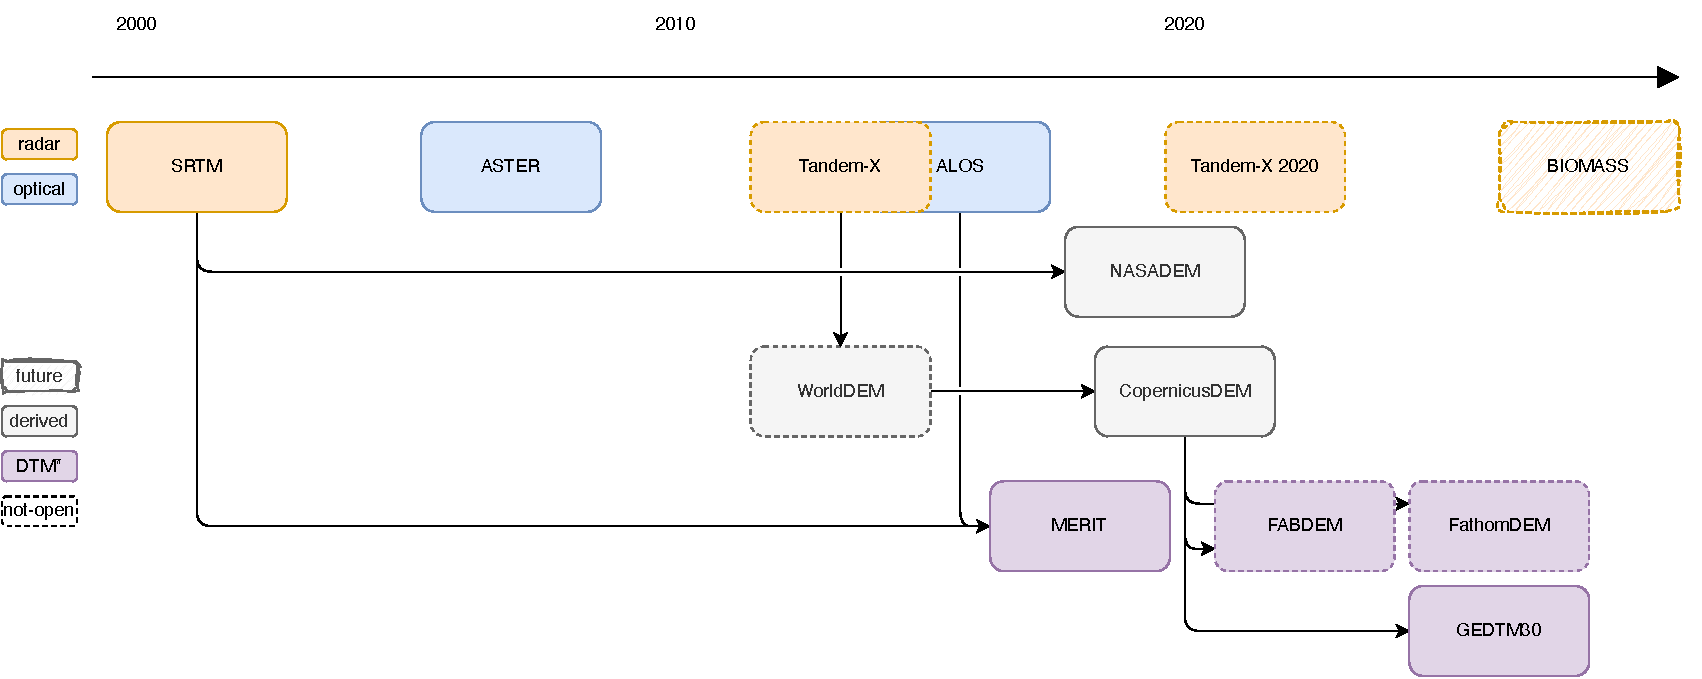
\includegraphics[width=\linewidth]{dems_overview}
  \caption{An overview of current gDEMs}%
  \label{fig:gdem_inheritance}
\end{figure*}
Note that all these products differ considerably in terms of coverage, resolution, accuracy and licensing.
Even the same product can have different versions, with different resolutions and licenses.

%

For example, SRTM is freely available,
\marginnote{SRTM}\index{SRTM}
including its derived NASADEM, and was first introduced at \qty{90}{m}, with subsequent versions at \qty{30}{m}.
Tandem-X, and its derived WorldDEM, is a commercial product, with a resolution of \qty{\pm12}{m}.
WorldDEM-NEO, a newer version of WorldDEM with more Tandem-X data (as used in Tandem-X 2020), even has a resolution of \qty{\pm5}{m}.
CopernicusDEM is a resampled WorldDEM---bought with your taxpayer money by ESA and freely distributed---at \qty{30}{m} resolution.
The pseudo DTMs FABDEM (\textbf{F}orest \textbf{A}nd \textbf{B}uilding removed) and FathomDEM, while derived from the freely available CopernicusDEM, are only free for research purposes.

Similarly, while ALOS World3D is freely available at \qty{30}{m}, it also comes in a commercial version at \qty{5}{m} resolution.
There is even a \qty{0.5}{m} commercial version, based on multiple optical satellites, available on request.

% We list only the ones available as open-access?
% For instance AW3D is also available as 5m-grid, but €€€.

% Maybe we should make our own table with paid products too? Like that table: \url{https://github.com/DahnJ/Awesome-DEM#summary}
% I find it interesting to know that some products are not free, and way better

% \usepackage{booktabs}
\begin{table*}[]
  \begin{tabular}{@{}lclllll@{}}
    \toprule
    & Year released & By                 & Sensor  & Type               & License & Resolution \\
    \midrule
    SRTM          & 2001          & NASA               & InSAR   & DSM                & Open    & 30--90m    \\
    ASTER         & 2009          & NASA               & optical & DSM                & Open    & 30m        \\
    Tandem-X      & 2014          & DLR                & InSAR   & DSM                & Closed  & 12m        \\
    WorldDEM      & 2014          & Airbus             & InSAR   & DSM/DTM$^{\prime}$ & Closed  & 5--12m     \\
    ALOS          & 2016          & JAXA               & optical & DSM                & Open    & 30m        \\
    MERIT         & 2017          & \citet{Yamazaki17} & InSAR   & DTM$^{\prime}$     & Open    & 90m        \\
    NASADEM       & 2019          & NASA               & InSAR   & DSM                & Open    & 30m        \\
    CopernicusDEM & 2020          & ESA                & InSAR   & DSM                & Open    & 30--90m    \\
    Tandem-X 2020        & 2022          & \citet{wessel2022}   & InSAR   & DSM     & Closed  & 30m        \\
    FABDEM        & 2022          & \citet{Hawker22}   & InSAR   & DTM$^{\prime}$     & Closed  & 30m        \\
    FathomDEM        & 2025          & \citet{uhe2025}   & InSAR   & DTM$^{\prime}$     & Closed  & 30m        \\
    GEDTM30        & 2025          & \citet{ho2025}   & InSAR   & DTM$^{\prime}$     & Open  & 30m        \\
    \bottomrule
  \end{tabular}
  \caption{Overview of global DEMS, see Figure~\ref{fig:dem_comparison} for their lineage.}%
  \label{tab:gdem_overview}
\end{table*}

% TODO: A few words about fusion? [Okolie22] has very long review.

\begin{figure*}
  \centering
  \begin{subfigure}[t]
    {0.45\linewidth}
    \includegraphics[width=\linewidth]{nasadem.png}
    \caption{NASADEM}\label{fig:nasadem}
  \end{subfigure}
  \qquad
  \begin{subfigure}[t]
    {0.45\linewidth}
    \includegraphics[width=\linewidth]{copernicusdem.png}
    \caption{CopernicusDEM}\label{fig:copernicusdem}
  \end{subfigure}
  \caption{NASADEM and CopernicusDEM for the Indus delta in Pakistan. Note the striped noise in NASADEM, and how CopernicusDEM has more detail. There is $\sim$twelve years between these images.}%
  \label{fig:dem_comparison}
\end{figure*}





%%%%%%%%%%%%%%%%%%%%
%
\section{Specific characteristics of gDEMs}[Specific characteristics]

%%
\subsection{Global often means near-global}

The data collected depend on the orbit of the satellite.
Some satellites have a polar orbit and can therefore completely measure the Earth (ICESat-2 is one example, see~\ref{fig:orbit}), while some will cover only certain latitudes (\eg\ GEDI, see~\ref{fig:orbit}).

Similarly, while the Tandem-X mission produced a DEM with a global coverage, the SRTM DEM was measured from the Space Shuttle and only covers up to \qty{60}{\degree} latitude.

%%
\subsection{Format}

The formats used to store and exchange DEMs have historically been defined by the military, which are still used by many government agencies.
One example is the \emph{Digital Terrain Elevation Data} (DTED) format, developed in the 1970s, which stores elevation in integers (which tells us a lot about the accuracy and precision possible 50 years ago).
It specifies several possible \emph{levels} in terms of resolution (in arcseconds), from level 0 at \qty{\pm1}{km} to level 2 at \qty{30}{m}.
More recently, in 2016, the Defence Gridded Elevation Data (DGED) has been defined, specifying more levels to higher resolutions and allowing GeoTIFFs to used (which removes the integer constraint).
\marginnote{GeoTIFF}
DGED also defines the structure and the specific tiling of the data at higher latitudes, as resolutions in arcseconds become smaller near the poles.

%
Most of the gDEMS are tiled in a similar way.
CopernicusDEM---adhering to the DGED level 3 standard---has tiles of 3601$\times$3601 pixels on the equator, but 3600$\times$2400 (height, width) pixels at \qty{50}{\degree} latitude, 3600$\times$1800 at \qty{60}{\degree} latitude, 3600$\times$1200 at \qty{70}{\degree} latitude, becoming as small as 3600$\times$360 for the last 5 degrees of latitude.
This tiling scheme results in pixels being as square as possible, but makes it hard to work with tiles from different latitudes.

In this context it becomes clear that the resolution should not be discussed in terms of meters, but terms of degrees (or divisions of a degree).
As the Earth has a circumference of \qty{\pm40000}{km} (measured around the Equator), \ang{1} of latitude is \qty{\pm111}{km} and \ang{1} of longitude is $111\cos\phi$ \unit{km} at latitude $\phi$.
Degrees are further divided into 60 arcminutes (\lq), which themselves are divided into 60 arcseconds (\lq\lq).
In practice, the highest resolution for SRTM (\qty{30}{m}) is actually \ang{;;1}, and its \qty{90}{m} product has a resolution of \ang{;;3}.
DTED level 0 thus has a resolution of \ang{;;30}, while level 2 has a resolution of \ang{;;1}.
%

Datasets such as SRTM and NASADEM can be provided as \texttt{.hgt} (height) files, which are not even a format, but are simply a binary file with the elevation values listed in a given order, with the geographic extent to be derived from the filename.
% GDAL can however read these files.


\begin{floatbox}
\begin{kaobox-practice}[frametitle=\faCog\ Downloading gDEMs]
Most of the gDEMS are available in a standard and easily accessible format, such as GeoTIFF\@.
However, for broad compatibility, recent advances such as new compression techniques and tiling strategies are not yet widely used.
\\ \\
One such advance is Cloud Optimized GeoTIFF (COG: \url{https://www.cogeo.org}), which is a normal GeoTIFF with a specific structure that allows it to be read piecewise from the cloud.
Without such a structure, a GeoTIFF has to be downloaded in its entirety---even if one is only interested in a small part of it---before it can be read.
\end{kaobox-practice}
\end{floatbox}

%%%
\subsection{Accuracy}

The accuracy of gDEMs is often broken down into several components and related metrics, which are not always well-defined.
The DTED and DGED specifications differentiate between horizontal and vertical accuracy, and within each defines both relative and absolute accuracy.
Relative accuracy describes the consistency of the measurements, specified as the random error component of the uncertainty between two DEM pixels. % this is related to precision
Absolute accuracy describes the total error of a measurement compared to a reference.

%

The DGED standard specifies a relative vertical accuracy of less than \qty{12}{m} for level 2 (resolution of \ang{;;1}, or \qty{\pm30}{m}) and an absolute accuracy (goal) of \qty{18}{m}.
CopernicusDEM reports a mean error of less than \qty{2}{m} for 65\% of its tiles, and another 19\% with an error of less than \qty{5}{m} in terms of absolute accuracy.


%%%
\subsection{Errors}

As with any measurements taken, gDEMs contain errors and outliers.
For example, SRTM contains a lot of noise, and has (diagonal) striping artefacts, visible in Figure~\ref{fig:nasadem} for the derived NASADEM\@.

%

Another example is CopernicusDEM that suffers from multipath errors in urban areas, which lead to small pits in the DEM, see Figure~\ref{fig:copernicus_error}.
\begin{figure*}
  \centering
  \includegraphics[width=\linewidth]{low_outliers.pdf}
  \caption{Low outliers in CopernicusDEM, with orthophoto on the right for context. Electricity poles, visible by their shadows, are the cause for these errors here.}%
  \label{fig:copernicus_error}
\end{figure*}

%

Most gDEMS suffer from voids in steep terrain, as peaks can occlude valleys below (called the shadow effect).
%%\paragraph{void filling: \url{https://en.wikipedia.org/wiki/Shuttle_Radar_Topography_Mission#Void-filled_SRTM_datasets}
\marginnote{voids in DEMs}
These voids are often filled not only by interpolation, but with the help of other gDEMS, as they measured the same area from a different angle.

%

Furthermore, gDEM products are often accompanied by a quality layer, which indicates where data has been void-filled.
Similarly, error masks with the calculated instrument error and water masks are often provided alongside the elevation data.



%%
% \paragraph{integration with sea-level datasets}
%%
% \paragraph{accuracy affected by slope (most image-based products)}


%%
\subsection{Vertical datums}

Global DEMs are vertically referenced to a specific geoid, specifically EGM96 (EPSG:5171) for SRTM and EGM2008 (EPSG:3855) for CopernicusDEM\@.%
\marginnote{Earth Gravitational Model (EGM)}
Be aware that there is a small difference---generally less than \qty{0.5}{m}---between these versions of the EGM geoid.

% MSS = Geoid + MDT
Note that the geoid is not the same as the mean sea level (MSL),%
\index{mean sea level (MSL)}\marginnote{mean sea level (MSL)}
as it does not take into account the dynamic effects of temperature and currents.
Depending on the location, the difference between the geoid and MSL can be up to \qty{1.5}{m}.


%%
\subsection{gDEMs are DSM (more than DTM)}

In contrast to local DEMs, which are often provided as either a classified point cloud, or as separate raster DSMs and DTMs, gDEMs should be classified as DSMs.
The current measurement techniques will measure the top of canopy and buildings, and not the ground below.
This is the largest source of error in gDEMS, and can considerably limit the applicability of the data.

%

Several attempts have been made to correct gDEMS for vegetation and buildings, leading to what we denote as a \emph{pseudo DTM} (DTM$^{\prime}$).
\marginnote{DTM$^{\prime} =$ pseudo DTM}
While these methods improve the accuracy of gDEMs considerably, they are not perfect, and resulting terrain still contain vegetation and/or buildings.
Recent work has also suggested that while these datasets have improved vertical accuracy, the accuracy of derived geomorphometric parameters such as slope and curvature suffers.
% are still far removed from a local DTM\@.

%%%%%%%%%%%%%%%%%%%%
%
\section{Notes and comments}

Space lidar is promising as a source to reconstruct gDEMs because lidar penetrates vegetation, and thus obtaining a DTM is an easier process.
Recently, several global \emph{coastal} pseudo DTMs---covering only areas near or below sea-level---have been produced using space lidar (to some extent): CoastalDEM~\citep{Kulp24}, DiluviumDEM~\citep{Dusseau23} and DeltaDTM~\citep{Pronk24}.
Likewise, the new ESA Biomass mission~\citep{quegan2019}---launched in 2025---will use P-band radar to penetrate vegetation and measure the ground below, potentially enabling a truly global DTM in the future.

\citet{Yang11} provide a detailed list of applications where gDEMs (SRTM, but when the paper was written (2011) SRTM was still the main product available globally) are necessary as input.

\citet{Schumann2018} make a case for the need for high-accuracy open-access DEMs, demonstrating SRTM is not good enough for many applications.

\citet{Hancock2021} investigates the requirements for a global lidar DEM\@.

Further reading about DEM terminology can be found in \citet{Guth2021}, which is one of the products of the \emph{Digital Elevation Model Intercomparison eXperiment} (DEMIX) group.
They also published a paper comparing the vertical accuracy and derived parameters of several gDEMs~\citep{guthRanking10Global2024}.

Arguably the best place to download DEMs (gDEMS, local ones, lidar datasets, etc.) is OpenTopography (\url{https://opentopography.org}).
Otherwise each gDEM has its own download portal, with its own registration systems and its specific ways of searching and downloading the data.
In case of the most recent gDEMS, such as CopernicusDEM, the data must be downloaded as \texttt{.tar} (archives) for \ang{1}$\times$\ang{1} tiles via FTP, in folders for each continent and then country.
Data is duplicated for the border areas, totalling \qty{2}{TB}.

To learn more about the DGED format, read \url{https://dgiwg.org/documents/dgiwg-standards}.
Similarly, reading a user guide on any of the gDEMS is a good idea, such as the one for \href{https://spacedata.copernicus.eu/documents/20126/0/GEO1988-CopernicusDEM-SPE-002_ProductHandbook_I3.0+%281%29.pdf}{CopernicusDEM Product Handbook}.

\citet{Hawker22} give the details how the vegetation and buildings are removed from CopernicusDEM to create FABDEM\@.

%%%%%%%%%%%%%%%%%%%%
%
\section{Exercises}

% TODO: think of some exam questions to put here
\begin{enumerate}
  \item How wide is 1 degree longitude at the latitude where the city of Delft is? And at the North Pole?
  \item How old is the oldest gDEM, and what latitudes did it cover?
  \item Assume you want to compare the elevations from AHN5 to those of CopernicusDEM\@. Which steps/conversions are needed?
\end{enumerate}
                   %- 03
%!TEX root = ../terrainbook.tex
% chktex-file 36
% chktex-file 46

% \setchapterpreamble[u]{\margintoc}
\setchapterpreamble[u]{\youtube[0pt]{youtu.be/ysLCuqcyJZA}\margintoc[18pt]}
\graphicspath{{dtvd/figs/}}


\newcommand{\Orient}{O\textsc{rientation}\xspace}
\newcommand{\walk}{W\textsc{alk}\xspace}
\newcommand{\Incircle}{I\textsc{n}C\textsc{ircle}\xspace}

\chapter{Delaunay triangulations \& Voronoi diagrams}%
\label{chap:dtvd}
% \marginnote{\faVideoCamera\ \url{https://youtu.be/ysLCuqcyJZA}}

Delaunay triangulations (DT) and Voronoi diagrams (VD) are fundamental data structures for terrains, both for their representation and for their processing (\eg\ interpolation and several operations on terrains and point clouds are based on one of these structures).

%

This chapter formally defines the VD and DT in two dimensions, and introduces several concepts in computational geometry and combinatorial topology that are needed to understand, construct, and manipulate them in practice. 
Delaunay triangulations with constraints are also discussed.


\section{Voronoi diagram}%
\label{sec:vd}%
\index{Voronoi diagram}

Let $S$ be a set of points in $\mathbb{R}^2$ (the two-dimensional Euclidean space). 
The Voronoi cell of a point $p \in S$, defined $\mathcal{V}_{p}$, is the set of points $x \in \mathbb{R}^2$ that are closer to $p$ than to any other point in $S$; that is:
\begin{equation}
\mathcal{V}_p = \{x \in \mathbb{R}^{2} \ | \ \|x-p\| \, \leq \, \|x-q\|, \ \forall \, q \in S \}. 
\end{equation}
The union of the Voronoi cells of all generating points $p \in S$ form the Voronoi diagram of $S$, defined VD($S$). 
If $S$ contains only two points $p$ and $q$, then VD($S$) is formed by a single line defined by all the points $x \in \mathbb{R}^2$ that are equidistant from $p$ and $q$. 
This line is the perpendicular bisector of the line segment from $p$ to $q$, and splits the plane into two half-planes. 
$\mathcal{V}_p$ is formed by the half-plane containing $p$, and $\mathcal{V}_q$ by the one containing $q$. 
\begin{marginfigure}
  \centering
  \includegraphics[width=\textwidth]{halfspaces}
  \caption{The Voronoi cell $\mathcal{V}_p$ is formed by the intersection of all the half-planes between $p$ and the other points. }% 
\label{fig:halfspaces}
\end{marginfigure}
As shown in Figure~\ref{fig:halfspaces}, when $S$ contains more than two points (let us say it contains $n$ points), the Voronoi cell of a given point $p \in S$ is obtained by the intersection of $n-1$ half-planes defined by $p$ and the other points $q \in S$. 
That means that $\mathcal{V}_{p}$ is always convex. 
Notice also that every point $x \in \mathbb{R}^2$ has at least one nearest point in $S$, which means that VD($S$) covers the entire space.

%

\begin{marginfigure}
  \centering
  \includegraphics[width=\textwidth]{vd_circle}
  \caption{The VD for a set $S$ of points in the plane (the black points). The Voronoi vertices (brown points) are located at the centre of the circle passing through three points in $S$, provided that this circle contains no other points in $S$ in its interior.}% 
\label{fig:vd_circle}
\end{marginfigure}
As shown in Figure~\ref{fig:vd_circle}, the VD of a set $S$ of points in $\mathbb{R}^2$ is a planar graph. 
Its edges are the perpendicular bisectors of the line segments of pairs of points in $S$, and its vertices are located at the centres of the circles passing through three points in $S$. 
The VD in $\mathbb{R}^2$ can also be seen as a two-dimensional cell complex where each 2-cell is a (convex) polygon (see Figure~\ref{fig:vd2d}). 
\begin{figure}
  \centering
  \includegraphics[page=3,width=\textwidth]{vd2d}
  \caption{VD of a set of points in the plane (clipped by a box). The point $p$ (whose Voronoi cell is dark grey) has seven neighbouring cells (light grey).}% 
\label{fig:vd2d}
\end{figure}
Two Voronoi cells, $\mathcal{V}_{p}$ and $\mathcal{V}_{q}$, lie on the opposite sides of the perpendicular bisector separating the points $p$ and $q$. 

%

The VD has many interesting properties, what follows is a list of the most relevant properties in the context of this course.
\begin{description}
  \item[Size:] if $S$ has $n$ points, then VD($S$) has exactly $n$ Voronoi cells since there is a one-to-one mapping between the points and the cells.
  \item[Voronoi vertices:] a Voronoi vertex is equidistant from 3 data points. Observe for instance in Figure~\ref{fig:vd_circle} that the Voronoi vertices are at the centre of circles.
  \item[Voronoi edges:] a Voronoi edge is equidistant from 2 points.
  \item[Convex hull:] let $S$ be a set of points in $\mathbb{R}^2$, and $p$ one of its points. $\mathcal{V}_{p}$ is unbounded if $p$ bounds conv($S$). Otherwise, $\mathcal{V}_{p}$ is the convex hull of its Voronoi vertices. Observe that in Figure~\ref{fig:vd_circle}, only the point in the middle has a bounded Voronoi cell.
\end{description}
  

%%%
%
\section{Delaunay triangulation}%
\label{sec:dt_definition}\index{Delaunay triangulation}

Let $\mathcal{D}$ be the VD of a set $S$ of points in $\mathbb{R}^2$. 
Since VD($S$) is a planar graph, it has a dual graph, and let $\mathcal{T}$ be this dual graph obtained by drawing straight edges between two points $p,q \in S$ if and only if $\mathcal{V}_{p}$ and $\mathcal{V}_{q}$ are adjacent in $\mathcal{D}$. 
Because the vertices in $\mathcal{D}$ are of degree 3 (3 edges connected to it), the graph $\mathcal{T}$ is a triangulation. 
$\mathcal{T}$ is actually called the Delaunay triangulation (DT) of $S$, and, as shown in Figure~\ref{fig:dt2da}, 
\begin{figure}
  \centering
   \includegraphics[page=4,width=\textwidth]{vd2d}
  \caption{The DT of a set of points in the plane (same point set as Figure~\ref{fig:vd2d}). The green circles show 2 examples of empty circumcircles.}%
\label{fig:dt2da}
\end{figure}
partitions the plane into triangles---where the vertices of the triangles are the points in $S$ generating each Voronoi cell---that satisfy the \emph{empty circumcircle} test (a circle is said to be \emph{empty} when no points are in its interior). 
If $S$ is in general position, then DT($S$) is unique.

%
\subsection{Convex hull}%
\label{sec:convexhull}\index{convex hull}

The DT of a set $S$ of points subdivides completely conv($S$), \ie\ the union of all the triangles in DT($S$) is conv($S$).

Let $S$ be a set of points in $\mathbb{R}^2$, the \emph{convex hull} of $S$, denoted conv($S$), is the minimal convex set containing $S$. 
It is best understood with the elastic band analogy: imagine each point in $\mathbb{R}^2$ being a nail sticking out of the plane, and a rubber band stretched to contain all the nails, as shown in Figure~\ref{fig:convex_hull}. 
When released, the rubber band will assume the shape of the convex hull of the nails. 
Notice that conv($S$) is not only formed by the edges connecting the points (the rubber band), but all the points of $\mathbb{R}^2$ that are contained within these edges (thus the whole polygon).
\begin{marginfigure}
  \centering
  \includegraphics[width=\textwidth]{convex_hull}
  \caption{The convex hull of a set of points in $\mathbb{R}^2$.}% 
\label{fig:convex_hull}
\end{marginfigure}

%
\subsection{Local optimality}
Let $\mathcal{T}$ be a triangulation of $S$ in $\mathbb{R}^2$. 
An edge $\sigma$ is said to be \emph{locally} Delaunay if it either:
\begin{description}
  \item[(i)] belongs to only one triangle, and thus bounds conv($S$), or
  \item[(ii)] belongs to two triangles $\tau_a$ and $\tau_b$, formed by the vertices of $\sigma$ and respectively the vertices $p$ and $q$, and $q$ is outside of the circumcircle of $\tau_a$ (see Figure~\ref{fig:local}). 
\end{description}
Figure~\ref{fig:local} gives an example that violates the second criteria: both $p$ and $q$ are contained by the circumcircles of their opposing triangles, \ie\ of $\tau_b$ and $\tau_a$ respectively.

\begin{marginfigure}
  \centering
  \includegraphics[width=\textwidth,page=1]{local}
  \includegraphics[width=\textwidth,page=2]{local}
  \caption{A quadrilateral that can be triangulated in two different ways. Only the top configuration is Delaunay. \textbf{(top)} $\sigma$ is locally Delaunay. \textbf{(bottom)} $\sigma$ is not locally Delaunay.}%
\label{fig:local}
\end{marginfigure}

In an arbitrary triangulation, not every edge that is locally Delaunay is necessarily an edge of DT($S$), but local optimality implies globally optimality in the case of the DT:
\begin{quote}
  Let $\mathcal{T}$ be a triangulation of a point set $S$ in $\mathbb{R}^2$. If every edge of $\mathcal{T}$ is locally Delaunay, then $\mathcal{T}$ is the Delaunay triangulation of $S$.
\end{quote}
This has serious implications as the DT---and its dual---are locally modifiable, \ie\ we can theoretically insert, delete or move a point in $S$ without recomputing DT($S$) from scratch.


%%%
%
\subsection{Angle optimality}
The DT in two dimensions has a very important property that is useful in applications such as finite element meshing or interpolation: the \emph{max-min angle optimality}. 
Among all the possible triangulations of a set $S$ of points in $\mathbb{R}^2$, DT($S$) maximises the minimum angle (max-min property), and also minimises the maximum circumradii. 
In other words, it creates triangles that are as equilateral as possible. 
Notice here that maximising the minimum angle is not the same as minimising the maximum, and the DT only guarantees the former.

%

In the context of modelling terrains, the max-min angle optimality ensures that a surface approximated with the set of lifted (Delaunay) triangles will be close to the original surface.
Figure~\ref{fig:notdelaunay} shows two examples of a hill, the left surface is a random triangulation of some sample points of the surface, and the right one is the Delaunay triangulation of the same set of points.
\begin{figure*}
  \centering
  \includegraphics[width=0.9\linewidth]{notdelaunay/notdelaunay}
  \caption{The same set of sample points of a hill is triangulated on the left with a random triangulation (non-Delaunay) and right with a Delaunay triangulation. The shape of the triangles is shown at the bottom by projecting them to the $xy$-plane.}%
\label{fig:notdelaunay}
\end{figure*}



%%%
\subsection{Lifting on the paraboloid}%
\label{sec:parabolic_lifting}

There exists a close relationship between DTs in $\mathbb{R}^{2}$ and convex polyhedra in $\mathbb{R}^{3}$. 

Let $S$ be a set of points in $\mathbb{R}^{2}$. 
The parabolic lifting map projects each vertex $v(v_{x}, v_{y})$ to a vertex $v^{+}(v_{x}, v_{y}, v_{x}^{2}+v_{y}^{2})$ on the paraboloid of revolution in $\mathbb{R}^{3}$. 
The set of points thus obtained is denoted $S^{+}$. 
Observe that the paraboloid in three dimensions defines a surface whose vertical cross sections are parabolas, and whose horizontal cross sections are circles. 

%

The relationship is the following: every triangle of the lower envelope of conv($S^{+}$) projects to a triangle of the Delaunay triangulation of $S$; this is illustrated in Figure~\ref{fig:paraboloid} for a simple DT\@. 
\begin{marginfigure}
  \centering
  \includegraphics[width=\textwidth]{paraboloid}
  \caption{The parabolic lifting map for a set $S$ of points $\mathbb{R}^2$.}%
\label{fig:paraboloid}
\end{marginfigure}

%

 Construction of the two-dimensional DT can be transformed into the construction of the convex hull of the lifted set of points in three dimensions (followed by a simple project to the two-dimensional plane).

\begin{floatbox}
  \begin{kaobox-practice}[frametitle=\faCog\ How does it work in practice?]
    Since it is easier to construct convex hulls (especially in higher dimensions, \ie\ 4+), the DT is often constructed with this approach, even in 2D. One popular and widely used implementation is Qhull (\url{http://www.qhull.org/}).
  \end{kaobox-practice}
\end{floatbox}


%%%
%
\subsection{Degeneracies}%
\label{sec:degeneracies}

The previous definitions of the VD and the DT assumed that the set $S$ of points is in general position, \ie\ the distribution of points does not create any ambiguity in the two structures. 
For the VD/DT in $\mathbb{R}^{2}$, the degeneracies, or special cases, occur when 3 points lie on the same line and/or when 4 points are cocircular. 
For example, in two dimensions, when four or more points in $S$ are cocircular there is an ambiguity in the definition of DT($S$). 
\begin{marginfigure}
  \centering
  \includegraphics[width=\textwidth]{degeneracies}
  \caption{The DT for four cocircular points in two dimensions is not unique (but the VD is).}%
\label{fig:degeneracies}
\end{marginfigure}
As shown in Figure~\ref{fig:degeneracies}, the quadrilateral can be triangulated with two different diagonals, and an arbitrary choice must be made since both respect the Delaunay criterion (points should not be on the interior of a circumcircle, but more than three can lie directly on the circumcircle).

This implies that in the presence of four or more cocircular points, DT($S$) is not unique. 
Notice that even in the presence of cocircular points, VD($S$) is still unique, but it has different properties. 
For example, in Figure~\ref{fig:degeneracies}, the Voronoi vertex in the middle has degree 4 (remember that when $S$ is in general position, every vertex in VD($S$) has degree 3). 
When three or more points are collinear, DT($S$) and VD($S$) are unique, but problems with the implementation of the structures can arise.


%%%
%
\section{Duality between the DT and the VD}[Duality DT/VD]%
\label{sec:duality}\index{duality}

Duality can have many different meanings in mathematics, but it always refers to the translation or mapping in a one-to-one fashion of concepts or structures. 
We use it in this course in the sense of the dual graph of a given graph. 
Let $G$ be a planar graph, as illustrated in Figure~\ref{fig:dual_graph} (black edges).
\begin{marginfigure}
  \centering
  \includegraphics[width=\textwidth]{dual_graph}
  \caption{A graph $G$ (black lines), and its dual graph $G^\star$ (dashed lines).}%
\label{fig:dual_graph}
\end{marginfigure}

Observe that $G$ can also be seen as a cell complex in $\mathbb{R}^{2}$. 
The duality mapping is as follows (also shown in details in Figure~\ref{fig:dualdetail}).
The dual graph $G^{\star}$ has a vertex for each face (polygon) in $G$, and the vertices in $G^{\star}$ are linked by an edge if and only if the two corresponding dual faces in $G$ are adjacent (in Figure~\ref{fig:dual_graph}, $G^{\star}$ is represented with dashed lines). 
Notice also that each polygon in $G^{\star}$ corresponds to a vertex in $G$, and that each edge of $G$ is actually dual to one edge (an arc in Figure~\ref{fig:dual_graph}) of $G^{\star}$ (for the sake of simplicity the dual edges to the edges on the boundary of $G$ are not drawn).

The VD and the DT are the best example of the duality between plane graphs.
As Figure~\ref{fig:dualdetail} demonstrates:
\begin{enumerate}
  \item a Voronoi cell is dual to a Delaunay vertex;
  \item a Voronoi edge is dual to a Delaunay edge;
  \item a Voronoi vertex is dual to a Delaunay triangle.
\end{enumerate}
Observe that, as shown in Figures~\ref{fig:vd2d} and~\ref{fig:dualdetail}, the location of a Voronoi vertex $v^{\star}$, which is dual to a Delaunay triangle $\tau$, is at the centre of the circumcircle of $\tau$; Appendix~\ref{app:equations} describes how to obtain the ($x,y$)-coordinates of the centre.
\begin{figure}
  \centering
  \begin{minipage}[c]{0.4\textwidth}
    \includegraphics[width=\textwidth]{dualdetail.pdf}
  \end{minipage}
  \begin{minipage}[c]{0.45\textwidth}
  % \hspace{1.1em}
    \centering
    \begin{tabular}{lcl}
    \toprule
    DT & & VD \\
    \midrule
    $\mathbf{\color{YellowGreen}{face}}$ & $\leftrightarrow$ & $\mathbf{\color{ForestGreen}{vertex}}$\\
    $\mathbf{\color{Blue}{vertex}}$ & $\leftrightarrow$ & $\mathbf{\color{SkyBlue}{face}}$\\
    $\mathbf{\color{Orange}{edge}}$ & $\leftrightarrow$ & $\mathbf{\color{Dandelion}{edge}}$\\
    \bottomrule
    \end{tabular}
  \end{minipage}
  \caption{Duality between the DT (dotted) and the VD (dashed).}%
\label{fig:dualdetail}
\end{figure}


%%%
%
\section{Incremental construction of the DT}[Incremental construction]%
\label{sec:dtconstruction}

Since the VD and the DT are dual structures, the knowledge of one implies the knowledge of the other one. 
In other words, if one has only one structure, she can always extract the other one. 
Because it is easier, from an algorithmic and data structure point of view, to manage triangles over arbitrary polygons (they have a constant number of vertices and neighbours), constructing and manipulating a VD by working only on its dual structure is simpler and usually preferred. 
When the VD is needed, it is extracted from the DT\@. 
This has the additional advantage of speeding up algorithms because when the VD is used directly intermediate Voronoi vertices---that will not necessarily exist in the final diagram---need to be computed and stored.

%

While there exists different strategies to construct at DT, we focus in this book on the \emph{incremental} method since it is easier to understand and implement.
An incremental algorithm is one where the structure is built incrementally; in our case this means that each point is inserted one at a time in a valid DT and the triangulation is updated, with respect to the Delaunay criterion (empty circumcircle), after each insertion. 
Observe that the insertion of a single point $p$ in a DT modifies only \emph{locally} the DT, \ie\ only the triangles whose circumcircle contains $p$ need to be deleted and replaced by new ones respecting the Delaunay criterion (see Figure~\ref{fig:insertion_deletion} for an example). 
\begin{marginfigure}
  \centering
  \includegraphics[width=0.9\textwidth]{insertion_deletion}
  \caption{\textbf{(top)} The DT before and \textbf{(bottom)} after a point $p$ has been inserted. Notice that the DT is updated only locally (only the yellow triangles are affected).}%
\label{fig:insertion_deletion}
\end{marginfigure}

%

In sharp contrast to this, other strategies to construct a DT (\eg\ divide-and-conquer and plane sweep algorithms, see Section~\ref{sec:notes}), build a DT in \emph{one} operation (this is a batch operation), and if another point needs to be inserted after this, the whole construction operation must be done again from scratch. 
That hinders their use for some applications where new data coming from a sensor would have to be added, or where we want to delete points because they are outliers.

%

The incremental insertion algorithm, and the other well-known algorithms, can all construct the DT of $n$ points randomly distributed in the Euclidean plane in $\mathcal{O}(n \log n)$.

%

Figure~\ref{fig:insertion_steps} illustrates the steps of the algorithm, and Algorithm~\ref{algo:insert1pt} its pseudo-code. 
\begin{figure*}
  \centering
  \includegraphics[width=0.9\linewidth]{insertion_steps}
  \caption{Step-by-step insertion, with flips, of a single point in a DT in two dimensions.}%
\label{fig:insertion_steps}
\end{figure*}
\begin{algorithm}[tb] 
  \DontPrintSemicolon\
  \KwIn{A DT($S$) $\mathcal{T}$, and a new point $p$ to insert}
  \KwOut{$\mathcal{T}^{p} = \mathcal{T} \cup \{p\}$ // the DT with point $p$}
  find triangle $\tau$ containing $p$\;
  insert $p$ in $\tau$ by splitting it in to 3 new triangles (flip13)\;
  push 3 new triangles on a stack\;
  \While{stack is non-empty}
  {
    $\tau = \{p,a,b\} \leftarrow$ pop from stack\;
    $\tau_{a} = \{a,b,c\} \leftarrow$ get adjacent triangle of $\tau$ having the edge $ab$\;
    \If{$c$ is inside circumcircle of $\tau$}
    {
      flip22 $\tau$ and $\tau_{a}$\;
      push 2 new triangles on stack\;
    }
  }
  \caption{Algorithm to insert one point in a DT}%
\label{algo:insert1pt}
\end{algorithm} 
In a nutshell, for the insertion of a new point $p$ in a DT($S$), the triangle $\tau$ containing $p$ is identified and then split into three new triangles by joining $p$ to every vertex of $\tau$. 
Second, each new triangle is tested---according to the Delaunay criterion---against its opposite neighbour (with respect to $p$); if it is not a Delaunay triangle then the edge shared by the two triangles is \emph{flipped} (a \emph{flip} is an operation to modify adjacent triangles, see below) and the two new triangles will also have to be tested later. 
This process stops when every triangle having $p$ as one of its vertices respects the Delaunay criterion.


%%%
\subsection{Initialisation: the big triangle or the infinite vertex}%
\label{sec:big_tr}

The DT of a set $S$ of points subdivides conv($S$), which means in practice that the triangles on the boundary of conv($S$) will not be adjacent to exactly 3 neighbouring triangles.

\begin{marginfigure}
  \centering
  \includegraphics[width=\textwidth]{big_tr}
  \caption[The big triangle containing all the dataset.]{The set $S$ of points is contained by a \emph{big triangle} formed by the vertices $o_1$, $o_2$ and $o_3$. Many triangles outside conv($S$) are created.}% 
\label{fig:big_tr}
\end{marginfigure}
\begin{marginfigure}
  \centering
  \includegraphics[width=0.6\textwidth]{infinite_vertex}
  \caption[The infinite vertex.]{The infinite vertex ($\infty$) is used to ensure that the triangles in DT($S$) are always adjacent to exactly 3 triangles. This DT contains 7 finite triangles and 5 infinite triangles.}% 
\label{fig:infinite_vertex}
\end{marginfigure}
Because it is convenient to store and manipulate triangles having exactly 3 neighbours, in practice most DT construction algorithms will use one of these two ``tricks'':
\begin{itemize}
  \item \textbf{Big triangle:} $S$ is entirely contained in a big triangle $\tau_{big}$ several times larger than the spatial extent of $S$; conv($S$) therefore becomes $\tau_{big}$. 
  Figure~\ref{fig:big_tr} illustrates this.
  The construction of DT($S$) is for example always initialised by first constructing $\tau_{big}$, and then the points in $S$ are inserted one by one. 
  \item \textbf{Infinite vertex:} a fictitious vertex is inserted at the ``infinity'', and therefore the edges on the boundary of conv($S$) are incident to ``infinite triangles'' formed by a convex hull edge and the infinite vertex, see Figure~\ref{fig:infinite_vertex}.
  This can be conceptually seen as embedding $S$ on a sphere, and adding the infinite vertex on the other side of the sphere.
  The infinite vertex is conceptually the same as the big triangle but is numerically more stable since the size of the big triangle does not need to be defined.
  Observe however that since the infinite vertex has no coordinates, the predicates \Orient\ and \Incircle\ used to construct a DT (see Section~\ref{sec:predicates}) cannot be used with the infinite vertex and infinite triangles, instead one should handle those with specific cases.
\end{itemize}

%

Using a big triangle or an infinite vertex has many practical advantages. 
First, since an edge is always guaranteed to be shared by two triangles, point location algorithms never ``fall off'' the convex hull. 
Second, when a single point $p$ needs to be inserted in DT($S$), this guarantees that $p$ is always inside an existing triangle; we thus do not have to deal explicitly with vertices added outside the convex hull. 
Third, identifying the vertices that bounds conv($S$) is easy: they have one incident triangle that has one or more of the big triangle vertices (or it contains the infinite vertex).
Fourth, the Voronoi cells of the points that bounds conv($S$) will be bounded, since the only unbounded cells will be the ones of the 3 points of $\tau_{big}$. 
This can help for some of the spatial analysis operations, for instance interpolation based on the VD (see Chapter~\ref{chap:interpol}).

%

The main disadvantage is that more triangles than needed are constructed. 
For example in Figure~\ref{fig:big_tr} only the shaded triangles would be part of DT($S$). 
The extra triangles can nevertheless be easily marked as they are the only ones containing at least one of the 3 points forming $\tau_{big}$. 

%

\begin{floatbox}
  \begin{kaobox-practice}[frametitle=\faCog\ How are DT created in practice?]
  Several implementations of the DT use a big triangle or the infinite vertex,  CGAL (\url{https://www.cgal.org/}) and startinpy (\url{https://github.com/hugoledoux/startinpy}) are two examples.
  Those will refer in their API to ``finite'' and ``infinite'' vertices, edges, and triangles.
  It is therefore essential to understand the mechanism to use those librairies, even if one is not constructing the DT herself.
  \end{kaobox-practice}
\end{floatbox}


%%%
\subsection{Point location with walking}% 
\label{sec:dtwalk}

To find the triangle containing the newly inserted point $p$, we can use the point-in-polygon test for every triangle (the standard GIS operation), but that brute-force operation would be very slow (complexity would be $\mathcal{O}(n)$ or a single point location since each triangle must be checked).

A better alternative is to use the adjacency relationships between the triangles, and use a series of \Orient\ tests, as described in Section~\ref{sec:predicates}, to navigate from one triangle to the other. 
The idea, called ``walking'', is shown in Figure~\ref{fig:walk} and details are given in the Algorithm~\ref{algo:walk}.
\begin{figure}
  \centering
  \includegraphics[width=0.7\textwidth]{walk}
  \caption{The Walk algorithm for a DT in two dimensions. The query point is $p$.}%
\label{fig:walk}
\end{figure}
\begin{algorithm}[t]
  \DontPrintSemicolon\
  \KwIn{A DT($S$) $\mathcal{T}$, a starting triangle $\tau$, and a query point $p$}
  \KwOut{$\tau_r$: the triangle in $\mathcal{T}$ containing $p$}
  \BlankLine\ 
  $\tau_r$ = None\;
  \While{$\tau_r$ == None}
  {
    visitededges = 0\;
    \For{$i \leftarrow 0$ \KwTo\ 2}
    {
      $\sigma_i \leftarrow$ get edge opposite to vertex $i$ in $\tau$\;
      \If{\Orient($\sigma_i, p$) $< 0$\nllabel{l:walk}} 
      {
        $\tau \leftarrow$ get neighbouring triangle of $\tau$ incident to $\sigma_i$\;
        break\;
      }
      visitededges += 1\;
    }  
    \If{$visitededges == 3$}
    {
      \tcp{all the edges of $\tau$ have been tested}
      $\tau_r$ = $\tau$\;
    }
  }
  Return($\tau_r$)
  \caption{W\textsc{alk}($\mathcal{T}$, $\tau$, $p$)}%
\label{algo:walk}
\end{algorithm}
The idea is as follows: in a DT($S$), starting from a triangle $\tau$ (it can be any), we move to one of the adjacent triangle of $\tau$ ($\tau$ has three neighbours, we choose one neighbour $\tau_i$ such that the query point $p$ and $\tau$ are on each side of the edge shared by $\tau$ and $\tau_i$) until there is no such neighbour, then the simplex containing $p$ is the current triangle $\tau$.
Notice that this algorithm is not affected by degenerate cases, and that if an \textrm{O}\textsc{rientation} test returns 0 (collinearity), then it is simply considered a positive result. 
This will ensure that if the query point $p$ is located exactly at the same position as one point in $S$, then one triangle incident to $p$ will be returned.

It should be mentioned that while it appears straightforward, the point location step is the biggest computational bottleneck for a DT implementation.
For a large dataset (\eg\ a lidar point cloud, see Chapter~\ref{chap:massive} for some massive examples), if several thousands/millions of triangles must be tested to find the one containing a give point, then it will be very slow; the insertion itself with a series of flips is generally since around 4 flips will be performed for a normal distribution of points.
In practice, because most real-world datasets will have a high \emph{spatial coherence} (in simple terms, two consecutive points in the dataset are close in reality; see Section~\ref{sec:spatial_coherence}), the time spent on walking will be minimised since most library will start the walk from the previously inserted point.


%%%
\subsection{Flips}
\begin{marginfigure}
  \centering
  \includegraphics[width=0.7\textwidth]{flip22}
  \caption{A \emph{flip22}.}%
\label{fig:flip22}
\end{marginfigure}
Flips are operations that modify \emph{locally} the triangulation.
There are 3 flip operations (the numbers refer to the number of triangles before and after the flip):
\begin{itemize}
  \item a \textbf{flip22} modifies the configuration of two adjacent triangles. 
  Consider the set $S = \{a, b, c, d\}$ of points in the plane forming a quadrilateral, as shown in Figure~\ref{fig:flip22}. 
  There exist exactly two ways to triangulate $S$: the first one contains the triangles $abc$ and $bcd$; and the second one contains the triangles $abd$ and $acd$. 
  Only the first triangulation of $S$ is Delaunay because $d$ is outside the circumcircle of $abc$. 
  A \emph{flip22} is the operation that transforms the first triangulation into the second, or vice-versa.
  It is performed in constant time $\mathcal{O}(1)$.
  \item a \textbf{flip13} is the operation of inserting a vertex inside a triangle, and splitting it into three triangles (see Figure~\ref{fig:flip13}).
  \item a \textbf{flip31} is the inverse operation that deletes a vertex (see Figure~\ref{fig:flip13}).
\end{itemize}
\begin{marginfigure}
  \centering
  \includegraphics[width=0.7\textwidth]{flip13}
  \caption{A \emph{flip13} and its inverse operation \emph{flip31}.}%
\label{fig:flip13}
\end{marginfigure}


%%%
\subsection{Controlling the flips}
To control which triangles have to be checked and potentially flipped, we use a stack\footnote{The first-in-last-out data structure: \url{https://en.wikipedia.org/wiki/Stack_(abstract_data_type)}}. 
When the stack is empty, then there are no more triangles to be tested, and we are guaranteed that all the triangles in the triangulation have an empty circumcircle.


%%%
\subsection{Predicates}%
\label{sec:predicates}\index{predicates}
Constructing a DT and manipulating it essentially require two basic geometric tests (called \emph{predicates}): \Orient\ determines if a point $p$ is left, right or lies on the line segment defined by two points $a$ and $b$; and \Incircle\ determines if a point $p$ is inside, outside or lies on a circle defined by three points $a$, $b$ and $c$. 
Both tests can be reduced to the computation of the determinant of a matrix:
\begin{equation}
  \textrm{O}\textsc{rientation}(a, b, p) = 
  \left| 
  \begin{array}{cccc}
    a_{x} & a_{y} & 1 \\
    b_{x} & b_{y} & 1 \\
    p_{x} & p_{y} & 1 
  \end{array} 
  \right| 
\end{equation}
\begin{equation}
  \textrm{I}\textsc{n}\textrm{C}\textsc{ircle}(a, b, c, p) = 
  \left| 
  \begin{array}{ccccc}
    a_{x} & a_{y} & a^{2}_{x} + a^{2}_{y} & 1 \\
    b_{x} & b_{y} & b^{2}_{x} + b^{2}_{y} & 1 \\
    c_{x} & c_{y} & c^{2}_{x} + c^{2}_{y} & 1 \\
    p_{x} & p_{y} & p^{2}_{x} + p^{2}_{y} & 1 
  \end{array} 
  \right|%
\label{eq:insphere}
\end{equation}


%%%%%%%%%%%%%%%%%%%%%%%%%%%%
\section{Data structures for storing a DT}[DT data structures]

A triangulation is simply a subdivision of the plane into polygons, and thus any data structure used in GIS can be used to store a triangulation.

\begin{description}
  \item[Simple Features:] while many use this (PostGIS and any triangulation you see in Shapefiles), this is not smart: (1) the topological relationships between the triangles are not stored; (2) the vertices are repeated for each triangle (and we know that for a Poisson distribution of points in the plane a given point has exactly 6 incident triangles).
  \item[Edge-based structures:] all the edge-based topological data structure used for storing planar graphs (\eg\ DCEL, half-edge, winged-edge, etc) can be used. These usually lead to large storage space.
\end{description}

Observe that in practice, if only the DT is wanted (and not the constrained one, see below), practitioners will often simply store the sample points and reconstruct on-the-fly the DT, since it is unique (if we omit points not in general position that is).

However, because it is simpler to manage triangles over arbitrary polygons (they always have exactly 3 vertices and 3 neighbours), data structures specific for triangulations have been developed and are usually used.

The simplest data structure, as shown in Figure~\ref{fig:tr_ds}, 
\begin{figure}
  \centering
  \includegraphics[width=\linewidth]{tr_ds}
  \caption{The triangle-based data structure to store efficiently a triangulation (and the adjacency relationships between the triangles).}%
\label{fig:tr_ds}
\end{figure}
considers the triangle as being its atom and stores each triangle with 3 pointers to its vertices and 3 pointers to its adjacent triangles. 
Observe that the order in which the vertices and adjacent triangles stored correspond to each other. 
This is an important property that allows an efficient retrieval of triangles in the Walk algorithm (Algorithm~\ref{algo:walk}) for instance.



%%%%%%%%%%%%%%%%%%%%%%%%%%%%
\section{Constrained and Conforming Delaunay Triangulations}[Constraints in DT]%
\index{Constrained DT}\index{CDT}\index{Conforming DT}

Given as input a set $S$ of points and straight-line segments in the plane, different triangulations of $S$ (so that the segments are respected) can be constructed. 
We are mostly interested in the \emph{constrained Delaunay triangulation} (ConsDT) and the \emph{conforming Delaunay triangulation} (ConfDT), see Figure~\ref{fig:cdt_example} for one example.
\begin{marginfigure}
  \centering
  \includegraphics[width=0.85\linewidth]{cdt_example}
  \caption{\textbf{(top)} A set $S$ of points and straight-line segments. \textbf{(middle)} Constrained DT of $S$. \textbf{(bottom)} Conforming DT of $S$; the Steiner points added are in red.}%
\label{fig:cdt_example}
\end{marginfigure}

%%%
%
\paragraph*{Constrained DT (ConsDT).}
Given a set $S$ of points and straight-line segments in $\mathbb{R}^2$, the ConsDT permits us to decompose the convex hull of $S$ into non-overlapping triangles, and every segment of $S$ appears as an edge in ConsDT($S$). 
ConsDT is similar to the Delaunay triangulation, but the triangles in ConsDT are not necessarily Delaunay (\ie\ their circumcircle might contain other points from $S$). 
The empty circumcircle for a ConsDT is less strict: a triangle is Delaunay if its circumcircle contains no other points in $S$ that are \emph{visible} from the triangle.
The constrained segments in $S$ act as visibility blockers. 
Figure~\ref{fig:cdt_buildings} shows one example.
\begin{figure*}
  \centering
  \includegraphics[width=0.95\textwidth]{cdtbuildings}
  \caption{The ConsDT of a set of segments. On the right, the triangle whose circumcircle is green is a Delaunay (no other points in its interior) and so is the triangle whose circumcircle is in purple (there is one point in its interior, but it cannot be seen because of the constrained segment).}%
\label{fig:cdt_buildings}
\end{figure*}

%

Without going into details about one potential algorithm, one way to construct a ConsDT($S$) is (see Figure~\ref{fig:cdt_steps}):
\begin{figure*}
  \centering
  \includegraphics[width=0.95\linewidth]{cdt_steps}
  \caption{Steps to construct a ConsDT.}%
\label{fig:cdt_steps}
\end{figure*}
\begin{enumerate}
  \item construct DT($S^p$), where $S^p$ is the set containing all the points in $S$ and the end points of the line segments (Figure~\ref{fig:cdt_steps}b)
  \item insert each line segment, each insertion will remove edges from DT($S^p$). In Figure~\ref{fig:cdt_steps}c 3 edges are removed.
  \item this creates 2 polygons that need to be retriangulated, in Figure~\ref{fig:cdt_steps}d there is a blue and a green one.
  \item retriangulate each separately, the Delaunay criterion needs to be verified only for the vertices incident to the triangles incident to the hole/polygon.
\end{enumerate}

%

Observe that the ConsDT can be used to triangulate polygons with holes (see Figure~\ref{fig:cdt_dog}), it suffices to remove the triangle outside the exterior boundary, but inside the convex hull.

\begin{figure*}[b]
  \centering
  \begin{subfigure}[b]{0.3\linewidth}
    \centering
    \includegraphics[page=1]{cdt_dog}
    \caption{}
  \end{subfigure}%
  \qquad %-- that adds some space between th 2 figures
  \begin{subfigure}[b]{0.3\linewidth}
    \centering
    \includegraphics[page=2]{cdt_dog}
    \caption{}
  \end{subfigure}%
  \qquad %-- that adds some space between th 2 figures
  \begin{subfigure}[b]{0.3\linewidth}
    \centering
    \includegraphics[page=3]{cdt_dog}
    \caption{}
  \end{subfigure}%
  \caption{\textbf{(a)} One polygon with 4 holes (interior rings). \textbf{(b)} its ConsDT\@. \textbf{(c)} its ConfDT (the Steiner point added is in red).}%
\label{fig:cdt_dog}
\end{figure*}


%%%
%
\paragraph*{Conforming DT (ConfDT).}
A ConfDT adds new points to the input $S$ (called \emph{Steiner} points) to ensure that the input segments are present in the triangulation.% 
\index{Steiner point}\marginnote{Steiner point}
As Figures~\ref{fig:cdt_example} and~\ref{fig:cdt_dog} show, the input straight-line segments will be potentially split into several collinear segments. 
The Steiner points have to be carefully chosen (where to put them is beyond the scope of this course).

Observe that each triangle in a ConfDT respects the Delaunay criterion, but that more triangles are present. 
If 2 segments are nearly parallel, many points could be necessary (for $m$ segments, up to $m^2$ could be necessary).


%%%
%
\section{Notes and comments}%
\label{sec:notes}

The DT and the VD have been discovered, rediscovered and studied many times and in many different fields, see \citet{Okabe00} for a complete history.
The VD can be traced back to 1644, when Descartes used Voronoi-like structures in Part III of his \emph{Principia Philosophi\ae}. 
The VD was used by \citet{Dirichlet50} to study quadratic forms---this is why the VD is sometimes referred to as \emph{Dirichlet tessellation}---but was formalised and defined by \citet{Voronoi08}. 
The first use of the VD in a geographical context is due to \citet{Thiessen11}, who used it in climatology to better estimate the precipitation average around observations sites; the DT was formalised by \citet{Delaunay34}. 

For the construction of the DT, the incremental algorithm was first described by \citet{Lawson72-1}.
\citet{Fortune87} describes a sweep-line one, and \citet{Guibas85} a divide-and-conquer algorithm.

The local optimality of a DT, which implies globally optimality in the case of the DT, was proven by \citet{Delaunay34} himself.
The \emph{max-min angle optimality} of the DT was firstly observed by \citet{Sibson78}.
This parabolic lifting was first observed by \citet{Brown79} (who used a spherical transformation), further described by \citet{Seidel82,Edelsbrunner86}. 

\citet{Liu05-1} explains the details of the infinite vertex.

The walking algorithm described in this chapter, with a few modifications, can perform point location in $\mathcal{O}(n^{1/3}$).
However, it is in theory not the fastest solution: \citet{Mucke99} and \citet{Devillers02} discuss alternatives that are optimal (\ie\ $\mathcal{O}(\log n)$).
However, they both note that optimal algorithms do not necessarily mean better results in practice because of the amount of preprocessing involved, the extra storage needed, and also because the optimal algorithms do not always consider the dynamic case, where points in the DT could be deleted. 

Several criteria for constructing data-dependent triangulations are discussed in \citet{Dyn90}. 
While these can be used, in practice it was proven that the Delaunay triangulation is still the triangulation that minimises the roughness of a surface~\citep{Wang01,Rippa90}

% TODO : complete this: uniqueness of the DT
% If the input points of the DT are not in general position, it is still possible to obtain a unique DT\@.
% This however means that 

\citet{Shewchuk97} shows that while the triangle-based data structure requires twice as much code as with the quad-edge (to store and construct a ConsDT), the result is that the code runs twice as fast and the memory requirement as about 2X less.
CGAL (\url{https://www.cgal.org/}), among many others, uses the triangle-based data structure.

Since a DT can be locally modified by adding one point (and not reconstructing the whole structure from scratch, see Figure~\ref{fig:insertion_deletion}), it is also possible to delete/remove one vertex from a DT with only local operations.
\citet{Mostafavi03} and \citet{Devillers09} describe algorithms.


%%%
%
\section{Exercises}

\begin{enumerate}
  \item A DT has 32 triangles and we insert a new point $p$ that falls inside one of the triangles. If we insert and update the triangulation (for Delaunay criterion), what is the number of triangles?
  \item Given the input formed of elevation points and breaklines below (both projected to the $xy$-plane), draw both the constrained and conforming Delaunay triangulation (an approximation is fine).  {\centering{\includegraphics[width=0.95\linewidth]{cdt_exercise}}}
  \item If a given vertex $v$ in a DT has 7 incident triangles, how many vertices will its dual polygon contain?
  \item Identify the 5 infinite triangles in Figure~\ref{fig:infinite_vertex}.
  \item A DT has 6 vertices, and 3 of these are forming the convex hull. How many triangles does the DT have?
  \item Assume you have 8 points located on a circle. Draw the DT and the VD of these 8 points.
  \item When inserting points in a DT (Algorithm~\ref{algo:insert1pt}), what happens if a new point is inserted directly on an edge? Line~2 states that the triangle is split into 3 new triangles, does it still hold?
\end{enumerate}
                   %- 04
\include{interpol/interpol}           %- 05
%!TEX root = ../terrainbook.tex

\graphicspath{{kriging/}}
% \setchapterpreamble[u]{\margintoc}
\setchapterpreamble[u]{\youtube[0pt]{youtu.be/ZaadzBvgE2s}\margintoc[18pt]}


\chapter{Spatial interpolation: kriging}%
\label{chap:kriging}

Kriging is a spatial interpolation method that was developed mostly by Georges Matheron based on the earlier work of Danie Krige, who created it to estimate the yield of gold mines in South Africa.
In contrast to other spatial interpolation methods, it involves creating a custom model that is fine-tuned using the statistical properties of each dataset.
In this way, kriging can take into account the specific characteristics of a dataset, often yielding better results than other interpolation methods.

Like other techniques based on geostatistical models, kriging relies on the fact that when one moves across space, values such as the gold content in rock or the elevation in a terrain have both a general spatial \emph{trend}\index{trend} (\eg\ a flat mean value, a fitted plane or a more complex polynomial defining a surface) and a certain spatially correlated \emph{randomness} (\ie\ closer points tend to have more similar values).
Both of these elements are modelled in kriging.

More than a single method, kriging comprises a family of related methods.
Within this chapter, we will look at two related types of kriging: simple kriging and ordinary kriging.
These treat the spatially correlated randomness in a similar way, but they make different assumptions about the trend in a dataset.

\section{Statistical background}

The physical processes that shape the world can be considered to be at least partly deterministic.
In the case of a terrain, the elevation is determined by processes that we can model (more or less accurately), such as plate tectonics, volcanic activity, and erosion.
However, these processes are too complex and not understood well enough to use them to obtain accurate elevation values.
Imagine, for instance, how difficult it would be to get an accurate elevation map of the world using only the shape of the tectonic plates and some other parameters (\eg\ their direction and speed of movement).

Because of this complexity, the value of complex properties, such as the elevation of a terrain, are usually treated in geostatistics as the result of what is known as a \emph{random}\marginnote{random process}\index{random process} or \emph{stochastic process}\marginnote{stochastic process}\index{stochastic process}.
In this context, randomness can be understood as the fact that the value of a property at an unsampled location is not known exactly, and so we cannot assign it an exact number.
Instead, we can make an educated guess of the value at that location by creating a statistical model of its possible values using a \emph{probability distribution}\marginnote{probability distribution}\index{probability distribution}, which we can associate with a function (\ie\ a \emph{probability distribution function}) or with a set of standard statistical measures, such as the mean and variance.

This situation is phrased in mathematical terms by saying that the value of the elevation property \(Z\) at a location \(x\) is a \emph{random variable}\marginnote{random variable}\index{random variable} \(Z(x)\).
For the sake of simplicity, we will usually omit the location and denote it just as \(Z\); or when working with multiple locations (\eg\ \(x_i\) and \(x_j\)), we will shorten their respective random variables (\(Z(x_i)\) and \(Z(x_j)\)) using subscripts (\(Z_i\) and \(Z_j\)).

In geostatistics, the most common way to express the general shape of the probability distribution of a random variable is in terms of its mean and its variance.
Here, the mean\marginnote{mean}\index{mean} (also called \emph{expectation}\marginnote{expectation}\index{expectation} or \emph{expected value}\marginnote{expected value}\index{expected value}) of a random variable \(Z\) is a sort of probability-weighted average of its possible values and is denoted as \(E[Z]\) or \(\mu\).
Meanwhile, the \emph{variance}\marginnote{variance}\index{variance} of a random variable \(Z\) is a measure of how far the values of \(Z\) will usually spread from its mean, and it is denoted as \(\mathrm{var}(Z)\) or \(\sigma^2\).
A small variance thus means that a few random samples of \(Z\) at nearby locations will likely form a tight cluster around its mean, whereas a large variance will have sample values that are more distant from the mean value.

Mathematically, the variance is defined as the expected value of the squared deviation from the expected value of \(Z\), or:

\begin{align}
\mathrm{var}(Z) &= E\left[{\left(Z-E\left[Z\right]\right)}^2\right] \label{eq:variance1} \\
&= E\left[Z^2 -2ZE\left[Z\right] + E[Z]^2\right] \nonumber \\
&= E\left[Z^2\right] - 2E\left[Z\right]E\left[Z\right] + E\left[Z\right]^2 \nonumber \\
&= E\left[Z^2\right] - 2E\left[Z\right]^2 + E\left[Z\right]^2 \nonumber \\
&= E\left[Z^2\right]-{E[Z]}^2. \label{eq:variance2}
\end{align}

Next, it is important to define the covariance\marginnote{covariance}\index{covariance}, denoted as \(\mathrm{cov}(Z_i,Z_j)\), or \(\sigma_{ij}\), which expresses the joint variability of the random variables \(Z_i\) and \(Z_j\).
Thus, a positive covariance between \(Z_i\) and \(Z_j\) means that when one increases/decreases, the other is expected to increase/decrease in the same direction.
Conversely, a negative covariance means that the variables tend to increase/decrease in opposite directions.
The magnitude of the covariance is related to the magnitude of this increase or decrease.
It is thus defined mathematically as the expected product of their deviations from their (individual) expected values, or:

\begin{align}
\mathrm{cov}(Z_i, Z_j) &= E\left[\left(Z_i-E[Z_i]\right) \left(Z_j-E[Z_j]\right)\right] \label{eq:covariance} \\
&= E\left[Z_iZ_j - Z_iE\left[Z_j\right] - E\left[Z_i\right]Z_j + E\left[Z_i\right]E\left[Z_j\right]\right] \nonumber \\
&= E\left[Z_iZ_j\right] - E\left[Z_i\right]E\left[Z_j\right] - E\left[Z_i\right]E\left[Z_j\right] + E\left[Z_i\right]E\left[Z_j\right] \nonumber \\
&= E\left[Z_iZ_j\right] - E\left[Z_i\right]E\left[Z_j\right]. \label{eq:covariance2}
\end{align}

Here, it is good to note that the covariance of \(Z_i\) with itself is equivalent to its variance:

\begin{equation}
\mathrm{cov}(Z,Z) = E\left[\left(Z-E[Z]\right)^2\right] = \mathrm{var}(Z). \nonumber
\end{equation}

While not used further in this lesson, it is also good to know that the variance and the covariance can be used to calculate the Pearson correlation coefficient\marginnote{correlation coefficient}\index{correlation coefficient} \(\rho_{ij}\), which is one of the most common statistical measures that is applied to datasets:

\begin{equation}
\rho_{ij}=\frac{\mathrm{cov}(Z_i, Z_j)}{\sqrt{\mathrm{var}(Z_i) \mathrm{var}(Z_j)}}. \nonumber
\end{equation}

Note that this is essentially just a normalised form of the covariance.

\section{Geostatistics and the standard geostatistical model}[Geostatistical model]

In geostatistics, we apply the concepts covered in the previous section on general-purpose statistics to consider how they work with spatial phenomena, where values have a location and are often \emph{spatially} correlated (not just correlated).

The model most commonly applied in geostatistics considers that a random variable \(Z\), which represents a spatially correlated property at a given location, can be decomposed into two related variables: (i) a non-random spatial trend that can be modelled by the expectation \(E[Z]\) (\eg\ using a constant, a polynomial, a spline, etc.); and (ii) a random but spatially correlated deviation from this trend that is considered as a sort of adjustment, error or residual term and is here denoted as \(R\).
In the case of elevation, the former would represent the general shape of the terrain, whereas the latter would represent local differences from it.
We therefore have:

\begin{equation}
\label{eq:geostat}
Z = E\left[Z\right] + R.
\end{equation}

The different types of kriging from this chapter model the trend in a different way but treat the residual term in a similar way.
These are:
\begin{itemize}
\item \emph{simple kriging}, where the trend is a known constant that we specify in the model; and
\item \emph{ordinary kriging}, where the trend is a local mean that we calculate in the interpolation process.
\end{itemize}

These will be described in detail later in the chapter.
However, in order to understand how these work and when they can be applied, it is important to cover some common properties of the two terms of the standard geostatistical model.

Regarding the expectation/trend, simple kriging relies on the assumption that the expectation \(E(Z)\) is the same everywhere, which is known as the \emph{stationarity of the mean}\marginnote{stationarity of the mean}\index{stationarity of the mean}.
In the case of a terrain, that could mean that a terrain is uneven with significant peaks and valleys, but that there is not a general trend across it (\eg\ a clear slope with higher elevations on one side and lower elevations on the opposite side).
Mathematically, we can express that as:

\begin{align}
\label{eq:stationarityofthemean}
E\left[Z(x+h\right)] = E\left[Z(x)\right],
\end{align}

where \(x\) is an arbitrary point in the domain (\ie\ the area we want to interpolate), \(h\) is any vector from \(x\) to another point in the domain and \(Z(x)\) is the value of a random variable at \(x\) (\eg\ its elevation).

Next, there are also important properties of the residual term.
First, note that since \(R = Z - E[Z] \), the variance (Equation~\ref{eq:variance1}) and covariance (Equation~\ref{eq:covariance}) can be defined in a simple way in terms of the residuals:

\begin{align}
\mathrm{var}\left(Z\right) &= E\left[{R}^2\right], \label{eq:varres} \\
\mathrm{cov}(Z_i,Z_j) &= E\left[R_i \cdot R_j\right]. \label{eq:covres}
\end{align}

Then, since we know that the expectation is by definition the mean, in order not to introduce any bias, the expected value of the residual must be zero, \ie\ \(E\left[R\right] = 0\).
When this is fulfilled, the model is said to be \emph{unbiased}\marginnote{unbiased}\index{unbiased}.
The way that is is achieved varies in different types of kriging.

Finally, another common assumption is that the residual term at a pair of locations does not depend on the locations, but instead can be defined based only on the vector separating them.
In the case of a terrain, this would mean that the likelihood of finding similar elevations at two points separated by a given distance and orientation does not change across the terrain.
For instance, a terrain that goes from smooth on one side to rough on the other would not satisfy this assumption.
Mathematically, we can express this using the covariance as:

\begin{align}
\label{eq:stationarityofthecovariance}
\mathrm{cov}\left(Z(x+h), Z(x)\right) = C(h),
\end{align}

where \(C\) is the covariance function.
Since both the expectation (Equation~\ref{eq:stationarityofthemean}) and the covariance (Equation~\ref{eq:stationarityofthecovariance}) are translation invariant, this pair of assumptions are together known as \emph{second-order stationarity}\marginnote{second-order stationarity}\index{second-order stationarity}.

\section{Covariance, dissimilarity and the semivariogram}%
\index{variogram}

According to the standard geostatistical model described above, the residual term is spatially correlated.
That is, even after removing the general spatial trend from a dataset, nearby samples will tend to have more similar values than those farther apart.
In kriging, we exploit that property by modelling it through a \emph{semivariogram} or a \emph{covariance function}.
These are roughly opposites, since the semivariogram is a measure of dissimilarity and the covariance is a measure of similarity.
However, both attempt to measure how much spatial correlation there is as a function of distance and both can be used with kriging.

The semivariogram \(\gamma(h)\)\marginnote{semivariogram}\index{semivariogram}, often just called a variogram\marginnote{variogram}\index{variogram} for short, is a function that expresses the average dissimilarity of the value of a random variable \(Z\) between sample points at different distances.
It is defined as:

\begin{equation}
\label{eq:semivariogram}
\gamma(h) = \frac{1}{2} (Z(x+h) - Z(x))^2,
\end{equation}

where \(x\) is a sample point, \(h\) is a vector from \(x\) to another sample point and \(Z(x)\) is the value of a random variable at \(x\) (\eg\ its elevation).
Note that the `semi' in semivariogram comes from the \(1/2\) in Equation~\ref{eq:semivariogram}.

When this is done with every possible pair of sample points in a dataset, or with a representative subset in order to speed up the process as it is usually done in practice, \(|h|\) (\ie\ the magnitude of the vector \(h\)) and \(\gamma(h)\) can be put into a scatter plot to show how the average dissimilarity of a value changes with the distance between the sample points.
The result of such a plot is what is known as a \emph{variogram cloud}\marginnote{variogram cloud}\index{variogram cloud} (Figure~\ref{fig:variogram_cloud}).

\begin{figure*}[htbp]
\begin{subfigure}{0.5\linewidth}
\centering
\includegraphics[width=\linewidth]{figs/data}
\caption{dataset}
\end{subfigure}%
\begin{subfigure}{0.5\linewidth}
\centering
\includegraphics[width=\linewidth]{figs/variogram_cloud}
\caption{variogram cloud}
\end{subfigure}%
\caption{Starting from (a) a sample dataset, (b) the variogram cloud can be computed.
In this case, only 1\% randomly selected point pairs were used.}%
\label{fig:variogram_cloud}
\end{figure*}

In this figure, it is possible to see some typical characteristics of a variogram cloud.
Since nearby sample points tend to have similar values, the dissimilarity tends to increase as the distance between sample points increases.
However, it is worth noting that since the farthest away pairs of sample points have similar values in this specific dataset, the dissimilarity also decreases at the highest distances.

Since most of the time there is a wide variation between the dissimilarities shown at all distances in a variogram cloud, the next step is to average the dissimilarity of the pairs of sample points based on distance intervals.
Mathematically, a series of averages of dissimilarities \(\gamma^\star(h)\), known as \emph{experimental semivariances}\marginnote{experimental semivariance}\index{experimental semivariance}, can be created by computing the average dissimilarities for all vectors whose lengths are within a series of specified intervals (generally known as \emph{bins} or \emph{lags}).
\marginnote{intervals (bins)}
Given a set \(\mathfrak{h}\) containing the vectors for a distance interval, the experimental semivariances are computed as:

\begin{equation}
\gamma^\star(\mathfrak{h}) = \frac{1}{2n}\sum\left(z\left(x+h\right)-z\left(x\right)\right)^2 \hspace{1cm}\text{for all } h \in \mathfrak{h}
\end{equation}

where \(n\) is the number of sample point pairs in \(\mathfrak{h}\).

This computation results in much smoother values for the dissimilarity, and the values of \(\gamma^\star(h)\) for all values of \(|h|\) are known as an \emph{experimental}\marginnote{experimental variogram}\index{experimental variogram} or \emph{empirical variogram}\marginnote{empirical variogram}\index{empirical variogram} (Figure~\ref{fig:experimental_variogram}a).
Figure~\ref{fig:experimental_variogram}b shows the relationship between the experimental semivariances, covariances and variance.
\begin{figure*}[htbp]
\begin{subfigure}{0.5\linewidth}
\centering
\includegraphics[width=\linewidth]{figs/experimental_variogram}
\caption{experimental variogram}
\end{subfigure}%
\begin{subfigure}{0.5\linewidth}
\centering
\includegraphics[width=\linewidth]{figs/semivariance_covariance}
\caption{parameters}
\end{subfigure}%
\caption{(a) The experimental variogram and (b) the relationship between the experimental semivariances, covariances and variance.}%
\label{fig:experimental_variogram}
\end{figure*}

Note that in order to avoid the unreliable dissimilarities that are common at large distances between sample points, it is usual practice to only compute the experimental variogram for distances up to about half of the size of the region covered by the dataset.

From the scatterplot of the experimental variogram, it is possible to see how a few important parameters can be used to describe it (Figure~\ref{fig:example_variogram}): 
\begin{itemize}
  \item the \emph{sill}\marginnote{sill}\index{sill}, which is the upper bound of \(\gamma^\star(h)\);
  \item the \emph{range}\marginnote{range}\index{range}, which is the value of \(|h|\) when it converges; 
  \item the \emph{nugget}\marginnote{nugget}\index{nugget}, which is the value of \(\gamma^\star(h)\) when \(|h|\) approaches 0.
\end{itemize}
\begin{figure}[htbp]
\centering
\includegraphics[width=\linewidth]{figs/example_variogram}
\caption{An experimental variogram can be described in terms of a few parameters.}%
\label{fig:example_variogram}
\end{figure}

Finally, the last step is to use these parameters to replace the experimental variogram with a \emph{theoretical variogram function}\marginnote{theoretical variogram function}\index{theoretical variogram function} that approximates it and which can be more easily evaluated for further calculations.
Depending on the shape of the variogram, there are various functions that can be used.
Some examples are:

\begin{align}
\gamma_\mathrm{circular}(h) &= \begin{cases}
  s \left(1-\frac{2}{\pi}\cos^{-1}\left(\frac{|h|}{r}\right)+\frac{2|h|}{\pi r}\sqrt{1-\frac{|h|^2}{r^2}}\right) + n & \text{if } |h| \leq r \\
  s + n & \text{if } |h| > r
  \end{cases}\\
\gamma_\mathrm{cubic}(h) &= \begin{cases}
  s \left(\frac{7|h|^2}{r^2}-\frac{8.75|h|^3}{r^3}+\frac{3.5|h|^5}{r^5}-\frac{0.75|h|^7}{r^7}\right) + n & \text{if } |h| \leq r \\
  s + n & \text{if } |h| > r
  \end{cases}\\
\gamma_\mathrm{exponential}(h) &= s \left(1 - e^\frac{-3|h|}{r}\right) + n \\
\gamma_\mathrm{gaussian}(h) &= s \left(1 - e^\frac{-\left(3|h|\right)^2}{r^2}\right) + n \\
\gamma_\mathrm{linear}(h) &= \begin{cases}
  \frac{s|h|}{r} + n & \text{if } |h| \leq r \\
  s + n & \text{if } |h| > r
  \end{cases}\\
\gamma_\mathrm{power}(h) &= \begin{cases}
  \frac{sr^2}{|h|^2} + n & \text{if } |h| \leq r \\
  s + n & \text{if } |h| > r
  \end{cases}\\
\gamma_\mathrm{spherical}(h) &= \begin{cases} 
   s \left(\frac{3|h|}{2r} - \frac{|h|^3}{2r^3}\right) + n & \text{if } |h| \leq r \\
   s + n & \text{if } |h| > r
  \end{cases}
\end{align}

where \(s\) is the \emph{sill}, set to roughly the value of \(\gamma^\star(h)\) when \(\gamma^\star(h)\) is  flat; \(r\) is the \emph{range}, roughly the minimum value of \(|h|\) where \(\gamma^\star(h)\) is flat, and \(n\) is the nugget, which is the starting value of \(\gamma^\star(h)\).
Figure~\ref{fig:theoretical_variogram} shows the result of fitting the example theoretical variogram functions.
Note how the cubic and especially the Gaussian functions are a good fit in this case.

\begin{figure*}[htbp]
\begin{subfigure}{0.33\linewidth}
\centering
\includegraphics[width=\linewidth]{figs/model_circular}
\caption{Circular}
\end{subfigure}%
\begin{subfigure}{0.33\linewidth}
\centering
\includegraphics[width=\linewidth]{figs/model_cubic}
\caption{Cubic}
\end{subfigure}%
\begin{subfigure}{0.33\linewidth}
\centering
\includegraphics[width=\linewidth]{figs/model_exponential}
\caption{Exponential}
\end{subfigure}\\
\begin{subfigure}{0.33\linewidth}
\centering
\includegraphics[width=\linewidth]{figs/model_gaussian}
\caption{Gaussian}
\end{subfigure}%
\begin{subfigure}{0.33\linewidth}
\centering
\includegraphics[width=\linewidth]{figs/model_linear}
\caption{Linear (bounded)}
\end{subfigure}%
\begin{subfigure}{0.33\linewidth}
\centering
\includegraphics[width=\linewidth]{figs/model_power}
\caption{Power (bounded)}
\end{subfigure}\\
\begin{subfigure}{0.33\linewidth}
\centering
\includegraphics[width=\linewidth]{figs/model_spherical}
\caption{Spherical}
\end{subfigure}%
\caption{Some possible theoretical variogram functions}%
\label{fig:theoretical_variogram}
\end{figure*}

Many other theoretical variogram functions are possible, \eg\ circular, cubic, linear, etc.
However, the three described above are the most common found in practice.

Before moving on to apply these to kriging, there are a couple of important points.
First, note that these theoretical functions are often only applied when \(|h| > 0\), since setting \(\gamma(0) = 0\) helps to ensure that kriging passes exactly through the sample points (the exact property as explained in Section~\ref{sec:interpol_properties}).
Second, all of the semivariogram-related functions seen in this section can be converted to covariance functions as well, taking into account that \(\gamma(h) = \mathrm{sill} - C(h)\).
Note that this means that the covariance is high when \(|h|\) is small and it decreases as \(|h|\) increases.

\section{Simple kriging}

Simple kriging is similar to other spatial interpolation methods that use a weighted average.
It starts from the assumption of second-order stationarity.
Moreover, the expectation is also known, and so the general procedure to perform it is to: (i) subtract it from the sample points to obtain residuals, (ii) use the residuals to define a function that estimates the value of the residual term at any location, and (iii) interpolate at the desired locations using the function added to the expectation.

Thus, simple kriging defines a function \(\hat{R}_0\) that estimates the value of the residual \(R\) of the random variable \(Z\) at a location \(x_0\) as a weighted average of its residuals at the \(n\) sample points \(x_i\) that we will use for the interpolation (where \(1 \leq i \leq n\)).
We denote this as:

\begin{equation}
\label{eq:wask}
\hat{R}_0 = \hat{Z}_0 - E[Z_0] = \sum_{i=1}^n w_i (\underbrace{Z_i-E[Z_i]}_{R_i}).
\end{equation}

Simple kriging is unbiased, and therefore the expected value of the estimation at a location \(x_0\) is equal to the expected value at that location.
In mathematical terms, we can formulate this as:

\begin{equation}
\label{eq:unbiased}
E\left[ \hat{Z}_0 - Z_0 \right] = 0 \hspace{1cm}\text{or}\hspace{1cm}E\left[Z_0\right] = E\left[ \hat{Z}_0 \right].
\end{equation}

% In order to check this for simple kriging, we can put the weighted average from Equation~\ref{eq:wask} in this equation, which results in the following:

% % TODO : why is latex complaining at \end{align} I removed \cancelto{} and it's solved
% \begin{align}
%   E\left[ Z_0 \right] &= E\left[ E[Z_0] + \sum_{i=1}^n w_i R_i \right] \nonumber \\
%   &= E[Z_0] + \sum_{i=1}^n w_i 0{E[R_i]} \nonumber \\
%   &= E[Z_0].  \nonumber
% \end{align}

Then, in order to derive the equations used in simple kriging, we start from the fact that it \emph{minimises the variance of the estimation error}\marginnote{minimisation of the variance}\index{minimisation of the variance}, which in this case is given by \(\mathrm{var}\left(\hat{R}_0 - R_0\right)\).
If we use the definition of the variance from Equation~\ref{eq:variance1}, this can be instead put in terms of an expectation:

\begin{equation}
\mathrm{var}\left(\hat{R}_0 - R_0\right) = E \left[ \left( \left(\hat{R}_0 - R_0\right) - E \left[\hat{R}_0 - R_0\right] \right)^2 \right] \nonumber
\end{equation}

However, we know from the unbiased criterion from Equation~\ref{eq:unbiased} that \(E\left[ \hat{R}_0 - R_0 \right] = 0\), and so we can simplify the previous equation as:

\begin{equation}
\mathrm{var}\left(\hat{R}_0 - R_0\right) = E\left[\left( \hat{R}_0 - R_0 \right)^2\right] \nonumber.
\end{equation}

If this is expanded, it results in:

\begin{align}
\mathrm{var}\left(\hat{R}_0 - R_0\right) &= E\left[{\hat{R}_0}^{\hspace{1.2mm}2} - 2\hat{R}_0R_0 + {R_0}^2 \right] \nonumber \\
&= E\left[{\hat{R}_0}^{\hspace{1.2mm}2}\right] - 2E\left[\hat{R}_0R_0\right] + E\left[{R_0}^2 \right] \nonumber \\
&= E\left[\sum_{i=1}^n \sum_{j=1}^n w_i w_j R_i R_j\right] - 2E\left[\sum_{i=1}^n w_i R_i R_0\right] + E\left[{R_0}^2 \right] \nonumber \\
&= \sum_{i=1}^n \sum_{j=1}^n w_i w_j E\left[R_i R_j\right] - 2\sum_{i=1}^n w_i E\left[R_i R_0\right] + E\left[{R_0}^2 \right]. \nonumber
\end{align}

Here, we can use the definitions of the variance based on residuals from Equations~\ref{eq:varres} and~\ref{eq:covres} together with our covariance formula from Equation~\ref{eq:stationarityofthecovariance}, which yields:

\begin{align}
\mathrm{var}\left(\hat{R}_0 - R_0\right) &= \sum_{i=1}^n \sum_{j=1}^n w_i w_j \mathrm{cov}(R_i, R_j) - 2\sum_{i=1}^n w_i \mathrm{cov}(R_i,R_0) + \mathrm{cov}(R_0, R_0) \label{eq:variancesk} \\
&= \sum_{i=1}^n \sum_{j=1}^n w_i w_j C(x_i-x_j) - 2\sum_{i=1}^n w_i C(x_i-x_0) + C(x_0-x_0).
\end{align}

In order to minimise this equation, we can find where its first derivative is zero.
This is:

\begin{equation}
\frac{\partial \mathrm{var}\left(\hat{R}_0 - R_0\right)}{\partial w_i} = 2 \sum_{j=1}^n w_j C(x_i-x_j) - 2C(x_i-x_0) = 0 \hspace{1cm} \text{for all } 1 \leq i \leq n, \nonumber
\end{equation}

which yields the set of \(n\) simple kriging equations:

\begin{equation}
\sum_{j=1}^n w_j C(x_i-x_j) = C(x_i-x_0).
\end{equation}

While these equations can be used to perform simple kriging, it is often easier to deal with these in matrix form:

\begin{equation}
\underbrace{\left(\begin{array}{c}
w_1 \\
\vdots \\
w_n \end{array} \right)}_{w}
%
\underbrace{\left( \begin{array}{ccc}
C(x_1-x_1) & \cdots & C(x_1-x_n) \\
\vdots & \ddots & \vdots \\
C(x_n-x_1) & \cdots & C(x_n-x_n) \end{array} \right)}_{A}
 = 
%
\underbrace{\left(\begin{array}{c}
C(x_1-x_0) \\
\vdots \\
C(x_n-x_0) \end{array} \right)}_{d}
\end{equation}

which is known as the \emph{simple kriging system}\marginnote{simple kriging system}\index{simple kriging system}.
Finally, if we invert the matrix \(A\), the weights are given by:

\begin{equation}
w = A^{-1}d.
\end{equation}

These weights can be applied to interpolate the value of the residual term at any location as a weighted average of the sample points, where the correlation between the points is given by a covariance function, which can be obtained from the semivariogram.

However, simple kriging does not tell us what value we should use for the expectation \(E[Z]\), since we start from the assumption that it is known, which is often not the case.
Even a seemingly reasonable value, such as average of all points, can be very inaccurate if the sample points are unevenly distributed across the domain.

\section{Ordinary kriging}%
\index{ordinary kriging}

Ordinary kriging is similar to simple kriging in that it estimates values using a weighted average function with weights computed from the semivariogram/covariance based on the distance between the points. 
However, it estimates a value at a location using only sample points in the neighbourhood of the location and relies only on \emph{local} second-order stationarity, \ie\ a constant mean within a moving neighbourhood, with a mean that is computed within the method itself.

Rather than relying on the residuals, it defines a function \(\hat{Z}_0\) that directly estimates the value of the random variable \(Z\) at a location \(x_0\) as a weighted average of its value at the \(n\) neighbouring sample points \(x_i\) that we will use for the interpolation (where \(1 \leq i \leq n\)).
We denote this as:

\begin{equation}
\label{eq:waok}
\hat{Z}_0 = \sum_{i=1}^n w_i Z_i.
\end{equation}

Like simple kriging, ordinary kriging is \emph{unbiased}, which is achieved by making sure that the interpolation weights add up to one, \ie\ \(\sum_{i=1}^n w_i = 1\).
Ordinary kriging also \emph{minimises the variance of the estimation error}, which is given by \(\mathrm{var}\left(\hat{Z}_0 - Z_0\right)\).
For this, we can use the same derivation as for simple kriging up to Equation~\ref{eq:variancesk} but using the variogram for the final step.
This is:

\begin{align}
\mathrm{var}\left(\hat{R}_0 - R_0\right) &= \sum_{i=1}^n \sum_{j=1}^n w_i w_j \mathrm{cov}(R_i, R_j) - 2\sum_{i=1}^n w_i \mathrm{cov}(R_i,R_0) + \mathrm{cov}(R_0, R_0) \nonumber \\
&= -\sum_{i=1}^n \sum_{j=1}^n w_i w_j \gamma(x_i-x_j) + 2\sum_{i=1}^n w_i \gamma(x_i-x_0) - \gamma(x_0-x_0).
\end{align}

Using the previous equation and the unbiased criterion from Equation~\ref{eq:unbiased}, we can apply the minimisation method known as Lagrange multipliers\footnote{\url{https://en.wikipedia.org/wiki/Lagrange_multiplier}} and arrive at the set of \(n+1\) ordinary kriging equations:

\begin{align}
\sum_{j=1}^n w_i \gamma(x_i-x_j) + \mu(x_0) &= \gamma(x_i - x_0) \hspace{1cm} \text{for all } 1 \leq i \leq n \nonumber \\
\sum_{j=1}^n w_i &= 1 
\end{align}

where \(\mu(x_0)\) is a Lagrange parameter that was used in the minimisation process.

Like with simple kriging, these equations can be used to perform ordinary kriging, but it is often easier to deal with these in matrix form:

\begin{equation}
%
\underbrace{\left( \begin{array}{cccc}
\gamma(x_1-x_1) & \cdots & \gamma(x_1-x_n) & 1 \\
\vdots & \ddots & \vdots & 1 \\
\gamma(x_n-x_1) & \cdots & \gamma(x_n-x_n) & 1 \\
1 & \cdots & 1 & 0 \end{array} \right)}_{A}
%
\underbrace{\left(\begin{array}{c}
w_1 \\
\vdots \\
w_n \\
\mu(x_0) \end{array} \right)}_{w} = 
%
\underbrace{\left(\begin{array}{c}
\gamma(x_1-x_0) \\
\vdots \\
\gamma(x_n-x_0) \\
1 \end{array} \right)}_{d}
\end{equation}

which is known as the \emph{ordinary kriging system}\marginnote{ordinary kriging system}\index{ordinary kriging system}.

Finally, if we invert the matrix \(A\), the weights and the Lagrange multipliers are given by:

\begin{equation}
w = A^{-1}d
\end{equation}

%%%
%
\section{Other types of kriging}

\begin{description}
\item[Directional kriging] is useful when the similarity of points differs according to different directions, \eg\ north-south versus east-west.
It involves creating variograms for different directions.
\item[Block kriging] attempts to obtain a local trend for an area around a point (rather than just at a point).
It can be used to obtain smoother results.
\item[Cokriging] applies kriging to multiple correlated variables.
It is particularly useful when you want to interpolate one variable with limited sample points but there are more sample points for another correlated variable.
\item[Indicator kriging] applies thresholds to obtain discrete values, such as presence/absence of a variable or a set of distinct classification classes.
\item[Poisson kriging] applies kriging to data involving cumulative counts or rates.
It is often applied together with polygonal datasets.
\item[Universal kriging] fits the trend using a predefined deterministic function.
It is tricky to use in practice because it imposes conditions on the underlying variogram.
\end{description}

%%%
%
\section{Implementation details}

There are a few important details with respect to the implementation of kriging methods in practice.

First of all, within this chapter, we have assumed that you always use all sample points to interpolate any point on the plane.
While this is optimal in theory, if a large number of sample points are used to interpolate every point, kriging can be \emph{very slow} in practice.
The reason for this is because matrix \(A\) will be very large, and inverting a matrix is a computationally expensive process.
Since the weights of far-away sample points are usually very small, the usual solution is to limit the number of sample points used, either by using a search radius, or by selecting only a given number of its closest sample points.
However, when the weights of far-away points are not negligible, this will cause artefacts in the final result.

Another related issue is that kriging is often said to be exact in theory, \ie\ it passes exactly through the sample points.
However, this is only true if the nugget of the theoretical variogram function is set to zero.
Some authors and implementations get around this by hard-coding \(\gamma(0) = 0\), but this can create a discontinuity between the value at the sample point and its immediate neighbourhood.

Finally, it is worth noting that kriging can be directly applied to any point on the plane, yielding a result such as the one in Figure~\ref{fig:interpolation}.
However, much like other interpolation methods, kriging is only reliable in the domain (\ie\ roughly the convex hull of the points).
It can extrapolate (often by using negative weights), but that does not mean that the results outside the domain are accurate.

\begin{figure}[htbp]
\centering
\includegraphics[width=\linewidth]{figs/interpolation}
\caption{The result of using ordinary kriging to interpolate on a grid of points using the sample dataset using only the sample points within 15 units of each interpolated point.}%
\label{fig:interpolation}
\end{figure}

%%%
%
\section{Notes and comments}

\citet{Krige51} is the original publication by Danie Krige, which was later formalised by Georges Matheron~\citep{Matheron62,Matheron65}.
How this came to be is best explained in \citet{Cressie93}.

If you have trouble following the derivations of the kriging equations or want to know more about them, \citet{Lichtenstern13} explains this well.
If you feel like your statistics background is a bit weak, you first might want to have a look at \citet{Fewster14}, particularly Chapter~3.

A relatively simple explanation of kriging with agricultural examples is given by \citet{Oliver15}.
A standard reference textbook that is good but not so easy to follow is \citet{Wackernagel03}.
The mathematics covered in this chapter is partly based on the latter.

Pyinterpolate\marginnote{\url{https://pyinterpolate.readthedocs.io/}} is a good Python library to perform kriging and is used to generate some of the example figures from this chapter.

Two other good Youtube videos that explain kriging:
\begin{itemize}
\item \url{https://www.youtube.com/watch?v=CVkmuwF8cJ8}
\item \url{https://www.youtube.com/watch?v=98zz25kTteQ}
\end{itemize}

%%%
%
\section{Exercises}

\begin{enumerate}
\item Why can using a search radius create artefacts in the interpolated terrain?
\item If kriging generally provides better results than other interpolation methods, why would you use something else (eg IDW)?
\item What does a nugget of zero say about a dataset? What about a large nugget?
\item What kind of dataset would yield a flat variogram (\ie\ a horizontal line)?
\end{enumerate}
             %- 06
%!TEX root = ../terrainbook.tex
% chktex-file 46


\graphicspath{{conversion/}}
% \setchapterpreamble[u]{\margintoc}
\setchapterpreamble[u]{\youtube[0pt]{youtu.be/Nqfp94KpcUA}\margintoc[18pt]}


\chapter{Conversions between terrain representations}%
\label{chap:conversion}

We consider in this chapter the following four terrain representations and discuss the conversions between them:
\begin{figure}[h]
  \includegraphics[width=\linewidth]{figs/reps}
\end{figure}


\begin{tabular}{>{\columncolor[gray]{0.9}}l|p{3.0cm}|p{3.0cm}|p{3.0cm}|p{3.0cm}}
\toprule
\rowcolor[gray]{.9}
from/to & PC & raster & TIN & isolines \\ \midrule
PC      & --- & interpolate at middle points of cells (\textsection\ref{sec:r-interpol}) & create DT using 2D projection of points (\ie\ using \(x\) and \(y\) only) & convert to TIN + extract from triangles (\textsection\ref{sec:tin-iso}) + structure output (\textsection\ref{sec:structuring}) \\ \hline
raster  &  keep middle points only & --- & create TIN using middle points of cells + TIN simplification (\textsection\ref{sec:tin-simpl}) & extract from grid cells (\textsection\ref{sec:r-iso}) + structure output (\textsection\ref{sec:structuring}) \\ \hline
TIN     &  keep only vertices & interpolate at middle points of cells (\textsection\ref{sec:r-interpol}) & --- & extract from triangles (\textsection\ref{sec:tin-iso}) + structure output (\textsection\ref{sec:structuring}) \\ \hline
isolines &  keep only vertices --- \emph{warning: `wedding cake' effect} (\textsection\ref{sec:weddingcake}) & convert lines to points + interpolate (\textsection\ref{sec:r-interpol}) --- \emph{warning: `wedding cake' effect} (\textsection\ref{sec:weddingcake}) &  create DT using points --- \emph{warning: `wedding cake' effect} (\textsection\ref{sec:weddingcake}) & --- \\ \bottomrule
\end{tabular}

% \newpage


%%%%%%%%%%%%%%%%%%%%
%
\section{Conversion of PC/TIN to raster}[Conversion to raster]%
\label{sec:r-interpol}

As shown in Figure~\ref{fig:r-interpolation},
\begin{figure}
  \centering
  \includegraphics[width=\linewidth]{figs/r-interpolation}
  \caption{\textbf{(a)} input sample points. \textbf{(b)} size/location of output raster. \textbf{(c)} 9 interpolations must be performed (at locations marked with $\circ$): at the middle of each cell. \textbf{(d)} the convex hull of the sample points show that 2 estimations are outside, thus no interpolation. \textbf{(e)} the resulting raster.}%
\label{fig:r-interpolation}
\end{figure}
this step is trivial: one needs to interpolate at the locations of the centre points of the raster cells.
The interpolation method can be any of the ones described in Chapters~\ref{chap:interpol} and~\ref{chap:kriging}.






%%%%%%%%%%%%%%%%%%%%
%
\section{Conversion to isolines}%
\label{sec:iso}

Reading a contour map requires some skill, however it is considerably easier to learn to interpret a contour map than to manually draw one from a limited set of sample points.
Yet this was exactly the task of many cartographers in the past couple of centuries: it was intuitively done by imagining a local triangulation of sample points. 
% As is the case with many cartographic skills, the skill is developed through practice and experience. 
% Consequently, the exact thought process behind the skill is difficult to capture in a fixed algorithm. 

%

Isolines are usually directly extracted from either a TIN or a grid representation of a terrain. 
The basic idea, as shown in Figure~\ref{fig:isolineidea},
\begin{figure}
  \centering
  \includegraphics[width=0.9\textwidth]{figs/isoline}
  \caption{Vertical cross-section of a terrain (left), and a 2D projection of the terrain TIN with the extracted \qty{200}{\m} isoline (right).}%
\label{fig:isolineidea}
\end{figure}
is to compute the intersection between a level value (\eg\ \qty{200}{\m}) and each cell of the terrain (triangle or grid cell in our case).
Notice that the cells are `lifted' to their elevation.  
Each cell of the terrain is thus visited, one after the other, and for each cell if there is an intersection (which forms a line segment) then it is extracted.
The resulting set of segment lines forms an approximation of the isoline.
This process is then repeated for every level value.
Notice that an isoline can have several \emph{components}, for instance when the terrain has more than one peak.
\marginnote{isoline components}\index{isoline components}

Therefore the number and size of the line segments in the resulting isoline are dependent on the resolution of the data representation. 
% Consequently by refining that data representation, \eg\ by performing interpolation, the resolution of the contour lines is improved.

%

The basic algorithm for extracting one isoline is shown in Algorithm~\ref{algo:iso}.
\begin{algorithm}[tb] 
  \KwIn{a planar partition $E$ formed of cells (either rectangular or triangular cells); the elevation value $z_0$}
  \KwOut{a list of unstructured line segments representing the contour lines at $z_0$}
  $segmentList \leftarrow [\;]$ \;
  \For{$e \in E$}
  {
    \If{$z_0$ intersects $e$} 
    {
      \tcc{See Figures~\ref{fig:rasterconfs} and~\ref{fig:isoline-tr}} 
      extract intersection $\chi$ of $z_0$ with $e$\;
      add $\chi$ to $segmentList$\;
    }
  }
  \caption{Simple extraction of one isoline}%
\label{algo:iso}
\end{algorithm} 
\begin{figure}
  \centering
  \includegraphics[width=0.95\linewidth]{figs/isoline-square}
\caption{Different cases when extracting an isoline at elevation \qty{10}{\m} (in blue) for a regular grid. The blue lines are the ones extracted for that cell.}%
\label{fig:rasterconfs}
\end{figure}
\begin{figure}
  \centering
  \includegraphics[width=0.95\linewidth]{figs/isoline-tr}
\caption{Different cases when extracting an isoline at elevation \qty{10}{\m} (in blue) for a TIN\@. The blue lines are the ones extracted for that triangle.}%
\label{fig:isoline-tr}
\end{figure}
Note that since the algorithm visits every grid cell or triangle individually and requires only local information, it is very easy to parallelise. 
It is thus a scalable algorithm.
Its time complexity is $\mathcal{O}(c)$, where $c$ is the number of cells.
Recall from Chapter~\ref{chap:dtvd} that for $n$ points a DT contains about $2n$ triangles.

The same idea can be used to extract all the isolines: for each triangle/cell and each level value, extract all the necessary line segments.


%%%
\subsection{Conversion of raster to isolines}%
\label{sec:r-iso}

% In the case of contouring a raster  the dotted lines in Figure~\ref{fig:rastercontscheme}. 

Observe that, for a raster, the dual of the raster must be constructed (see Section~\ref{sec:duality}), that is we consider the centre each pixel as a sample point, and we join with an edge the centres of two adjacent pixels (in Figure~\ref{fig:rasterconfs}, the four values are centres of 4 adjacent raster cells).

Intersections are computed by linearly interpolating the elevations of the vertex pairs along the edges of this grid.
Figure~\ref{fig:rasterconfs} illustrates the different possible configurations. 
The top-left case indicates the case for which there are no intersections: all vertices are either higher or lower than $z_0$. 

Observe that when two vertices are exactly at $z_0$, then the extraction of these is in theory not necessary because the neighbouring cell could also extract them. 
However, we do not want to obtain an output with duplicate line segments, and thus a simple solution to this is to only extract such line segments if they are for instance the lower and/or left segments of a given cell.

The most interesting case is the bottom-left one in Figure~\ref{fig:rasterconfs}, it occurs when the two pairs of opposing points are respectively higher and lower than $z_0$.
This forms a saddle point. 
The ambiguity arises here since there are two ways to extract a valid pair of contour line segments (only one of the 2 options must be extracted).
This can be resolved by simply picking a random option or consistently choose one geometric orientation. 


%%%
\subsection{Conversion TIN to isolines}%
\label{sec:tin-iso}

Since a triangle has one fewer vertices than a square grid cell, there are less possible intersection cases and, more importantly, there is no ambiguous case. 

When one or more vertices of the triangle are at the same elevation as $z_0$, then one must be careful.
As shown in Figure~\ref{fig:isoline-tr}, if only one vertex is at $z_0$ then nothing should be extract; if two vertices are at $z_0$ then the edge between these can be extracted; if all three vertices are at $z_0$ then the triangle is flat/horizontal and nothing should be extracted (because adjacent triangles will have edges extracted).

To avoid extracting twice the same line segment when two vertices are at $z_0$ (case on the right in Figure~\ref{fig:isoline-tr}), then we can simply look at the normal of the edge segment: if its $y$-component is positive then it can be added, if $y=0$ then only add if the $x$-component is positive.

Observe that since the algorithm is simpler than that for a raster dataset, one way to extract isolines from a raster dataset is by first triangulating it: each square cell is subdivided into two triangles (simply ensure that the diagonal is consistent, \eg\ from lower-left to top-right).


% TODO : interval tree?

% % It is possible to define an additional data structure, called the \emph{interval tree}, that helps us for the fast localization of triangles that intersect a certain height. 
% % The method delivers connected isolines, so no line merging needs to be performed as with \Call{GenerateContours}{}. \citet{van1997contour} also propose a somewhat similar approach that is based on the slightly more sophisticated \emph{contour tree} (also known as the \emph{Reeb graph}).


% % \citet{van1994efficient} proposes a more efficient algorithm to compute contours for a \ac{tin}. It requires an additional data structure, the \emph{interval tree}, that aids fast localization of triangles that intersect a certain depth. Compared to the brute-force \Call{GenerateContours}{}, this approach has two advantages. Firstly, not all triangles need to be visited during contouring, which is especially beneficial when the requested contour line does not intersect a large portion of the triangles. And secondly, the method delivers connected contour segments straight away, so no line merging needs to be performed as with \Call{GenerateContours}{}. \citet{van1997contour} also propose a somewhat similar approach that is based on the slightly more sophisticated \emph{contour tree} (also known as the \emph{Reeb graph}).

% % Given that the auxiliary data structure is available, these approaches can compute a set of contour lines in logarithmic time, compared to linear time for \Call{GenerateContours}{}.


%%%
\subsection{Structuring the output}%
\label{sec:structuring}

The line segments obtained from the simple algorithms above are not structured, \ie\ they are in an arbitrary order (the order in which we visited the triangles/cells) and are not connected.
Furthermore, the set of line segments can form more than one \emph{component}, a set of segments forming a closed polygon (unless they are at the border of the dataset).
Perhaps the only application where having unstructured line segments is fine is for visualisation of the lines.
For most other applications this can be problematic, for instance:
\begin{enumerate}
  \item if one wants to know how many peaks above \qty{1000}{\m} there are in a given area;
  \item if smoothing of the isolines is necessary, with the Douglas-Peucker algorithm for instance;
  \item if a GIS format requires that the isolines be closed polylines oriented such that the higher terrain is on the left for instance, such as for colouring the area enclosed by an isoline.
\end{enumerate}

%

To obtain structured segments, the simplest solution is to merge, as post-processing, the line segments based on their start and end vertices.
Observe that the line segments will not be consistently oriented to form one polygon (see Figure~\ref{fig:isoline2}a), that is the orientation of the segments might need to be swapped.
This can be done by simply starting with a segment \(ab\), and searching for the other segment having \(b\) as either start or end vertex, and continue until a component is formed (a polygon is formed), or until no segment can be found (the border of the dataset is reached, as shown in Figure~\ref{fig:isoline2}a).
\begin{figure}
  \centering
  \includegraphics[width=\linewidth]{figs/isoline2}
  \caption{\textbf{(a)} The isoline segments extracted with Algorithm~\ref{algo:iso} do not have a consistent orientation. \textbf{(b)} Algorithm~\ref{algo:iso} can be sped up by starting at a seed triangle and `tracing' the isoline; the order is shown by the blue arrows.}%
\label{fig:isoline2}
\end{figure}

%

As shown in Figure~\ref{fig:isoline2}b, another solution is to find \emph{one} cell \(\tau_0\) intersecting the isoline at a given elevation, `tracing' the isoline by navigating from \(\tau_0\)to the adjacent cell, and continuing until \(\tau_0\) is visited again (or the border of the dataset is reached).
To navigate to the adjacent cell, it suffices to identify the edge $\epsilon$ intersecting the isoline, and then navigating to the triangle/cell that is incident to $\epsilon$.
It is possible that there is no adjacent cell, if the boundary of the convex hull is reached in a TIN for instance.
This requires that the TIN be stored in a topological data structure in which the adjacency between the triangles is available (for a grid this is implied).

The main issue is finding the starting cells (let us call them seed triangles).
Obviously, it suffices to have one seed for each of the component of the isolines (there would be 2 seeds in Figure~\ref{fig:isoline2}b).
An easy algorithm to extract all the components of an isoline requires visiting all the cells in a terrain, and keeping track of which triangles have been visited (simply store an Boolean attribute for each triangle, which is called a \emph{mark bit}).
Simply visit triangle sequentially and mark them as `visited', when one triangle has an intersection then start the tracing operation, marking triangles as visited as you trace. 


%%%
\subsection{Smoothness of the contours}%
\label{sec:smoothness-contours}

The mathematical concept of the \emph{Implicit Function Theorem} states that a contour line extracted from a field \(f\)will be no less smooth than \(f\) itself.
In other words, obtaining smooth contour lines can be achieved by smoothing the field itself.
Robin Sibson\sidenote{\url{http://citeseerx.ist.psu.edu/viewdoc/summary?doi=10.1.1.51.63}} goes further in stating that:
\begin{quote}
  \emph{`The eye is very good at detecting gaps and corners, but very bad at detecting discontinuities in derivatives higher than the first. 
  For contour lines to be accepted by the eye as a description of a function however smooth, they need to have continuously turning tangents, but higher order continuity of the supposed contours is not needed for them to be visually convincing.'}
\end{quote}
In brief, in practice we should use interpolant functions whose first derivative is continuous (\ie\ C\(^1\)) if we want to obtain smooth contours. 
C\(^0\) interpolants are not enough, and C\(^2\) ones are not necessary.


%%%%%%%%%%%%%%%%%%%%
%
\section{Simplification of a TIN}%
\label{sec:tin-simpl}

The TIN simplification problem is:
\begin{quote}
	Given a TIN formed by the Delaunay triangulation of a set $S$ of points, the aim is to find a subset $R$ of $S$ which will approximate the surface of the TIN as accurately as possible, using as few points as possible. The subset $R$ will contain the `important' points of $S$, \ie\ a point $p$ is important when the elevation at location $p$ can not be accurately estimated by using the neighbours of $p$.
\end{quote}

The overarching goal of TIN simplification is always to (smartly) reduce the number of points in the TIN\@.
This reduces memory and storage requirements, and speeds up TIN analysis algorithms.

Observe that the simplification of a TIN can be used to simplify a raster terrain: we can first obtain the triangulation of the middle points of each cell, and then simplify this TIN to obtain a simplified terrain.


\subsection{The importance of a point}
The importance of a point is a measure that indicates the error in the TIN when that point would not be part of it. 
Imagine for instance a large flat area in a terrain. 
This area can be accurately approximated with only a few large triangles, and inserting points in the middle of such an area does not make the TIN more accurate. 
An area with a lot of relief on the other hand can only be accurately modelled with many small triangles. 
We can therefore say that the points in the middle of the flat area are less important than the points in the area with relief.

The importance of a point---or importance measure---can be expressed in several ways, \eg\  based on an elevation difference or the curvature of the point. Here we focus on the \emph{vertical error} which has proven to be effective in practice.

The vertical error of a point $p$ is the elevation difference between $p$ itself and the interpolated elevation in the TIN $\mathcal{T}$ at the $(x,y)$ coordinates of $p$ (see Figure~\ref{fig:meshsimplification}).  
Notice that $\mathcal{T}$ does not contain $p$ as a vertex.

\begin{figure}
	\centering
	\includegraphics[width=0.85\linewidth]{figs/mesh_simplification}
	\caption{The importance measure of a point can be expressed by its vertical error. When this error is greater than a given threshold $\epsilon_{\max}$, the point is kept ($p_1$), else it is discarded ($p_2$).}%
\label{fig:meshsimplification}
\end{figure}


\subsection{TIN simplification algorithms}

There are two main approaches to TIN simplification: decimation and refinement. 
In a decimation algorithm, we start with a TIN that contains all the input points, and gradually remove points that are not important. 
In a refinement algorithm, we do the opposite: we start with a very simple TIN, and we gradually refine it by adding the important points. 


\subsubsection{TIN simplification by refinement}

Here we describe an iterative refinement algorithm based on a series of insertion.
It begins with a simple triangulation of the spatial extent and, at each iteration, finds the input point with highest importance---the highest vertical error---in the current TIN and inserts it as a new vertex in the triangulation. 
The algorithm stops when the highest error of the remaining input points with respect to the current TIN is below a user-defined threshold $\epsilon_{\max}$. 
Algorithm~\ref{algo:tin-simp:ref} shows the pseudo-code.
It is also possible to insert only a certain percentage of the number of input points, \eg\ we might want to keep only 10\% of them.

\begin{algorithm}[tb] 
	\KwIn{A set of input points $S$, and the simplification threshold $\epsilon_{\max}$}
	\KwOut{A triangulation $\mathcal{T}$ that consists of a subset of $S$ and that satisfies $\epsilon_{\max}$}
	Construct an initial triangulation $\mathcal{T}$ that covers the 2D bounding box of $S$ \;
	$\epsilon \leftarrow \infty$ \;
	% \tcc{keep iterating as long as the maximum vertical error $\epsilon$ is greater than our threshold $\epsilon_{max}$:}
	\While{$\epsilon > \epsilon_{\max}$}
	{
		% \tcc{recompute all errors and find the current maximum error $\epsilon$ and the corresponding point $q$:}
		$\epsilon \leftarrow$ 0 \;
		$q \leftarrow$ nil \;
		\For{all $p \in S$} 
		{
			$\tau \leftarrow$ the triangle in $\mathcal{T}$ that contains $p$ \;
			$\epsilon_{\tau} \leftarrow$ the vertical error of $p$ with respect to $\tau$ \;
			\If{$\epsilon_{\tau} > \epsilon$}{
				$\epsilon \leftarrow \epsilon_{\tau}$ \;
				$q \leftarrow p$ \;
			}
		}
		\tcc{insert the point $q$ that has the largest error:}
		insert into $\mathcal{T}$ the point $q$ \;
		remove $q$ from $S$ \;
	}
	\caption{TIN simplification by refinement}%
\label{algo:tin-simp:ref}
\end{algorithm}

\subsubsection{TIN simplification by decimation}
The implementation of the decimation algorithm is similar to the refinement algorithm. The main differences are 
\begin{enumerate}
	\item we start with a full triangulation of all the input points, instead of an empty triangulation;
	\item instead of iteratively adding the point with the highest importance, we iteratively remove the point with the lowest importance, and
	\item in order to compute the importance of a point we actually need to remove it \emph{temporarily} from the triangulation before we can decide if it should be permanently removed. In other words: we need to verify what the vertical error would be if the point was not present. 
\end{enumerate}

Algorithm~\ref{algo:tin-simp:dec} shows the pseudo-code for the TIN decimation algorithm.
\begin{algorithm}[tb] 
	\KwIn{A set of input points $S$, and the simplification threshold $\epsilon_{\max}$}
	\KwOut{A triangulation $\mathcal{T}$ that consists of a subset of $S$ and satisfies $\epsilon_{\max}$}
	$\mathcal{T} \leftarrow$ a triangulation of $S$ \;
	$\epsilon \leftarrow 0$ \;
	% \tcc{keep iterating as long as the maximum vertical error $\epsilon$ is smaller than our threshold $\epsilon_{max}$:}
	\While{$\epsilon < \epsilon_{\max}$}
	{
		% \tcc{recompute all errors and find the current minimum error $\epsilon$ and the corresponding point $q$:}
		$\epsilon \leftarrow \infty$  \;
		$q \leftarrow$ nil \;
		\For{all $p \in \mathcal{T}$}
		{
			remove $p$ from $\mathcal{T}$ \;
			$\tau \leftarrow$ the triangle in $\mathcal{T}$ that contains $p$ \;
			$\epsilon_{\tau} \leftarrow$ the vertical error of $p$ with respect to $\tau$ \;
			\If{$\epsilon_{\tau} < \epsilon$}{
				$\epsilon \leftarrow \epsilon_{\tau}$ \;
				$q \leftarrow p$ \;
			}
			put back $p$ into $\mathcal{T}$ \;
		}
		\tcc{remove the point $q$ that has the smallest error:}
		remove from $\mathcal{T}$ the point $q$ \;
	}
	\caption{TIN simplification by decimation}%
\label{algo:tin-simp:dec}
\end{algorithm}
It should be noticed that the implementation of this algorithm requires a method to delete/remove a vertex from a (Delaunay) triangulation, and that many libraries do not have one.
\marginnote{The implementation of the DT in \href{https://docs.scipy.org/doc/scipy/reference/generated/scipy.spatial.Delaunay.html}{SciPy} does not allow to delete/remove vertices, but \href{https://www.cgal.org}{CGAL} and \href{https://github.com/hugoledoux/startinpy}{startinpy} do.}

Observe that the Algorithms~\ref{algo:tin-simp:ref} and~\ref{algo:tin-simp:dec} both state that the importance of the points must be completely recomputed after each iteration of the algorithms (either one removal or one insertion), but that in practice several of these will not have changed.
As can be seen in Chapter~\ref{chap:dtvd}, the insertion/deletion of a single point/vertex will only \emph{locally} modify the triangulation, and it is thus faster from a computational point of view to flag the vertices incident to the modified triangles, and only update these.


%%%
%
\subsection{Comparison: decimation versus refinement}

%

While both methods will allow us to obtain similar results, the properties of the resulting terrain are different.
Consider the threshold $\epsilon_{\max}$ that is used to stop the simplification process.
If the refinement method is used, then it is guaranteed that the final surface of the terrain will be at a maximum of $\epsilon_{\max}$ (vertical distance) to the `real surface' because all the points of the input are considered.
However, with the decimation method, after a vertex is deleted from the TIN, it is never considered again when assessing whether a given vertex has an error larger than $\epsilon_{\max}$. 
It is thus possible that the final surface does not lie within $\epsilon_{\max}$, although for normal distribution of points, it should not deviate too much from it.

%

In practice, refinement is often computationally more efficient than decimation because we do not need to first build a TIN from all input points before removing several of them again. 
However, decimation could be more efficient when you already have a detailed TIN, stored in a topological data structure, that just needs to be slightly simplified.

%%%%%%%%%%%%%%%%%%%%
%
\section[Wedding cake effect]{Conversion isolines to TIN/raster creates the `wedding cake effect'}[Wedding cake effect]%
\label{sec:weddingcake}

If the input is a set of isolines, then the simplest solution is, as shown in Figure~\ref{fig:wedding}a, to convert these to points and then use any of the interpolation methods previously discussed.
This conversion can be done by either keeping only the vertices of the polylines, or by sampling points at regular intervals along the lines (say every \qty{10}{\m}).
\begin{figure*}
  \centering
  \begin{subfigure}[b]{0.25\linewidth}
    \centering
    \includegraphics[width=\textwidth]{figs/wedding0.png}
    \caption{}
  \end{subfigure}%
  \begin{subfigure}[b]{0.33\linewidth}
    \centering
    \includegraphics[width=\textwidth]{figs/wedding-tin.png}
    \caption{}
  \end{subfigure}
  \begin{subfigure}[b]{0.33\linewidth}
    \centering
    \includegraphics[width=\textwidth]{figs/wedding-nn.png}
    \caption{}
  \end{subfigure}  
\caption{The `wedding cake' effect. \textbf{(a)} The input isolines have been discretised into sample points. \textbf{(b)} The TIN of the samples creates several horizontal triangles. \textbf{(c)} The surface obtained with nearest-neighbour interpolation.}%
\label{fig:wedding}
\end{figure*}
However, one should be aware that doing so will create terrains having the so-called \emph{wedding cake effect}.
Indeed, the TIN obtained with a Delaunay triangulation, as shown in Figure~\ref{fig:wedding}b, contains several horizontal triangles; these triangles are formed by 3 vertices from the same isoline.
If another interpolation method is used, \eg\ nearest neighbour (Figure~\ref{fig:wedding}c), then the results are catastrophic.

%

Solving this problem requires solutions specifically designed for such inputs.
The main ideas for most of them is to add extra vertices between the isolines, to avoid having horizontal triangles. 
One strategy that has proven to work is to add the new vertices on the \emph{skeleton}, or medial-axis transform, of the isolines, which are located `halfway' between two isolines.
The elevation assigned to these is based on the elevations of the isolines.


%%%%%%%%%%%%%%%%%%%%
%
\section{Notes and comments}

The \emph{Implicit Function Theorem} is further explained in \citet{Sibson97}.

\citet{Dakowicz03} describe in details the skeleton-based algorithm to interpolate from isolines, and show the results of using different interpolation methods.

The basic algorithm to extract isolines, which is a brute-force approach, can be slow if for instance only a few isolines are extracted from a very large datasets: all the $n$ triangles/cells are visited, and most will not have any intersections.
To avoid this, \citet{VanKreveld96} build an auxiliary data structure, the \emph{interval tree}, which allows us to find quickly which triangles will intersect a given elevation.
It is also possible to build another auxiliary structure, the contour tree, where the triangle seeds are stored~\citep{VanKreveld97-1}.
Such methods require more storage, but can be useful for interactive environment where the user extracts isolines interactively.

\citet{Garland95} elaborate further on different aspects of TIN simplification, such as different importance measures, the differences between refinement and decimation, and the usefulness of data-dependent triangulations. 
They also show how Algorithm~\ref{algo:tin-simp:ref} can be made a lot faster by only recomputing the importance of points in triangles that have been modified. 


%%%%%%%%%%%%%%%%%%%%
%
\section{Exercises}

\begin{enumerate}
  \item When converting isolines to a TIN, what main ``problem'' should you be aware of? Describe \emph{in details} one algorithm to convert isolines (given for instance in a \emph{shapefile}) to a TIN and avoid this problem.
  \item What would the isocontours of a 2.75D terrain look like?
  \item In Section~\ref{sec:structuring}, it is mentioned that merging the segments will form on polygon. But how to ensure that the orientation of that resulting curve is consistent, that it is for instance having higher terrains on the right?
  \item Given a raster terrain (GeoTiff format) that contains several cells with \texttt{no\_data} values, describe the methodology you would use to extract contour lines from it. As a reminder, contours lines should be closed curves, except at the boundary of the dataset.
  \item Assume you have the small terrain formed of 3 triangles below, draw the isoline in this TIN for an elevation of \qty{10}{\m}.
  \\ \\
  \includegraphics[width=0.5\linewidth]{figs/threetr.pdf}
\end{enumerate}       %- 07
%!TEX root = ../terrainbook.tex
% chktex-file 46

\graphicspath{{topofeatures/}}
% \setchapterpreamble[u]{\margintoc}
\setchapterpreamble[u]{\youtube[0pt]{youtu.be/iF64Qeb\_isw}\margintoc[18pt]}


\chapter{Topographic properties and features}%
\label{chap:topofeatures}

While a terrain is a (2.5D) surface, it can also be conceptualised as an aggregation of many \emph{topographic features} that are inter-related.%
\index{topographic feature}
Common examples of features are peaks, ridges, valleys, lakes, cliffs, etc., but one can think of application-specific ones such as the navigational channels in bathymetry, buildings in city modelling, or dikes for flood modelling.

Identifying the different features forming a terrain enhances our understanding of the raw dataset.
To help us extract and identify features, some properties (or characteristics) need to be extracted from terrains.

We describe in this chapter the main properties of terrains, explain how they can be extracted, and how they are used in practice (for specific use-cases in different fields, and to identify features).



%%%
%
\section{Topographic properties}%
\label{sec:topoproperties}

We describe in this section the main topographic properties that are commonly extracted from terrains:
\begin{itemize}
  \item slope
  \item curvature
  \item roughness
\end{itemize}

Since these differ significantly from the data model used (TINs and grids), we give examples for both.

%%%
\paragraph{For grids.}
The extraction of these properties is more common with grids, and in most cases kernel filters are used, Figure~\ref{fig:filter} shows one example.
\begin{marginfigure}
  \centering
  \includegraphics[width=\linewidth]{figs/filter}
  \caption{Example of a 3$\times$3 filter. The new value of the cell $x$ of the input (in blue) is calculated by using its 8 neighbours (\eg\ averaging the values) and the output terrain $t_{output}$ contains that value for its cell $x$. This operation is usually performed for all cells in the input $t_{input}$.}%
\label{fig:filter}
\end{marginfigure}%
\index{kernel filter}
A filter is conceptually the same as a focal operation in map algebra (in GIS), or as a convolutional filter in computer vision.
Observe that in Figure~\ref{fig:filter} a 3$\times$3 window is shown, but a 5$\times$5%
% \marginnote{5$\times$5 filters can be used}
or larger window could also be used; the size to use depends on the scale at which one wants to extract a property.
The main advantage of grids is that the value of a property can be easily calculated and the output is a new grid having the same resolution and orientation, but the values are the property (\eg\ the gradient at this location) instead of the elevation.

%%%
\paragraph{For TINs.}
A given property is in most cases as easy as for a grid to calculate for a given location ($x,y$), but the issue is how to store the results: in a grid? only a set of points?
This makes the use of TINs more cumbersome in practice.



%%%
%
\subsection{Slope}%
\index{slope}

\begin{figure}
  \centering
  \includegraphics[width=\linewidth]{figs/slope_concept}
  \caption{The slope at a given location $p_i$ is defined by the tangent plane $H_i$ to the surface. Here are 3 examples for a profile view of a terrain.}%
\label{fig:slope_concept}
\end{figure}

The slope at a given location $p$ on a terrain is defined by the plane $H$ that is tangent at $p$ to the surface representing the terrain (see Figure~\ref{fig:slope_concept}).
What we casually refer to as `slope' has actually two components (see Figure~\ref{fig:slope_aspect}).%: 
\begin{enumerate}
  \item gradient 
  \item aspect 
\end{enumerate}
\marginnote{slope = gradient + aspect}
\begin{figure}
  \centering
  \includegraphics[width=\linewidth]{figs/slope_aspect}
  \caption{One DTM with contour lines, and the gradient and aspects concepts for a given location (blue cross).}%
\label{fig:slope_aspect}
\end{figure}


%%%
\paragraph{Gradient.} 
The gradient at a given point $p$ is the maximum rate of change in elevation. 
It is obtained by the angle $\alpha$ between $H$ and the horizontal plane (Figure~\ref{fig:slope_aspect}).
From a mathematical point-of-view, the gradient is the maximum value of the derivative at a point on the surface of the terrain (maximised over the direction).

The gradient will most often be expressed in degrees or in percentage.
If a percentage is used, the following is used (see Figure~\ref{fig:slope_aspect}):

\begin{equation}
  percentage = \frac{\Delta z}{\Delta xy}
\end{equation}

which means that a hill with a gradient of 100\% is equal to $\alpha = 45^{\circ}$.

Notice that if we calculate the gradient at every location for a terrain, then we obtain a new field since the gradient is a continuous phenomena (values from $0^{\circ}$ to $30^{\circ}$ for instance).
This means in practice that for a given terrain in raster, calculating its gradient will create a new raster file that can be further processed.


%%%
\paragraph{Aspect.}
At a given point $p$ on the terrain the gradient can be in any direction, the aspect is this direction projected to the $xy$-plane. 
It is basically a 2D vector telling us the direction of the steepest slope at a given point; at a given location the aspect will always be perpendicular to the contour line.
Observe that for the parts of the terrain that are horizontal (\eg\ a lake) the value of the aspect is unknown.

The aspect is usually expressed as a \emph{cartographical azimuth},
\marginnote{cartographical azimuth}
which is expressed in degrees, from the North, clockwise: $0^{\circ}$ means North, $90^{\circ}$ East, $180^{\circ}$ South, and $270^{\circ}$ West.
% GDAL: % https://www.gdal.org/gdaldem.html#gdaldem_aspect



%%%
\paragraph{Slope in TINs.}

Calculating the slope in a TIN is fairly straightforward: for a point $p=(x,y)$ find the triangle $\tau$ containing this point, and compute the normal vector $\vec{n}$ of $\tau$ (pointing outwards). 
The projection of $\vec{n}$ on the $xy$-plane is the aspect (this is done by simply ignore the $z$-component of the vector).
And the gradient is obtained by calculating the angle $\gamma$ between $\vec{n}$ and the horizontal plane, and taking the complement of $\gamma$.

If $p$ is directly on a edge of the TIN then the solution cannot be obtained directly; it is common practice to calculate the normal vector of the 2 incident triangle and average them to obtain one $\vec{n}$.
The same is applied if $p$ is directly on a vertex $v$ of the TIN: the average of all the normal vectors of all the incident triangle to $v$ is used.


%%%
\paragraph{Slope in grids.}

If the terrain is represented as a regular grid (say of resolution $r$), then there exist several algorithm to obtain the slope at a given cell $c_{i,j}$.
We list here a few common ones.
It should be noticed that most algorithms use a 3$\times$3 kernel, \ie\ the value for the gradient/aspect at cell $c_{i,j}$ is computed by using (a subset of) the 8 neighbours.
\begin{marginfigure}
  \centering
  \includegraphics[width=\linewidth]{figs/slope_grid}
  \caption{\textbf{(top)} Given a cell $c_{i,j}$, the 3$\times$3 kernel and its 8 neighbours. \textbf{(bottom)} A hypothetical case with some elevations; orange = aspect for method \#2 below, purple = aspect for method \#3 below.}%
\label{fig:slope_grid}
\end{marginfigure}


%%%
\paragraph{1. Local triangulation + TIN method.}
It is possible to locally triangulate the 9 points, calculate the normal of the 8 triangles, and then use the method above for TINs.


%%%
\paragraph{2. Maximum height difference.}
This method simply picks the maximum height difference between $c_{i,j}$ and each of its 8 neighbours, the maximum absolute value is the direction of the aspect and the gradient can be trivially calculated.
Notice that this means that there are only 8 possibilities for the slope (at 45\degree\ intervals).
For the case in Figure~\ref{fig:slope_grid}, the aspect would be facing south (180\degree) and the gradient would be 45\degree.


%%%
\paragraph{3. Finite difference.}

With this method, the height differences in the $x$-direction (west-east) and in the $y$-direction (south-north) are calculated separately, and then the 2 differences are combined to obtain the slope.
This means that only the direct 4-neighbours of $c_{i,j}$ are used.

\begin{equation}
  \frac{\partial z}{\partial x} = \frac{z_{i-1,j} - z_{i+1,j}}{2\,r}
\, , 
  \frac{\partial z}{\partial y} = \frac{z_{i,j-1} - z_{i,j+1}}{2\,r}
\end{equation}

The gradient is defined as:
\begin{equation}
  \tan \alpha = \sqrt{(\frac{\partial z}{\partial x})^2 + (\frac{\partial z}{\partial y})^2}
\end{equation}

and the aspect as:
\begin{equation}
  \tan \theta = \frac{\frac{\partial z}{\partial y}}{\frac{\partial z}{\partial x}}
\end{equation}

The value of $\theta$ should be resolved for the correct trigonometric quadrant, and if $\frac{\partial z}{\partial x} = 0$ then it means the aspect should be handled differently (considering only the variation in the south-north direction). 

For the case in Figure~\ref{fig:slope_grid}, the gradient would be 39.5\degree\ and the aspect would be 194.0\degree.


%%%
\paragraph{4. Local polynomial fitting.}%
\label{sec:polynomial}

Based on the 9 elevation points, it is possible to fit a polynomial (as explained in Chapter~\ref{chap:interpol}) that approximate the surface locally; notice that the polynomial might not pass through the point if a low-degree function is used.

A quadratic polynomial could for instance be defined:
\begin{equation}
  f(x,y) = ax^2 + by^2 + cxy + dx + ey +d
\end{equation}
, and thus:
\begin{equation}
  \frac{\partial f}{\partial x} = 2ax + cy + d
\end{equation}
\begin{equation}
  \frac{\partial f}{\partial y} = 2by + cx + e
\end{equation}
and if a local coordinate system centered at $c_{i,j}$ is used, then $x = y = 0$, and thus $\frac{\partial f}{\partial x} = d$ and $\frac{\partial f}{\partial y} = e$.


\begin{floatbox}
  \begin{kaobox-practice}[frametitle=\faCog\ How does it work in practice?]
    The GDAL utility \texttt{gdaldem} (\url{https://www.gdal.org/gdaldem.html}) does not have the best documentation and does not explicitly mention which method is used.

    After some searching, we can conclude that the method ``4. Local polynomial fitting'' is used by default for slope/aspect, and specifically the Horn's method is used~\citep{Horn81}.
    This uses a 3$\times$3 window, and fits a polynomial; the centre pixel value is not used.

    If the option \texttt{-alg ZevenbergenThorne} is used, then the algorithm of \citet{Zevenbergen87} is used. 
    This uses only the 4 neighbours, and is a variation of the method ``3. Finite difference'' above.

    The documentation of \texttt{gdaldem} states that: ``literature suggests Zevenbergen \& Thorne to be more suited to smooth landscapes, whereas Horn's formula to perform better on rougher terrain.''
  \end{kaobox-practice}
\end{floatbox}


%%%
%
\subsection{Curvature}%
\index{curvature}

The curvature is the 2nd derivative of the surface representing the terrain, it represents the rate of change of the gradient.%
\marginnote{2nd derivative of the surface}
We are often not interested in the value of the curvature itself ($\frac{\degree}{m}$) but whether the curvature is: convex, concave, or flat.

The curvature at a point $p$ is often decomposed into types:
\begin{enumerate}
  \item \textbf{profile curvature:} the curvature of the vertical cross-section through $p$ perpendicular to the contour line passing through $p$ (or of the vertical plane along the 2D vector of the aspect at $p$)
  \item \textbf{plan curvature:} the curvature along the contour line passing through $p$ (or along the line segment perpendicular to the 2D vector aspect and passing through $p$)
\end{enumerate} 
Because there are 2 types of curvatures and each have 3 potential values, there are 9 possible options (as Figure~\ref{fig:curvatures} shows).
\begin{figure}
  \centering
  \includegraphics[width=0.9\linewidth]{figs/curvatures}
  \caption{Nine curvatures (Figure adapted from \citet{vanKreveld97}).}%
\label{fig:curvatures}
\end{figure}


%%%
\paragraph{Computing for grids.}
Computing the curvature is a complex operation and we will not describe one specific method.
The idea is to reconstruct \emph{locally} the surface (\eg\ with the polynomial fitting from Section~\ref{sec:polynomial} above, or with a TIN), and then verify whether the 2 curvature types are convex/concave/flat.
Observe that the curvature, as it is the case for the slope, is heavily influenced by the scale of the terrain (its resolution) and thus having a 3$\times$3 kernel might be influenced by the noise in the data, or by small features.


%%%
\paragraph{Computing for TINs.}
For a TIN, it is possible to define for each vertex $v$ the profile and the plan curvatures by using the triangles that are incident to $v$ and extract the contour line for the elevation of $v$ (as is shown in Figure~\ref{fig:saddle_contour}).
The idea is to classify each vertex into one of the 9 possibilities in Figure~\ref{fig:curvatures}.

If there is no contour segment, then $v$ is either a peak or a pit.
A peak will be profile and plan convex; a pit will be profile and plan concave.

If there are 2 segments, then we can use these to estimate the direction of the aspect, it will be perpendicular (thus the bisector between the 2 segments is a good estimate) in the direction of lower elevations.
If we simply look at the elevations higher and lower than $v$ along this direction, then we can easily verify whether $v$ is profile convex or concave.
For the plan curvature, we can simply walk along one of the 2 edges so that higher elevations are on our left, $v$ is plan convex if the contour line makes a left turn at $v$, if it makes a right turn it is concave, and if it is straight then it is plan flat.

If there are $>2$ segments, then $v$ is a saddle point and thus no curvatures can be defined.

%

When each point has been assigned a curvature---a pair $(profile,plan)$---we can use for instance the Voronoi diagram, as shown in Figure~\ref{fig:vd}.
\begin{marginfigure}
  \centering
  \includegraphics[page=1,width=\linewidth]{figs/vd}
  \includegraphics[page=2,width=\linewidth]{figs/vd}
  \includegraphics[page=3,width=\linewidth]{figs/vd}
  \caption{\textbf{(top)} Points from a TIN classified according to their curvatures (con\textbf{v}ex, con\textbf{c}ave, \textbf{f}lat). \textbf{(middle)} The VD of the points. \textbf{(bottom)} The Voronoi edges between the cells having the same label are removed, to create polygons.}%
\label{fig:vd}
\end{marginfigure}
It suffices to remove the Voronoi edges incident to cells having the same label, and polygonal zones are obtained.


%%%
%
\subsection{Roughness \& ruggedness}%
\index{roughness}\index{ruggedness}

The terms `roughness' and `ruggedness' are often used interchangeably and have slightly different definitions depending on the software and/or the documentation.
We can however claim that they both refer to how ``undulating'' or ``regular'' a (part of a) terrain is.
A terrain with a high roughness will have small local deviations, while one with low roughness will be ``smoother''.
In other words, the normals of the surface of the terrain will deviate from each others greatly for a high roughness, and less for low roughness.
Another way to measure roughness, is to think of it as the ratio between the surface area and its projection into a plane. 
\begin{marginfigure}
  \centering
  \includegraphics[width=\linewidth]{figs/roughness}
  \caption{The green profile of a terrain has a lower roughness than the orange one (normals locally deviate less).}%
\label{fig:roughness}
\end{marginfigure}

For gridded terrains, the roughness is most often calculated by simply looking at the differences in elevations for the cells inside a 3$\times$3 filter (or larger filter).
The roughness value for one location can be one of these variations (more exist):
\begin{itemize}
  \item the standard deviation of the 9 values (or 25 if a 5$\times$5 filter is used) in the filter;
  \item the largest difference in elevation between the value in the centre of the filter and one its neighbouring cell in the filter;
  \item the difference between the elevation of the central pixel and the mean of its surrounding cells;
\end{itemize}

It should be observed that these methods are highly influenced by the scale, \ie\ the resolution of the grid and the size of the filter will yield potentially very different results.

Notice also that since the differences in the elevations are used, a terrain that would be a constant slope (\eg\ a talus) would get a roughness that is not zero (in comparison to a perfectly flat terrain).
A solution to this would be to fit a plane with least-square adjustment to all the points involved in a filter, and then compare the differences of the elevations to plane.

%

For TINs, the same three variations above can be used for a single location ($x,y$), if for instance we pick the natural neighbours or if all the points within a certain distance threshold are used.
However, as mentioned above, how to create a new field of roughness is not as trivial as for a grid.
One could recreate a TIN with the values of the vertices having the roughness, or create a grid.




%%%
%
\section{Topographic features}

\begin{figure*}
  \centering
  \includegraphics[width=\linewidth]{figs/feature_points}
  \caption{\textbf{(a)} Peaks and pits. \textbf{(b)} A saddle point (Figure from \url{https://www.armystudyguide.com})}%
\label{fig:feature_points}
\end{figure*}


%%%
\subsection{Peak}
A point $p$ whose surrounding is formed only of points that are of lower elevation is a peak.
The size and shape of the surrounding is dependent on the application and on the data model used to represent the terrain.
If a grid is used, this surrounding could be the 8 neighbours; if a TIN is used they could be the vertices that of the triangles incident to $p$.
Observe that a peak can be local,%
\marginnote{peaks and pits are local and influenced by the scale of the data}
that is one point that happens to be a few centimetres higher than all its neighbours would be classified as a peak (the small terrain in Figure~\ref{fig:feature_points} contains several peaks), while if we consider a hill we would surely consider only the top as the peak.
A peak is therefore on the scale of the data.

The contour line through the $p$ does not exist.

%%%
\subsection{Pit}
A point $p$ whose surrounding is formed only of points that are of higher elevation is a pit.
The same remarks as for peak apply here.
The contour line through the $p$ does not exist.

%%%
\subsection{Saddle point}%
\index{saddle point}

As shown in Figure~\ref{fig:feature_points}b, a saddle point, also called a pass, is a point whose neighbourhood is composed of higher elevations on two opposite directions, and 2 lower elevations in the other two directions.
From a mathematics point-of-view, it is a point for which the derivatives in orthogonal directions are 0, but the point is not maximum (peak) or a minimum (pit).

%

If we consider the contour line of a saddle point $p$, then there are 4 or more contour line segments meeting at $p$; for most point in a terrain this will be 2, except for peaks/pits where this is 0.
\begin{marginfigure}
  \centering
  \includegraphics[page=2,width=\textwidth]{figs/saddle_contour}
  \caption{A saddle point at elevation \qty{10}{\m}, and its surrounding points. The triangulation of the area is created and used to extract the contour line segments at \qty{10}{\m} (red lines).}%
\label{fig:saddle_contour}
\end{marginfigure}
Figure~\ref{fig:saddle_contour} shows an example for a point with an elevation of \qty{10}{\m}, the contour lines at \qty{10}{\m} is drawn by linearly interpolating along the edges of the TIN of the surrounding (see Chapter~\ref{chap:conversion}).


%%%
\subsection{Valleys \& ridges}

\begin{figure}
  \centering
  \includegraphics[width=\linewidth]{figs/valley_ridge}
  \caption{Edges in a TIN can be classified as valley, ridge, or neither}%
\label{fig:valley_ridge}
\end{figure}
Valleys and ridges are 1-dimensional features.
If a terrain is represented as a TIN, we can extract the edges of the triangles that form a valley or a ridge.
An edge $e$, incident to 2 triangles, is considered a valley-edge if the projection of the 2 normals of the triangles, projected to the $xy$-plane, point to $e$.
If the 2 normals projected point in the opposite direction, then $e$ is a ridge.
If they point in different directions, then $e$ is neither.



%%%
%
\section{Properties and features used in practice}[Properties used in practice]


%%%
\subsection{Slope}%

The slope (gradient + aspect) are a cornerstone of runoff modelling (see Chapter~\ref{chap:runoff}), the prediction of the flow and accumulation of water on a terrain.
The slope is used to calculate the flow direction at a given location, which is the direction with the steepest descent at that location.

%

The slope can also be used to predict the irradiation (from the sun) that a given location at a given day/time would receive.
This is often the input of (local) meteorological models, can be used to optimise the location of solar panels or to predict land surface temperature.


%%%
\subsection{Curvature}%

While curvature is used implicitly to calculate the flow direction in runoff modelling, there are use-cases where the value is useful.
One of them is for the predicting of where snow covering will be.
% TODO: maybe a bit more about snow covering?

The values of the curvature can help a practitioners understand and characterise the drainage basins, once extracted from a terrain (see Section~\ref{sec:drainage_basins}).

% TODO: complete this section a bit? still a bit rough


%%%
\subsection{Roughness}%

The roughness can be used directly as a predictor for the habitats of different species.

The variations in roughness in a terrain can be used to delineate the terrain into geomorphological and geological areas.


%%%
\subsection{Hillshading}%
\index{hillshading}

Hillshading is a technique used to help visualise the relief of a gridded terrain (see Figure~\ref{fig:hillshade} for an example).
\begin{figure*}
  \centering
  \includegraphics[width=\linewidth]{figs/hillshade}
  \caption{\textbf{Left}: a DTM visualised with height as a shade of blue. \textbf{Right}: when hillshading is applied.}%
\label{fig:hillshade}
\end{figure*}
It involves creating an image that depicts the relative slopes and highlights features such as ridges and valleys; a hillshade does not depict absolute elevation.
This image assumes that the source of light (the sun) is located at a given position (usually North-West).

\begin{floatbox}
  \begin{kaobox-practice}[frametitle=\faCog\ Why does the sunlight come from the North-West?]
    The source of the light for hillshading is usually set at the North-West, but in reality the sun is \emph{never} located there (in the northern hemisphere).
    Why is this a common practice then?
    The main reason is because the human brain usually assume that the light comes from above when looking at picture.
    Doing so reduces the chances of \emph{relief inversion}, \ie\ when mountains are perceived as valleys, and vice-versa.
    This \href{https://ramblemaps.com/why-does-sunlight-come-from-north}{website \faExternalLink} gives a clear example where a valley is interpreted as a mountain ridge by many if the sun is coming from the South.
  \end{kaobox-practice}
\end{floatbox}

While it would be possible to use advanced computer graphics methods (see Chapter~\ref{chap:visibility}) to compute the shadows created by the terrain surface, in practice most GIS implements a simplified version of it which can be computed very quickly.

Given a regular gridded terrain, hillshading means that each cell gets a value which depicts the variation in tone, from light to dark.
The output of a hillshade operation is thus a regular gridded DTM, usually with the same extent and resolution as the original grid (for convenience).
The values computed for each cell need as input the gradient and the aspect of the terrain\@.
The formula to compute the hillshade of a given cell $c_{ij}$ differs from software to software, and we present here one (it is used in QGIS and ArcGIS for example, and surely others).
It assumes that the output hillshade value is an integer in the range $[0,255]$ (8-bit pixel), and that the direction (azimuth) and the height (given as an angle) of the illumination source is known.
Notice that the position of the sun is relative to the cell, its position thus changes for different cells of a terrain\@.
As above and in Figure~\ref{fig:hillshade-params}, 
\begin{figure}
  \centering
  \includegraphics[width=0.95\linewidth]{figs/hillshade-params}
  \caption{The 4 parameters necessary to calculate the hillshade at a location (black point on the terrain).}%
\label{fig:hillshade-params}
\end{figure}
for a cell $c_{ij}$, its gradient is $\alpha_{ij}$, its aspect is $\theta_{ij}$, the azimuth of the sun is $\psi$ (angle clockwise from the north, like the aspect), and the height of the sun is $\gamma$ (0 rad is the horizon, $\frac{\pi}{2}$ rad is the zenith).
\begin{multline}  
  hillshade_{ij} = 255 \cdot \biggl[ \Big( \cos\left(\frac{\pi}{2} - \gamma\right) \cos(\alpha_{ij}) \Big) + \\
                         \Bigl( \sin\left(\frac{\pi}{2} - \gamma\right) \sin\left(\alpha_{ij}\right) \cos(\psi - \theta_{ij}) \Bigr) \biggr]
\end{multline}
Notice that: (1) all angles need to be radians; (2) if $hillshade_{ij} < 0$ then $hillshade_{ij} = 0$.


%%%
%
\section{Notes and comments}

The polynomial fitting method for computing the slope is from \citet{Evans80} and \citet{Wood96}.
\citet{Skidmore89} carried out a comparison of 6 methods to extract slope from regular gridded DTMs, and concluded that methods using 8 neighbours perform better than those using only 4 or the biggest height difference.
He did not however investigate how the resolution of the grid influences the results.

The formula to calculate the hillshade for one cell in a gridded DTM is from \citet{Burrough98}, and the ArcGIS manual describes it in details (\href{https://desktop.arcgis.com/en/arcmap/10.3/tools/spatial-analyst-toolbox/how-hillshade-works.htm}{link}).

Some algorithms have been developed to identify the features forming a DTM: \citet{Kweon94} and \citet{Schneider05} can identify simple features in DEMs (if they are pre-processed into bilinear patches); and \citet{Magillo09} and \citet{Edelsbrunner01-1} describe algorithms to perform the same, but directly on TINs.

The algorithm to extract profile and plan curvatures from a TIN is taken from \citet{vanKreveld97}.

\citet{Bohner09} give several concrete examples of the use of terrain properties for climatology applications, and provide details about one method to identify snow covering.

% A DTM is formed by an aggregation of many features that are inter-related~\citep{Pfalz76,Kweon94,DoD99,Wood96}.


%%%
%
\section{Exercises}

\begin{enumerate}
  \item What is the missing word? The \_\_\_\_\_\_\_\_\_ is the 2nd derivative of the surface representing the terrain, it represents the rate of change of the gradient.
  \item Given a raster, how to identify a valley and a ridge?
  \item If we want to compute the slope (gradient + aspect) for the cell at the centre of this 3$\times$3 DTM with the `finite difference method', what results will we get?
  \\
  \includegraphics[width=0.4\linewidth]{figs/slope_grid_question}
\end{enumerate}
   %- 08
%!TEX root = ../terrainbook.tex
% chktex-file 46

\graphicspath{{visibility/figs}}
% \setchapterpreamble[u]{\margintoc}
\setchapterpreamble[u]{\youtube[0pt]{youtu.be/3HYlBogztOU}\margintoc[18pt]}


\chapter{Visibility queries on terrains}%
\label{chap:visibility}


Several applications using terrains involve \emph{visibility queries}, \ie\ given a viewpoint, which area of the surrounding terrain is visible?
Examples of such applications are many: optimal position of telecommunication towers, path planning for hiking (to ensure the nicest views), estimation of the view for scenic drives, estimation of visual damage when trees in a forest are cut, etc.
There are also several related problems.
Two closely related examples are the estimation of shadows (position of the sun continually varies, also with seasons) and the calculation of the solar irradiance (how much sunlight will a certain area have per day/week).
These can be used to estimate the photovoltaic potential (where can we best install solar panels?), for estimating where snow will accumulate in mountains, or for estimating the temperature of the ground (necessary for climate modelling), among other applications.

%

When referring to visibility problems, we address the following two fundamental problems:
\begin{description}
  \begin{marginfigure}
    \centering
    \includegraphics[width=\linewidth]{overview_los}
    \caption{Line-of-sight between $v$ and $q$; $q$ is not visible.}%
    \label{fig:overview_los}
  \end{marginfigure} 
  \item[line-of-sight (LoS):] given a viewpoint $v$ and another point $q$, does $v$ sees $q$ (and vice-versa)? Or, in other words, does the segment $vq$ intersects the terrain? The result is either True or False.
  \begin{marginfigure}
    \centering
    \includegraphics[width=\linewidth]{overview_viewshed}
    \caption{The viewshed at the location marked with a red star (green = visible; maximum view distance (dark grey) is set to \qty{15}{\km}).}%
    \label{fig:overview_viewshed}
  \end{marginfigure} 
  \item[viewshed:] given a viewpoint $v$, which area of the surrounding terrain is visible? The result is a polygon (potentially disconnected) showing the locations and extent of what is visible from $v$. Usually the extent is limited to a certain ``horizon'', or radius of visibility. If the terrain is formed of different objects (\eg\ buildings), an object is either visible or not (simple case), or parts of objects can be visible (more complex).
\end{description}
Observe that for both problems, the viewpoint can either be directly on the terrain (at relative elevation \qty{0}{\m}) or at a given height (\qty{2}{\m} for a human, or \qty{30}{\m} for a telecommunication tower).

%

We discuss in this chapter the general problem of visibility as defined in computer graphics, and then discuss how terrains, being 2.5D surfaces, simplify the problem.
We discuss how to solve these problems for both TINs and grids.
% , and then we briefly explain how point clouds can be directly used for such queries.


%%%%%%%%%%%%%%%%%%%%
%
\section{Rendering + ray casting}

Rendering is the process of generating images from 2D or 3D scenes.
As shown in Figure~\ref{fig:Ray_trace_diagram}, it involves projecting the (3D) objects in a scene to an image (say 800$\times$800 pixels) and assigning one colour to each pixel.
\begin{marginfigure}
  \centering
  \includegraphics[width=\linewidth]{Ray_trace_diagram.pdf}
  \caption{Ray tracing builds the image pixel-by-pixel by extending rays into the scene. (Figure from \url{https://commons.wikimedia.org/wiki/File:Ray_trace_diagram.svg})}%
  \label{fig:Ray_trace_diagram}
\end{marginfigure}
In the simplest case the colour assigned is that of the closest object, but to obtain photorealistic images, lighting, shading, and other physics-based functions are often applied (however this goes beyond the scope of this book).

%

\emph{Ray casting} is used for each pixel: a ray is defined between the viewpoint $v$ and the centre of the pixel, and the closest object in the scene must be found.%
\index{ray casting}\marginnote{ray casting}
The main issue involves finding that closest object, and especially discarding the other objects lying behind it (an operation usually called hidden-surface determination/removal).%
\index{hidden-surface determination}\marginnote{hidden-surface determination}
Figure~\ref{fig:zbuffer} shows the idea for 2 objects ($O_1$ and $O_2$).
Observe that objects can \emph{partially} be hidden by others, and that the value of the pixel should always contain the closest object at that location.
\begin{marginfigure}
  \centering
  \includegraphics[width=\linewidth]{zbuffer.pdf}
  \caption{Two planar objects $O_1$ and $O_2$ are partially overlapping when viewed from $v$.}%
  \label{fig:zbuffer}
\end{marginfigure}

%

One often used algorithm to solving the hidden-surface determination is the \emph{depth-sort method}.
Its main idea is to define a coordinate reference system with $x$ and $y$ on the viewing plane, and $z$ perpendicular to it.
The objects are first sorted according to their maximal $z$-values, and the objects are drawn on the viewing plane from the furthest to the closest.
The value of a given pixel could therefore be redrawn several times, but its value will contain the colour of the closest object.
The algorithm assumes that all objects are planar polygons, which is for the case of terrains not an issue.
Observe that this algorithm is often referred to as the \emph{painter's algorithm} since it mimics the way one would draw a scene: details in the foreground are drawn ``over'' the background.

%

It should be noticed that it is possible that objects cannot be strictly $z$-ordered since their $z$-values can overlap.
Figure~\ref{fig:depthsort_issues} shows one example: the object $O_2$ from Figure~\ref{fig:zbuffer} was slightly rotated and now part of it is in front of $O_1$ and part of it is behind.
\begin{marginfigure}
  \centering
  \includegraphics[width=\linewidth]{depthsort_issues.pdf}
  \caption{Part of $O_2$ is behind $O_1$ and part is in front.}%
\label{fig:depthsort_issues}
\end{marginfigure}
The solution to this is to decompose one of the objects by the plane of the other, and to process all the parts as different objects.

%%

An efficient implementation of the depth-sort algorithm requires indexing the objects in the scene, and for this BSP-trees are commonly used.
\marginnote{BSP-tree: binary space partitioning}
A depth order for the scene can now be obtained by a traversal of the BSP tree.



%%%%%%%%%%%%%%%%%%%%
%
\section{For 2.5D terrains, the problem is simpler}[2.5D terrains are simple]

% Simplifying the problem by sorting the triangles
The problem is simplified for terrains we can sort the cells (pixels or triangles) and, because a terrain is a 2.5D surface, and we can convert the problem to a 2D one.
We can then exploit the connectivity and adjacency between the 2D cells forming a terrain to minimise the number of objects to test (for intersections and for hidden-surface determination).


%%%
%
\subsection{Visibility in grids}

Solving visibility queries in grids is simpler than with triangles since the topology of the grid is implied (we have direct access to the neighbours of a given cell), and because grid cells are usually small we can assume that a grid cell is visible (or not) if its centre is visible (or not).
The same assumption is tricky for triangles, since these can be large; in practice it is often assumed that a triangle is visible if its 3 vertices are visible, but this varies per implementation.

%

We describe here how both LoS and viewshed queries can be implemented for grids; the same principles could be applied to TINs with minor modifications.


%%%
\paragraph{Line-of-sight.}
A LoS query, between a viewpoint $v$ and another point $q$, implies reconstructing the profile of the terrain along the vertical projection of $vq$ (let us call it $vq_{xy}$).
It then suffices to follow $vq$ and verify whether the elevation at any ($x,y$) location along the profile is higher than that of $vq$.
As shown in Figure~\ref{fig:los}, 
\begin{figure}
  \centering
  \includegraphics[width=\linewidth]{los}
  \caption{Line-of-sight for between $v$ and $q$. Observe that along the profile, the points with elevation are not equally spaced.}%
\label{fig:los}
\end{figure}
since the terrain is discretised into grid cells, there are 2 options to reconstruct the profile between $v$ and $q$:
\begin{enumerate}
  \item identify all the cells intersected by $vq_{xy}$, and assign the centre of each cell by projecting it to the terrain profile. This is what is done in Figure~\ref{fig:los}.
  \item consider the edges of the cells, collect all the edges that are intersected by $vq_{xy}$, and linearly interpolate the elevations. This is far more expensive to compute, and therefore less used in practice.
\end{enumerate}

The algorithm is thus as follows.
Start at $v$, and for each pixel $c$ encountered along $vq_{xy}$, verify whether the elevation value of $vq$ at that location is higher than the elevation of $c$.
If it is, then continue to the next pixel; if not, then there is an intersection and thus the visibility is False.
If the pixel containing $q$ is reached without detecting an intersection, then the visibility is True.


%%%
\paragraph{Viewshed.}
As shown in Figure~\ref{fig:viewshed},
\begin{figure}
  \centering
  \includegraphics[width=\linewidth]{viewshed}
  \caption{Viewshed for the point $v$; the blue circle is the radius of the horizon (\qty{5000}{\m} in this case).}%
\label{fig:viewshed}
\end{figure}
computing the viewshed from a single viewpoint $v$ implies that the LoS between $v$ and the centre of each pixel in a given radius is tested. 
The result of a viewshed is a binary grid; in Figure~\ref{fig:overview_viewshed}, True/visible pixels are green, and False/invisible ones are dark grey.

%

While this brute-force approach will work, several redundant computations will be made, since several of the rays from $v$ will intersect the same grid cells.
Furthermore, depending on the resolution, the number of cells in a \qty{5}{\km} radius (a reasonable value where humans can see) can become \emph{very} large.
As an example, with the AHN3 gridded version (\qty{50}{\cm} resolution), this means roughly 400 million queries ($(\frac{5000 \times 2}{0.5})^2$).

%

One alternative solution is shown in Figure~\ref{fig:viewshed}b: it involves sampling the grid cells intersecting the border of the visible circle (obtaining several centres $q_i$), and computing the visibility of each of the cells along the line segment $vq_i$ as we `walk' from $v$.
Observe that, along $vq_i$, it is possible that a point far from $v$ is visible, while several closer points are not; Figure~\ref{fig:viewshed}c gives an example.

One solution involves using so-called \emph{tangents}.
The current tangent $t_{cur}$ is first initialised as a vector pointing downwards.
Then, starting at $v$, we walk along the ray $vq_i$, and for each cell intersected its elevation $z$ is compared to the elevation of $t_{cur}$ at that location.
If $z$ is lower, then the cell is invisible.
If $z$ is higher, then the cell is visible and $t_{cur}$ is updated with a new tangent using the current elevation.

Viewsheds with several viewpoints $v_i$ are also very useful, think for instance of obtaining the viewshed along a road.
This can be computed by sampling the road at every \qty{50}{\m} and computing the viewsheds from each of the points. 
Each viewshed yields a binary grid, and it suffices to use a map algebra operator to combine the results into one grid (if one cell is visible from any viewpoint, then it is visible).


%%%
%
\subsection{Visibility in TINs}

Using the depth-sort algorithm for arbitrary triangles would require using a BSP-tree for indexing and sorting the triangles, and some triangles would need to be decomposed, as explained above.
Figure~\ref{fig:acyclicity} shows one simple example.
\begin{marginfigure}
  \centering
  \includegraphics[width=\linewidth]{acyclicity.pdf}
  \caption{The 3 triangles $\tau_1$, $\tau_2$, and $\tau_3$ form a cycle when viewed from the viewpoint $v$, and it is not possible to sort them from furthest to closest (without decomposing them).}%
  \label{fig:acyclicity}
\end{marginfigure}

%

However, it has been proven that Delaunay triangulations are \emph{acyclic} for any fixed viewpoint. 
In other words, the in-front/behind relationship for the triangles of a DT, with respect to a given viewpoint, is acyclic (see Figure~\ref{fig:ordering_triangles}).
\begin{marginfigure}
  \centering
  \includegraphics[width=\linewidth]{ordering_triangles.pdf}
  \caption{The triangles in a DT can be ordered in an in-front/behind manner when viewed from a viewpoint.}%
  \label{fig:ordering_triangles}
\end{marginfigure}
Therefore, to obtain the triangles intersecting a ray coming out of a viewpoint (ordered from the closest to farthest), it suffices to modify slight the point location algorithm from Section~\ref{sec:dtwalk}.
This operation can be performed in 2D, by projecting the triangles of the TIN to the $xy$-plane.

%

This means that visibility queries in TINs---like in grids---are greatly simplified compared to the general case where the ordering of objects is the main difficulty (and handling overlapping objects like in Figure~\ref{fig:depthsort_issues}).



%%%%%%%%%%%%%%%%%%%%
%
\section{Notes and comments}

The `tangent algorithm' to compute viewsheds was first described by \citet{Blelloch90}.

The description here is inspired by that of \citet{DeFloriani99-1}.

\citet{Newell72} first proposed the depth-sorting algorithm and the decomposition necessary when polygons in the scene cannot be sorted from furthest to closest.

\citet{Edelsbrunner90} proved that Delaunay triangulations, in any dimensions, are acyclic.

%%%%%%%%%%%%%%%%%%%%
%
\section{Exercises}

\begin{enumerate}
  \item Explain why the spacing in Figure~\ref{fig:los}c along the profile has points that are not equally spaced.
  \item You are given a 2.75D terrain of an area, it is composed of triangles, and your aim is to perform line-of-sight queries between some locations. Describe the algorithm that you will implement to perform the queries.
\end{enumerate}
       %- 09
\include{runoff/runoff}               %- 10
%!TEX root = ../terrainbook.tex
% chktex-file 46

\graphicspath{{pcprocessing/figs/}}
% \setchapterpreamble[u]{\margintoc}
\setchapterpreamble[u]{\youtube[0pt]{youtu.be/gGchA5fluos}\margintoc[18pt]}


\chapter{Processing point clouds}%
\label{chap:pcprocessing}

Point clouds are irregularly spaced sample points (to which attributes are attached, see Appendix~\ref{app:pcformats}), that are most often acquired from lidar or obtained from the dense matching of images.
While they are often considered as a suitable terrain representation, as explained in Section~\ref{sec:representation_others}, it should be stressed that they are technically not since they are three-dimensional (\eg\ samples can represent vertical walls) and they are not continuous surfaces (there are gaps between the points).

This chapter describes algorithms and techniques to process a point cloud such that it can be used to construct a (2.5D) terrain, or to extract objects that can be used in applications related to the built environment.



%%%
%
\section{Thinning}%
\label{sec:thinning}%
\index{thinning}

Point clouds can be in practice very large, see Chapter~\ref{chap:massive} for more details and for spatial indexing and some practical solutions.
A point cloud with fewer points is easier to manage and quicker to visualise and process.
Therefore a point cloud is sometimes \emph{thinned}, which simply means that a portion of the points is discarded and not used for processing.
Commonly encountered thinning methods in practice are:
\begin{itemize}
  \item \textbf{random:} randomly keep a given percentage of the points, \eg\ 10\%.
  \item \textbf{\emph{n}th-point:} keep only the $n$th point in the dataset. For instance, if $n=100$, we would keep the 1st, the 101th, the 201th, etc; a dataset with \qty{100000} points is reduced to \qty{1000} points. This is the quickest thinning method.
  \item \textbf{\emph{n}th-point random:} if there is some structure in the input points (\eg\ if generated from a gridded terrain) then \emph{n}th-point could create datasets with artefacts. The randomised variation chooses randomly in the $n$ points one point.
  \item \textbf{grid: }overlay a 2D or 3D regular grid over the points and keep $m$ points per grid cell. That can be one of the original points, an average of those, or the exact centre of the cell. The thinning factor depends on the chosen cell-size. Notice that the result is often a point cloud with a homogeneous point density on all surfaces (only on the horizontal surfaces if a 2D grid is used).
\end{itemize}
See Figure~\ref{fig:randvsgrid} for a comparison between random thinning and grid thinning.
\begin{figure*}
  \centering
  \begin{subfigure}{0.45\linewidth}
    \centering
    \includegraphics[width=\textwidth]{rand01.png}
    \caption{random thinning}
  \end{subfigure}
  \begin{subfigure}{0.45\linewidth}
    \centering
    \includegraphics[width=\textwidth]{voxel08m.png}
    \caption{3D grid thinning}
  \end{subfigure}
\caption{Comparison of two thinning methods. The thresholds were chosen such that the number of remaining points is approximately the same.}%
\label{fig:randvsgrid}
\end{figure*}

From Section~\ref{sec:tin-simpl} you undoubtedly remember that TIN simplification has a somewhat similar objective: data reduction. 
However, for a given number of resulting points, TIN simplification yields a higher quality end result because it only removes points that are deemed unimportant.
Thinning methods on the other hand do not consider the `importance' of a point in any way, and might discard a lot of potentially meaningful details.
So why bother with thinning? The answer is that thinning methods are a lot faster since they do not require something like a computationally expensive triangulation.
Especially in scenarios where the point density is very high and the available time is limited, thinning can be useful.
They are also very useful to test algorithms to get an answer quickly, and then the final processing can be done with all the points.


%%%
%
\section{Outlier detection}%
\label{sec:outlier_detection}

Recall from Chapter~\ref{chap:acquisition} that outliers are points that have a large error in their coordinates.
Outliers are typically located far away from the terrain surface and often occur in relatively low densities.
Outlier detection aims to detect and remove outliers and is a common processing step for point clouds.

Most outlier detection methods revolve around analysing the local neighbourhood of a point.
The neighbourhood can be defined using a $k$-nearest neighbour (knn) search (see Section~\ref{sec:kdtree}), a fixed radius search, or by superimposing a regular grid on the point cloud and finding the points that are in the same grid-cell.
The points that are determined to be in the neighbourhood of a point of interest $p$ are used to determine whether $p$ is an outlier or not.

The underlying assumption of most outlier detection methods is that an outlier is often an isolated point, \ie\ there are not many points in its neighbourhood. We distinguish the following outlier detection methods (see also Figure~\ref{fig:outlier-detection}):
\begin{figure}
  \centering
  \begin{subfigure}[b]{0.3\linewidth}
    \centering
    \includegraphics[width=\textwidth]{radius-count.pdf}
    \caption{radius count}
  \end{subfigure}
  \begin{subfigure}[b]{0.3\linewidth}
    \centering
    \includegraphics[width=\textwidth]{grid-count.pdf}
    \caption{grid count}
  \end{subfigure}
  \begin{subfigure}[b]{0.3\linewidth}
    \centering
    \includegraphics[width=\textwidth]{knn-distance.pdf}
    \caption{knn distance ($k=3$)}
  \end{subfigure}
\caption{Three outlier detection methods based on local point density. The red point is an outlier, whereas the blue point is an inlier.}%
\label{fig:outlier-detection}
\end{figure}

\begin{itemize}
  \item \textbf{radius count:} Count the number of points that are within a fixed radius from $p$ (a sphere in 3D). If the count is lower than a given threshold, $p$ is marked as an outlier.
  \item \textbf{grid count:} Superimpose a grid on the point cloud and count for each grid-cell the number of points. If the count is lower than a given threshold, the points inside the corresponding grid cell are marked as outliers. Sometimes the neighbourhood is extended with adjacent grid cells. The grid method has the advantage that it can be used with the spatial streaming paradigm (see Section~\ref{sec:streaming}).
  \item \textbf{knn distance:} Find the $k$ nearest neighbours of $p$, \eg\ using a $k$d-tree, and compute the mean or median of the distances between $p$ and its neighbours. If this value is above a given threshold, $p$ is marked as an outlier.
\end{itemize}

These methods generally work well if the outliers are isolated.
However, in some cases this assumption does not hold.
For example in case of a point cloud derived from multi-beam echo sounding (see Section~\ref{sec:acquisistion-techniques}), a common issue is the occurrence of (shoals of) fish. 
These fish cause large groups of points that are clustered closely together above the seafloor.
These are not isolated points since each outlier will have plenty of other points nearby.
A possible solution is to construct a TIN of all points and to remove the relatively long edges that connect the outlier clusters to the seafloor.
This splits the TIN into several smaller TINs, and the largest of those should then be the seafloor surface without the outliers. 
Figure~\ref{fig:mbes} gives an example.
\begin{figure*}
  \centering
  \begin{subfigure}[b]{0.44\linewidth}
    \centering
    \includegraphics[width=\textwidth]{mbes_cleaning_before.png}
    \caption{before outlier detection}
  \end{subfigure}
  \qquad%
  \begin{subfigure}[b]{0.44\linewidth}
    \centering
    \includegraphics[width=\textwidth]{mbes_cleaning_after.png}
    \caption{after outlier detection}
  \end{subfigure}
\caption{Outlier detection in a multi-beam echo sounding dataset using a TIN\@. Figure from \citep{Arge10}.}%
\label{fig:mbes}
\end{figure*}


%%%%%%%%%%%%%%%%%%%%
%
\section{Ground filtering}

Ground filtering involves classifying the points of a point cloud into ground points and non-ground points.
As shown in Figure~\ref{fig:filter-profile}, ground points are those points that are part of the bare-earth surface of the Earth, thus excluding vegetation and man-made structures such as buildings, statues, and cars.
The ground points can then be used to generate a DTM, usually as a TIN or a raster.
Or, the non-ground points can be used as input for another classifier, \eg\ to classify buildings and vegetation possibly using a region growing algorithm (see Section~\ref{sec:regiongrowing}).
\begin{figure}
  \centering
  \begin{subfigure}[b]{\linewidth}
    \centering
    \includegraphics[width=\textwidth]{filter-profile-before.png}
    \caption{Original point cloud}
  \end{subfigure}
  \begin{subfigure}[b]{\linewidth}
    \centering
    \includegraphics[width=\textwidth]{filter-profile-after.png}
    \caption{After ground filtering}
  \end{subfigure}
  \caption{Profile of the point cloud of an area.}%
  \label{fig:filter-profile}
\end{figure}

%

Ground filtering methods are typically based on the assumptions that 
\begin{enumerate}
  \item the ground is a continuous surface without sudden elevation jumps, 
  \item for a given 2D neighbourhood, the ground points are the ones with the lowest elevation.
\end{enumerate}
Notice that outliers (especially those under the ground surface) may break these assumptions and in some cases it may be necessary to first run an outlier removal algorithm such as one from Section~\ref{sec:outlier_detection}.

%

Notice that the resulting bare-earth model may thus have holes where these non-ground objects used to be.
If needed, these holes can be filled in a subsequent processing step with for example spatial interpolation.


%%%
%
\subsection{Ground filtering with progressive TIN densification}%
\index{ground filtering}

We describe in this section an effective ground filtering method that is widely used in practice since it has been integrated into different commercial software.
It should be observed that there are several variations of this algorithm; we describe only one of these in the following.

%

The main idea of the method is to first construct an initial TIN based on (known) ground points, and then densify this TIN by iteratively adding points that fulfil certain criteria.
The method uses the same algorithmic paradigm as the iterative TIN refinement from Section~\ref{sec:tin-simpl}.

%

The algorithm starts by constructing a rudimentary initial TIN, usually based on the Delaunay triangulation. 
The TIN is constructed from a number of points that have locally the lowest elevation and are spread somewhat evenly over the data extent.
These points are found by superimposing a 2D grid over the data extent and selecting the lowest point for each grid cell (similar to grid thinning).
The cellsize of the grid should be chosen such that it is larger than the largest non-ground object (usually a building).
Thus, if the largest building has a footprint of 100mX100m, the cellsize should be a bit larger, \eg\ \qty{110}{m}, so that it is guaranteed that each grid-cell has at least a few ground points.

%

The densification step of the algorithm is an iterative process where the points that fulfil the two `ground filter' criteria below are inserted---one-by-one---into the TIN (and the triangulation is updated).
Observe that if a given point is not labelled as ground when first visited, it is possible that later it will be (because other points have been inserted and the geometric configuration has changed).
Therefore, the densification process continues until all remaining points fail the ground test.
\begin{marginfigure}
  \centering
  \begin{subfigure}[b]{0.9\linewidth}
    \centering
    \includegraphics[width=\textwidth]{gftin.pdf}
    \caption{The two ground filter criteria: $d$ and $\alpha$.}\label{fig:gftin_variables}
  \end{subfigure}
  \begin{subfigure}[b]{\linewidth}
    \centering
    \includegraphics[width=\textwidth]{gftin_projection.pdf}
    \caption{Profile view of a TIN with the vertical projections (pink) and the closest distances to the plane (green) shown for 3 different points. Notice that it is possible that the closest projection falls outside the triangle, as shown for the point on the right.}\label{fig:gftin_projection}
  \end{subfigure}
  \caption{Ground filtering with a TIN\@.}%
\label{fig:gftin}
\end{marginfigure}
As illustrated in Figure~\ref{fig:gftin}, the two criteria are based on the relation between the point $p$ and the triangle $\tau$ in the current TIN that intersects its vertical projection:
\begin{enumerate}
  \item \textbf{Distance $d$ between $p$ and the plane spanning $\tau$.} Notice that it is the perpendicular distance between $p$ and the plane spanned by $\tau$, and not the vertical distance (see Figure~\ref{fig:gftin_projection}).
  \item \textbf{Max angle $\alpha$ to the vertices of $\tau$.} It is the largest angle of the angles between $\tau$ and the three vectors that connect each vertex of $\tau$ to $p$. 
\end{enumerate}

%

Two thresholds must be used for the algorithm ($d_{\max}$ and $\alpha_{\max}$); if a point $p$ is under these two thresholds, then it is labelled as a ground point and is inserted in the TIN\@.

Observe that the algorithm is \emph{greedy}, which means that it never ``goes back'' on operations that were previously performed, and thus when a point $p$ is inserted in the TIN, it is never removed.

%

% \paragraph{Time complexity.} The worst case time complexity is $\mathcal{O}(n^2)$, since the most expensive term is related to the last two steps of the algorithm; for each of the $n$ points we need to do the ground test, and after each test we need to recompute the geometric properties of at most $n$ points.


%%%
%
\subsection{Cloth simulation filter (CSF) algorithm}

An alternative to TIN refinement is the algorithm called \emph{cloth simulation filter} (CSF).
Unlike the previous one, no TIN is required, its input is only a point cloud.
The main observation necessary for this algorithm is that lower points are usually forming the ground (again it is assumed no outliers appear below the ground in the dataset).

%

The key idea of the algorithm, as shown in Figure~\ref{fig:csf_idea},
\begin{figure*}
  \centering
  \includegraphics[width=\linewidth]{csf_idea}
  \caption{Basic idea behind the CSF algorithm for ground filtering of a point cloud: inverting the data and letting a cloth fall.}%
\label{fig:csf_idea}
\end{figure*}
is to invert (upside-down) a point cloud, and to let a piece of cloth fall from the sky.
The cloth will fall until it reaches the points forming the ground.
During the process, we aim to control the \emph{tension} (or rigidity) of the cloth, so that areas where there is no sample point (\eg\ where there are large buildings or water) can be filled realistically.

%

The CSF algorithm is a simplification of an algorithm in computer graphics to simulate a piece of cloth falling on an object.
The cloth is modelled as a surface formed of \emph{particles} (vertices) that are regularly distributed on a grid, these particles have a mass and they are connected to their neighbours (4-neighbours in this case).
For terrains (2.5D objects), the particles are constrained to only move vertically.

Two factors influence the $z$-value of a particle during the cloth falling process:
\begin{enumerate}
  \item \textbf{external forces:} in this case this is the gravity pulling down a particle;
  \item \textbf{internal forces:} the tension in the cloth, which is modelled by the interactions between a particle and its neighbours.
\end{enumerate}
As particles fall down, some will reach the ground and become \emph{unmovable}.
These will potentially be neighbours to \emph{movable} ones, whose elevation will be controlled by how we define the rigidity of the cloth.

\begin{marginfigure}
  \centering
  \includegraphics[width=\linewidth]{csf_iterations}
  \caption{}%
\label{fig:csf_iterations}
\end{marginfigure}
As shown in Figure~\ref{fig:csf_iterations}, the process is iterative. We first define a cloth formed of particles, and then for each iteration we calculate the next $z$-value of each particle based on the vector of displacement from the external and internal forces at the previous step.
If a particle is movable (\ie\ it has not reached the ground yet), then the gravity force is applied (a vector pointing downwards; its magnitude will depend on the momentum of the particle) and afterwards the internal forces are applied.
Notice that in Figure~\ref{fig:csf_iterations}, the particle in red at $t_3$ was moved downwards because of the gravity, but its internal forces are a vector pointing upwards since its 2 neighbours (it would be 4 for a 2D case) have higher $z$-values.

The algorithm is detailed in Algorithm~\ref{algo:csf}.
\begin{algorithm} 
  \DontPrintSemicolon\
  \KwIn{A set $S$ of sample points from a point cloud; resolution $r$ of the cloth grid;   tolerance $\epsilon_{zmax}$ to stop the iterations; tolerance $\epsilon_{ground}$ to classify points in $S$}
  \KwOut{The points in $S$ are classified as ground/non-ground}
  invert $S$ \;
  initialise the cloth $C$ at an elevation $z_0$ higher than the highest elevation \;
  \For{all $p \in C$} 
  {
    $p_{zmin} =$ lowest possible elevation based on $S$ \nllabel{l:zmin} \;
    $p_{zprev} = z_0 + displacement$ \nllabel{l:init_prev}\;
    $p_{zcur} = z_0$ \;
  }
  % \tcc{initialise the cloth $C$}
  \While{$\Delta z > \epsilon_{zmax}$}
  {
    \tcc{external forces}
    \For{all $p \in C$} 
    {
      \If{$p$ is movable}
      {
        tmp = $p_{zcur}$ \;
        $p_{zcur} = (p_{zcur} - p_{zprev}) + p_{zcur}$ \;
        $p_{zprev} = tmp$ \;
      }
    }
    \tcc{internal forces, process once each pair $e$ of adjacent particles}
    \For{all $e \in C$}
    {
      $p0 = e_{start}$ \;
      $p1 = e_{end}$ \;
      update $p0_{zcur}$ and $p1_{zcur}$ if they are movable \;
    } 
    \tcc{calculate the max $\Delta z$}
    \For{all $p \in C$}
    {
      \If{$(p_{zcur} - p_{zprev}) > \Delta z$}
      {
        $\Delta z = (p_{zcur} - p_{zprev})$ \;
      }
    }
  }
  \caption{CSF algorithm}%
\label{algo:csf}
\end{algorithm}

%

\paragraph{Initialisation of the cloth.}
The cloth is first initialised at an arbitrary height above the highest points are the point cloud.
The cloth is formed of particles regularly distributed according to a user-defined parameter.
We assume that all particles have the same mass, and we define arbitrarily a first displacement vector due to the gravity (pointing downwards) (line~\ref{l:init_prev}).
For each particle $p$, we need to define the lowest elevation it can move, once it reaches it it is labelled as unmovable (line~\ref{l:zmin}).
The lowest elevation of one particle $p$ is defined as the original elevation of the closest sample point $s$ after projecting both to the 2D-plane.

%

\paragraph{Internal forces.}
The internal forces are applied only to movable particles; once a particle has been labelled as unmovable it cannot be moved again.
Given a movable particle $p$, we apply the internal forces by individually looking at its 4 neighbours $n_i$.
For each neighbour $n_i$, there are two cases (see Figure~\ref{fig:csf_2cases}):
\begin{marginfigure}
  \centering
  \includegraphics[width=\linewidth]{csf_2cases}
  \caption{Internal forces in the CSF algorithm: 2 cases are possible.}%
\label{fig:csf_2cases}
\end{marginfigure}
\begin{enumerate}
  \item \textbf{$n_i$ is unmovable:} only $p$ is moved, towards $n_i$. 
  \item \textbf{$n_i$ is movable:} the idea is that both $p$ and $n_i$ will try to move towards each other to the same height. The vector applied to each will thus be in opposite direction. 
\end{enumerate}

\paragraph{Controlling the tension/rigidity.}
Notice that in Figure~\ref{fig:csf_2cases}b, both particles are moved to the same elevation, but that it is also possible to scale the internal forces displacement vector, \eg\ to 0.8 of its length (and thus decrease the tension in the cloth). Lower internal force displacement means that the particles will move more during a single iteration and so the tension in the cloth is effectively reduced. 
The same idea applies to Figure~\ref{fig:csf_2cases}a, the displacement vector can be controlled by scaling the displacement vector. 
In Figure~\ref{fig:csf_2cases}a, it is 0.5 of the difference in elevation, but if less tension is wanted, then the scale could be for instance 0.4 (so that $p$ has an internal displacement $\vec{v}=(0, 0, 3.2)$, because $0.4 * (10-2) = 3.2$) or 0.3.

% TODO: add order dependent?

\paragraph{How the process ends.}
This iterative process is repeated until the maximum displacement of all particles is less than a user-defined parameters ($\epsilon_{zmax}$); or until a certain number of iterations has been performed.

%

\paragraph{Two possible outputs.}
When the process is completed, the surface of the cloth can be used to obtain two outputs (see Figure~\ref{fig:csf-example}):
\begin{enumerate}
  \item classification of points into ground/non-ground
  \item a surface representing the ground (the cloth)
\end{enumerate}
If the surface of the cloth is used, it is for instance possible to triangle it or to create a grid from it.
If a segmentation/classification of the input points is wanted, then the distance between a sample point of the original point cloud and the cloth can be used (this is the parameter $\epsilon_{ground}$ in Algorithm~\ref{algo:csf}).
If this distance is less than a given user-defined threshold, then the sample point is a ground point.
\begin{figure*}
  \centering
  \begin{subfigure}[b]{0.8\linewidth}
    \centering
    \includegraphics[width=\textwidth]{csf_before.png}
    \caption{Original point cloud}
  \end{subfigure}
  \begin{subfigure}[b]{0.8\linewidth}
    \centering
    \includegraphics[width=\textwidth]{csf_onlyground.png}
    \caption{Output \#1: the ground points (with the ground surface shown in grey)}
  \end{subfigure}
  \begin{subfigure}[b]{0.8\linewidth}
    \centering
    \includegraphics[width=\textwidth]{csf_after.png}
    \caption{Output \#2: the ground surface}
  \end{subfigure}
\caption{Two outputs of the CSF algorithm for a given area.}%
\label{fig:csf-example}
\end{figure*}

\begin{floatbox}
  \begin{kaobox-practice}[frametitle=\faCog\ CSF is implemented in several open-source libraries]
  The description of the CSF algorithm in this book is a simplification of the original algorithm (see \citet{Zhang16}), it omits the post-processing to take into account steep slopes.
  \\ \\
  The complete algorithm is implemented in the open-source software \emph{CloudCompare} (\url{https://cloudcompare.org}) and in the open-source library \emph{PDAL} (\url{https://pdal.io}).
  \end{kaobox-practice}
\end{floatbox}


%%%
%
\section{Shape detection}%
\label{sec:shape-detection}%
\index{shape detection}

\begin{figure*}
	\centering
	\includegraphics[width=\linewidth]{bk-planes.png}
	\caption{Planar regions in the AHN3 point cloud. Each region was assigned a random colour.}%
\label{fig:bk-planes}
\end{figure*}

Shape detection is used to automatically detect simple shapes---such as planes---in a point cloud.
See for example Figure~\ref{fig:bk-planes} where the points are randomly coloured according to the corresponding planar surfaces.
Shape detection is an important step in the extraction and reconstruction of more complex objects, \eg\ man-made structures such as buildings are often composed of planar surfaces.

In this section, three shape detection methods will be introduced: 
\begin{enumerate}
  \item RANSAC 
  \item region growing 
  \item Hough transform
\end{enumerate}


First, some common terminology.
Let $P$ denote a point cloud, if we perform shape detection on $P$ we aim to find a subset of points $S \subset P$ that fit with a particular shape. 
Most shape detection methods focus on shapes that can be easily parametrised, such as a line, a plane, or a sphere. 
If we specify values for the parameters of such a parametrised shape, we define an \emph{instance} of that shape.
For example, a line in the plane can be parametrised using the equation $y = mx + b$, in this case $m$ and $b$ are the parameters.
We can create an instance of a line by specifying values for its parameters $m$ and $b$, respectively fixing the slope and the position of the line.

In the following, the methods are described in a general way, \ie\ without specialisations for one particular shape.
\marginnote{spheres, cones, cylinders, planes, etc.\ can be detected}
Only for illustrative purposes specific shapes such as a line or a plane are used to (visually) explain the basic concept of each shape detection method, but the same could be done with spheres, cones, or other shapes.


%In the following we will focus on plane detection  and discuss three different methods that can do that.

%The shapes are represented using a
%A prerequisite for a shape to be suitable for most shape detection methods, is that it has a simple mathematical model.
%A line for example can mathematically be represented with a point and a vector, so can a plane, and circles and spheres can be represented with a point and radius.
%When point is said to support 
%Segmentation is the process of grouping point clouds into multiple homogeneous regions with similar properties.
%% Precisely what similarity properties to use depends on your goal.
%A popular application of segmentation is the detection of planar regions in a point cloud.
%In this case the point cloud is segmented into groups of points that each correspond to a plane.
%This can be helpful for something like building classification, if we assume that buildings consist of planar surfaces.

%%%
\subsection{RANSAC}%
\index{RANSAC}
% how does it work, pseudocode

RANSAC is short for \emph{RANdom SAmpling Consensus} and, as its name implies, works by randomly sampling the input points.
In fact it starts by picking a random set of points $M \subset P$. 
This set $M$ is called the \emph{minimal set}\marginnote{minimal set} and contains exactly the minimum number of points that is needed to uniquely construct the shape that we are looking for, \eg\ 2 for a line and 3 for a plane. 
From the minimal set $M$ the (unique) shape instance $\mathcal{I}$ is constructed (see Figures~\ref{fig:ransac:b} and~\ref{fig:ransac:c}).
\begin{figure*}
	\centering
	\begin{subfigure}[b]{0.24\linewidth}
		\centering
		\includegraphics[width=\textwidth,page=1]{ransac.pdf}
		\caption{Input points}\label{fig:ransac:a}
	\end{subfigure}
	\begin{subfigure}[b]{0.24\linewidth}
		\centering
		\includegraphics[width=\textwidth,page=2]{ransac.pdf}
		\caption{1st minimal set}\label{fig:ransac:b}
	\end{subfigure}
	\begin{subfigure}[b]{0.24\linewidth}
		\centering
		\includegraphics[width=\textwidth,page=3]{ransac.pdf}
		\caption{2nd minimal set}\label{fig:ransac:c}
	\end{subfigure}
	\begin{subfigure}[b]{0.24\linewidth}
		\centering
		\includegraphics[width=\textwidth,page=4]{ransac.pdf}
		\caption{Detected line instance}\label{fig:ransac:d}
	\end{subfigure}
	\caption{RANSAC for line detection ($k=2$ iterations)}%
\label{fig:ransac}
\end{figure*}
The algorithm then checks for each point $p \in \{P \setminus M\}$ if it fits with $\mathcal{I}$. 
This is usually done by computing the distance $d$ from $p$ to $\mathcal{I}$ and comparing $d$ against a user-defined threshold $\epsilon$.
If $d<\epsilon$ we say that $p$ is an \emph{inlier}\index{inliers}\marginnote{inlier}, otherwise $p$ is an outlier.
The complete set of inliers is called the \emph{consensus set}\marginnote{consensus set}, and its size is referred to as the \emph{score}\marginnote{score}.
The whole process from picking a minimal set to computing the consensus set and its score, as shown in Algorithm~\ref{algo:ransac}, is repeated a fixed number of times, after which the shape instance with the highest score is outputted (Figure~\ref{fig:ransac:d}). 

\begin{algorithm}
	\KwIn{An input point cloud $P$, the error threshold $\epsilon$, the minimal number of points needed to uniquely construct the shape of interest $n$, and the number of iterations $k$}
	\KwOut{the detected shape instance $\mathcal{I}_{best}$}
	$s_{best} \leftarrow 0$\;
	$\mathcal{I}_{best} \leftarrow$ nil\;

	\For{$i \leftarrow 0 \ldots k$}
	{
		$M \leftarrow n$ randomly selected points from $P$\;
		$\mathcal{I} \leftarrow$ shape instance constructed from $M$\;
		$C \leftarrow \emptyset$ \;
		\For{all $p \in P \setminus M$} 
		{
			$d \leftarrow$ distance$(p,\mathcal{I})$\;
			\If{$d < \epsilon$}{
				add $p$ to $C$\;
			}
		}
		$s \leftarrow$ score$(C)$\;
		\If{$s > s_{best}$}{
			$s_{best} \leftarrow s$ \;
			$\mathcal{I}_{best} \leftarrow \mathcal{I}$\;
		}
	}
	\caption{The RANSAC algorithm}%
\label{algo:ransac}
\end{algorithm}


%Refit? Minimum size consensus set. Different evaluation than score

% parameter tuning and probablity of finding a good solution...

% pros and cons
The most touted benefit of RANSAC is its robustness, \ie\ its performance in the presence of many outliers (up to 50\%). 
Other algorithms to identify planes, \eg\ fitting a plane with least-square adjustment, are usually more sensitive to the presence of noise and outliers (which are always present in real-world datasets).
The probability that a shape instance is detected with RANSAC depends mainly on two criteria:
\begin{enumerate}
	\item the number of inliers in $P$, and
	\item the number of iterations $k$.
\end{enumerate}
Naturally, it will be easier to detect a shape instance in a dataset with a relatively low number of outliers.
And it is more likely that a shape instance is found if more minimal sets are evaluated.
Picking a sufficiently high $k$ is therefore important for the success of the algorithm, although a higher $k$ also increases the computation time.
%With the right parameters it can detect shapes in point clouds with up to 50\% outliers.

Because of the random nature of RANSAC, the minimal sets that it will evaluate will be different every time you run the algorithm, even if the input data is the same.
The detected shape instance can therefore also be different every time you run the algorithm; RANSAC is therefore said to be a \emph{non-deterministic} algorithm.
This could be a disadvantage.

\paragraph{Time complexity.} The time complexity of RANSAC is $\mathcal{O}(kn)$, where $n$ is the size of $P$.

%Another disadvantage is that RANSAC can output spurious results in some cases. This is shown in Figure~\ref{fig:ransac-spurious} where RANSAC found a plane 
%\begin{figure}
%	\centering
%	\includegraphics[width=0.8\textwidth]{ransac-spurious.png}
%	\caption{Detection of a spurious plane by RANSAC \citep{Limberger15}.}
%	\label{fig:ransac-spurious}
%\end{figure}
%- can detect shapes in wrong places, eg. single lidar scanline is perfectly planar.  Eg if there is a set of seemingly arbitrarily coplanar points that is larger than the  set of points corresponding to the smallest plane you want  to detect, than it is more likely to detect the false plane.


\subsection{Region growing}%
\label{sec:regiongrowing}%
\index{region growing}

Region growing works by gradually growing sets of points called \emph{regions} that fit a particular shape instance.
A region $R$ starts from a \emph{seed point}\index{seed point}\marginnote{seed point}, \ie\ a point that is suspected to fit a shape instance.
More points are added to $R$ by inspecting \emph{candidate points}, \ie\ points in the neighbourhood of the members of $R$.
To check if a candidate point $c$ should be added to $R$, a test is performed.
In the case of region growing for plane detection (see Figure~\ref{fig:region-growing}) this test entails computing the angle between the normal vector of $c$ and the normal vector\sidenote{see Appendix~\ref{app:normalplane} to estimate the normal in a point cloud} of its neighbour in $R$.
If this angle is small it is assumed that $c$ lies in the plane instance that corresponds to $R$, and that it can therefore be added to $R$.
Otherwise $c$ is ignored (Figure~\ref{fig:region-growing:d}).
\begin{figure*}
	\centering
	\begin{subfigure}[b]{0.3\linewidth}
		\centering
		\includegraphics[width=\textwidth,page=1]{region-growing.pdf}
		\caption{Input points with normals and three seed points}\label{fig:region-growing:a}
	\end{subfigure}
	\qquad
	\begin{subfigure}[b]{0.3\linewidth}
		\centering
		\includegraphics[width=\textwidth,page=2]{region-growing.pdf}
		\caption{Start growing. Add neighbours if the normal angle is small.}\label{fig:region-growing:b}
	\end{subfigure}
	\qquad
	\begin{subfigure}[b]{0.3\linewidth}
		\centering
		\includegraphics[width=\textwidth,page=3]{region-growing.pdf}
		\caption{Continue growing from new region point}\label{fig:region-growing:c}
	\end{subfigure}
	\begin{subfigure}[b]{0.3\linewidth}
		\centering
		\includegraphics[width=\textwidth,page=4]{region-growing.pdf}
		\caption{Stop growing where the normal angle is too great}\label{fig:region-growing:d}
	\end{subfigure}
	\qquad
	\begin{subfigure}[b]{0.3\linewidth}
		\centering
		\includegraphics[width=\textwidth,page=5]{region-growing.pdf}
		\caption{Final regions from all three seed points}\label{fig:region-growing:e}
	\end{subfigure}
	\caption{Region growing for plane detection based on the angle between neighbouring point normals}%
\label{fig:region-growing}
\end{figure*}
This process of growing $R$ continues until no more candidates can be found that are compatible with $R$.
When this happens, the algorithm proceeds to the next seed point to grow a new region.

Algorithm~\ref{algo:region-growing} gives the pseudo-code for the region growing algorithm.
Notice that the set $S$ is used to keep track of the points in the current region whose neighbours still need to be checked.
Also notice that candidate points that are already assigned to a region are skipped.
\begin{algorithm}
	\KwIn{An input point cloud $P$, a list of seed points $L_S$, a function to find the neighbours of a point $neighbours()$}
	\KwOut{A list with detected regions $L_R$}
	
	$L_R \leftarrow [\xspace]$\;
	\For{each $s$ in $L_S$} {
		$S \leftarrow \{s\}$\;
		$R \leftarrow \emptyset$\;
		\While{$S$ is not empty}
		{
			$p \leftarrow $ pop$(S)$\;
			\For{each candidate point $c \in$ neighbours$(p)$} 
			{
				\If{$c$ was not previously assigned to any region} {
					\If{$c$ fits with $R$}{
						add $c$ to $S$\;
						add $c$ to $R$\;
					}
				}
			}
		}
		append $R$ to $L_R$\;
	}
	\caption{The Region growing algorithm}%
\label{algo:region-growing}
\end{algorithm}

The seed points can be generated by assessing the local neighbourhood of each input point. 
For example in case of plane detection one could fit a plane through each point neighbourhood and subsequently sort all points on the fitting error. 
Points with a low plane fitting error are probably part of a planar region so we can expect them to be good seeds.

To compute the point neighbourhoods a k-nearest neighbour search or a fixed radius search can be used, which can both be implemented efficiently using a $k$d-tree (see Section~\ref{sec:kdtree}).
Notice that region growing is based on the idea that we can always find a path of neighbouring points between any pair of points within the same region.
This does mean that two groups of points that fit the same shape instance but are not connected through point neighbourhoods will end up in different regions.
Other shape detection methods described in this chapter do not need point neighbourhood information.

% pros and cons
%- normal estimation is unreliable around corners and affected by noise
%- segmentation that goes around a corner to include  points that still lier within the e-band
%-/+ depends on point neighbourhood
%+ flexible, it can work without a very explicit shape model, eg curved surfaces
\paragraph{Time complexity.} If we assume that 
\begin{enumerate}
	\item the number of seeds in $L_{S}$ is linear with $n$, \ie\ the size of $P$,
	\item the size of $S$ is at most $n$, and that
	\item a $k$nn search takes $\mathcal{O}{(k\log{n})}$, where $k$ is the number of neighbours,
\end{enumerate}
we come to a worst-case time complexity of $\mathcal{O}(n^2k\log{n})$.
In practice it should be better since $S$ is not likely to be $n$ large, and it will get smaller the more regions have been found.


\subsection{Hough transform}%
\index{Hough transform}

The Hough transform uses a voting mechanism to detect shapes.
It lets every point $p \in P$ vote on each shape instance that could possibly contain $p$.
Possible shape instances thus accumulate votes from the input points.
The detected shape instances are the ones that receive the highest number of votes.
To find the possible shape instances for $p$, the algorithm simply checks all possible parameter combinations that give a shape instance that fits with $p$.

It is thus important to choose a good parametrisation of the shape that is to be detected.
For instance when detecting lines one could use the slope-intercept form, \ie\ $y = mx+b$. 
However, this particular parametrisation can not easily represent vertical lines, because $m$ would need become infinite which is computationally difficult to manage. 
A better line parametrisation is the Hesse normal form\index{Hesse normal form}\marginnote{Hesse normal form} which is defined as 
\[
r = x\cos{\phi} + y\sin{\phi}. 
\]
As illustrated in Figure~\ref{fig:hough-transform:a}, $(r,\phi)$ are the polar coordinates of the point on the line that is closest to the origin, \ie\ $r$ is the distance from the origin to the closest point on the line, and $\phi \in [0^\circ, 180^\circ]$ is the angle between the positive $x$-axis and the line from the origin to that closest point on the line. 
This parametrisation has no problems with vertical lines (\ie\ $\phi=90^{\circ}$).
Similarly, for plane detection we can use the parametrisation
\[
r = x \cos{\theta} \sin{\phi} + y \sin{\phi} \sin{\theta} + z \cos{\phi}.
\]
Where $(r, \theta, \phi)$ are the spherical coordinates of the point on the plane that is closest to the origin.

Figure~\ref{fig:hough-transform} shows an example for line detection with the Hough transform and Algorithm~\ref{algo:hough-transform} gives the full pseudo-code.
\begin{figure*}
	\centering
	\begin{subfigure}[b]{0.3\linewidth}
		\centering
		\includegraphics[width=\textwidth,page=1]{hough-transform.pdf}
		\caption{Line parametrisation}\label{fig:hough-transform:a}
	\end{subfigure}
	\qquad
	\begin{subfigure}[b]{0.3\linewidth}
		\centering
		\includegraphics[width=\textwidth,page=2]{hough-transform.pdf}
		\caption{Input points}\label{fig:hough-transform:b}
	\end{subfigure}
	\qquad
	\begin{subfigure}[b]{0.3\linewidth}
		\centering
		\includegraphics[width=\textwidth,page=3]{hough-transform.pdf}
		\caption{Line instances for each point}\label{fig:hough-transform:c}
	\end{subfigure}
	\begin{subfigure}[b]{0.3\linewidth}
		\centering
		\begin{minipage}[c]{0.45\textwidth}
			% \hspace{1.1em}
			\centering
			\begin{tabular}{r|ll}
				\tikz{\node[below left, inner sep=1pt] (def) {$r$};%
					\node[above right,inner sep=1pt] (abc) {$\phi$};%
					\draw (def.north west|-abc.north west) -- (def.south east-|abc.south east);}
				& $0^{\circ}$ & $90^{\circ}$ \\
				\hline
				$0.0$ & $0$ & $0$\\
				$0.5$ & $\color[rgb]{0.459,0.976,0.298}{1}$ & $\color[rgb]{0.59,0.76,0.98}{1}$\\
				$1.0$ & $0$ & $0$\\
				$1.5$ & $\color[rgb]{0.647,0.165,0.165}{1}$ & $\mathbf{\color[rgb]{0,0,1}{3}}\leftarrow$ \\
				$2.0$ & $\mathbf{\color[rgb]{0.627,0.125,0.941}{3}}\leftarrow$& $0$\\
				$2.5$ & $0$ & $\color[rgb]{1,0.647,0}{1}$\\
				$3.0$ & $0$ & $0$\\
				$3.5$ & $\color[rgb]{1,0,0}{1}$ & $0$ \\
				$4.0$ & $\color[rgb]{1,0.843,0}{1}$ & $\color[rgb]{0,0.392,0}{2}$\\
				$4.5$ & $\color[rgb]{1,0.753,0.796}{1}$ & $\color[rgb]{0.678,0.847,0.902}{1}$\\
			\end{tabular}
			\hspace{1cm}
		\end{minipage}
		\caption{Accumulator contains the number of votes for each line instance.}\label{fig:hough-transform:d}
	\end{subfigure}
	\qquad
	\begin{subfigure}[b]{0.3\linewidth}
		\centering
		\includegraphics[width=\textwidth,page=4]{hough-transform.pdf}
		\caption{Detected line instances with a minimal vote count of  3.}\label{fig:hough-transform:e}
	\end{subfigure}
	\caption{Hough transform for line detection with a $10\times2$ accumulator. The $(\phi,r)$ line parametrisation is chosen because this form can represent vertical lines (unlike the $y=mx+b$ form for example).}%
\label{fig:hough-transform}
\end{figure*}
\begin{algorithm} 
	\KwIn{An input point cloud $P$, an accumulator matrix $A$, a detection threshold $\alpha$}
	\KwOut{A list with detected shape instances $L_I$}
	
	\For{each $p$ in $P$} {
		\For{each instance $i$ from $A$ that fits with $p$} 
		{
			increment $A[i]$\;
		}
	}
	$L_I \leftarrow$ all shape instances from $A$ with a more than $\alpha$ votes\;
	\caption{The Hough transform algorithm}%
\label{algo:hough-transform}
\end{algorithm}
The votes are saved in an \emph{accumulator\marginnote{accumulator}} which is essentially a matrix with an axis for each parameter of the shape, \eg\ for detecting lines we would need two axes (See Figure~\ref{fig:hough-transform:d}).
Notice that each element in the accumulator represents one possible shape instance.
Because each axis only has a limited number of elements, each parameter is \emph{quantised}\index{quantisation}\marginnote{quantisation}.
This means that each parameter is restricted in the possible values it can have.
The chosen quantisation determines the sensitivity of the accumulator.
The accumulator of Figure~\ref{fig:hough-transform:d} for example, can only detect horizontal and vertical lines, because the $\phi$ parameter is quantised in only two possible values.
Notice that the accumulator can be made more sensitive by choosing a finer quantisation, effectively increasing the size of the accumulator (although that will also make the algorithm run slower).

\paragraph{Time complexity.}  The time complexity of the Hough transform algorithm as discussed here is $\mathcal{O}(nm)$, where $m$ is the number of elements in the accumulator.


%
\section{Notes and comments}

\citet{Arge10} introduced the outlier detection method for echo-sounding datasets by cutting long edges in a TIN\@.

\citet{Axelsson00} originally proposed the greedy TIN densification algorithm for ground filtering.
He also describes how to handle discontinuities in the terrain such as cliffs.
It should be said that his paper is scarce on details, and many variations of the algorithms have been proposed so that small/low objects are filtered out and so that it performs well in densely forested areas.
See for instance \citet{Lin14}. 

The cloth simulation filter (CSF) algorithm is from \citet{Zhang16}.
The original paper has a somewhat complex definition that has been simplified and modified for this book.
Also, the original has a post-processing step for steep slope that is omitted in this book.

A comparison with several other ground filtering methods can be found in the work of \citet{Meng10}.

%RANSAC
\citet{Fischler81} originally introduced the RANSAC algorithm and applied to cartography in that same paper. On Wikipedia you can read how you can compute the required number of RANSAC iterations to achieve a certain probability of success given that you know how many outliers there are in your dataset\sidenote{\url{https://en.wikipedia.org/wiki/Random_sample_consensus\#Parameters}}.

\citet{Limberger15} describes how to efficiently do plane detection in large point clouds using a variant of the Hough transform.

%%%%%%%%%%%%%%%%%%%%
%
\section{Exercises}

% TODO : add exercices

\begin{enumerate}
   \item The LAS standard gives a global point offset in the header. What is the benefit of using such a global offset?  
   \item What is the difference between thinning an point cloud prior to triangulation and TIN simplification?
  \item What is the probability that the line instance in Figure~\ref{fig:ransac:d} is detected with $k=2$ iterations?
  \item In Chapter~\ref{chap:acquisition} it is described how point density can vary based on the acquisition conditions. How could a (strongly) varying point density affect the effectiveness of the region growing algorithm?
  \item How many axes would an accumulator need for plane detection with the Hough transform?

\end{enumerate}
   %- 11
%!TEX root = ../terrainbook.tex
% chktex-file 46

\setchapterpreamble[u]{\margintoc}

\chapter{Handling and processing massive terrains}%
\label{chap:massive}


\graphicspath{{massive/}}


In this chapter we discuss three methods to handle and/or process \emph{massive} terrains and point cloud datasets.

%

``Massive'' is a vague and undefined term in GIS, and it is continuously changing: 15 years ago a point cloud dataset containing 5 million elevation points was considered massive, but in 2024 it is considered a small one.%
\index{massive datasets}
Examples of massive datasets: 
\begin{enumerate}
  \item the point cloud dataset of a \qty{1.5}{km^2} of Dublin\sidenote{\url{https://bit.ly/32GXiFq}} contains around 1.4 billion points (density of \qty{300}{pts/m^2}), which was collected with airborne laser scanners; 
  \item the lidar dataset of the whole of the Netherlands (AHN\sidenote{\url{https://www.ahn.nl/}}) has about \qty{10}{pts/m^2} and its latest version (AHN4) has more than 900 billion points;
  \item the global digital surface model \emph{ALOS World 3D---30m (AW3D30)}\sidenote{\url{https://www.eorc.jaxa.jp/ALOS/en/dataset/aw3d30/aw3d30_e.htm}} is a raster dataset with a resolution of \ang{;;1}. Thus we have about \num{8.4d11} pixels.
\end{enumerate}

%

We define as ``massive'' a dataset that does not fit into the main memory of a standard computer, which is usually around 24GB these days.
This definition makes practical sense because working with data outside of the main memory of a computer is substantially slower (about 2 orders of magnitude for solid state drives and 5 for spinning hard drives), causing many standard data processing algorithms to become impractical with massive datasets.
Keep in mind that not only the $xyz$ coordinates of the points of a point cloud need to be stored, but also often attributes for each point (LAS has several standard ones, see Table~\ref{tab:las-record}).
In the case of TINs, the geometry of the triangles---and potentially the topological relationships between them---need to be explicitly stored.

%

What is ironic is that while datasets like those above are being collected in several countries, in practice they are seldom used directly since the tools that practitioners have, and are used to, usually cannot handle such massive datasets. 
Instead of the raw point clouds, gridded terrains are often derived (for example with a \qty{50}{cm} resolution), because those are easier to process with a personal computer.
Indeed, the traditional GISs and terrain modelling tools are limited by the main memory of computers: if a dataset is bigger then operations will be very slow, and will most likely not finish (or even crash).

%

This chapter discusses one method to visualise and potentially analyse massive raster terrains, one to index point clouds (for fast retrieval of neighbours, useful for several processing of points), and one to construct massive Delaunay triangulations (and potentially process them).



%%%%%%%%%%%%%%%%%%%%
%
\section{Raster pyramids}%
\index{raster pyramid}

Raster pyramids are a well-known, standardised, and widely used mechanism to deal with large raster terrains.
They are also used for standard images in photography and many software support them since they optimise visualisation and thus the speed of a software dealing with large images (they are called ``tiled pyramidal images'' or ``overview images'').

As shown in \reffig{fig:pyramids}, 
\begin{figure}
  \centering
  \begin{subfigure}[b]{0.65\linewidth}
    \centering
    \includegraphics[width=\textwidth]{figs/pyramids.pdf}
    \caption{}
  \end{subfigure}
  \qquad%
  \begin{subfigure}[b]{0.2\linewidth}
    \centering
    \includegraphics[width=\textwidth]{figs/pyramids2.pdf}
    \caption{}
  \end{subfigure}
\caption{\textbf{(a)} The pyramid for a given raster file. \textbf{(b)} One $4\times4$ raster downsampled twice with average-method.}%
\labfig{fig:pyramids}
\end{figure}
a pyramid means creating recursively copies at lower-resolutions of an original raster.
Usually we downsample the resolution by a factor 2,% 
\index{downsampling}\marginnote{downsampling}
\ie\ if we have $x$ columns and $y$ rows the first copy will have a size ($\frac{x}{2}$, $\frac{y}{2}$), the second ($\frac{x}{4}$, $\frac{y}{4}$), and so on (the number of images is arbitrary and defined by the user).
Notice that the extra storage will be maximum about $\frac{1}{3}$ of the original raster: the first pyramid is $\frac{1}{4}$, the second $\frac{1}{16}$, the third $\frac{1}{64}$, etc.

%

For downsampling, the most common method is based on averaging the 4 pixel values that are merged into one (as shown in \reffig{fig:pyramids}b), but other interpolation methods are possible, \eg\ nearest neighbour as seen in Chapter~\ref{chap:interpol}.

%

The downsamples grids are used to speed up visualisation (when a user zooms out on a lower-resolution grid is displayed) but the same principle could be applied to for processing (\eg\ the line-of-sight between 2 points in Chapter~\ref{chap:visibility} could be sped up by using this principle).

\begin{floatbox}
\begin{kaobox-practice}[frametitle=\faCog\ How does it work in practice?]
  For certain GIS formats, \eg\ GeoTIFF, the lower-resolutions rasters can be stored directly in the same file as the original raster, and this is standardised.
  \\ \\
  For other formats, if the GDAL library is used (the \emph{de facto} open-source library for GIS images and grids), the pyramids can be stored in an auxiliary file with the extension \texttt{.ovr}, which is actually a TIFF format.
  \\ \\
  The GDAL utility \href{https://www.gdal.org/gdaladdo.html}{gdaladdo \faExternalLink} can create automatically the pyramids for a few formats, and the downsampling method can be chosen.
  In QGIS, one can use \texttt{gdaladdo}, or there is also a built-in mechanism, as can be seen in \reffig{fig:qgis}
\end{kaobox-practice}
\end{floatbox}

\begin{figure}
  \centering
  \includegraphics[width=\linewidth]{figs/qgis}
  \caption{QGIS has the option to create the pyramids automatically.}%
\labfig{fig:qgis}%
\end{figure}



%%%%%%%%%%%%%%%%%%%%
%
\section{Indexing points in 3D space with the kd-tree}[kd-tree]%
\label{sec:kdtree}\index{kd-tree}

\begin{marginfigure}
  \centering
  \includegraphics[width=\linewidth]{figs/kdtree}
  \caption{Example of $k$d-tree in 3D, with the dimension used at each level.}%
\labfig{fig:kdtree}
\end{marginfigure} 

A $k$-dimensional tree, $k$d-tree in short, is a data structure to organise points in a $k$-dimensional space; it also partitions the space into regions.
In the context of terrains, $k$ is in most cases either 2 or 3.
Notice that in practice we would never say a ``2d-tree'' or a ``3d-tree'': we call them ``$k$d-tree of dimension 2 (or 3)''.

%

As shown in \reffig{fig:kdtree}, a $k$d-tree is a binary tree%
\index{binary tree}\marginnote{binary tree}
(thus each node has a maximum of 2 children, if any), and the main idea is that each level of the tree compares against one specific dimension.
We ``cycle through'' the dimensions as we walk down the levels of the tree.

%

Let $S$ be a set of points in $\mathbb{R}^k$, and let $\Gamma$ be the $k$d-tree of dimension $k$ of $S$.
Each point $p_i$ in $S$ is a node of $\Gamma$.
A node implies a hyperplane% 
\index{hyperplane}\marginnote{hyperplane}
that divides the space into 2 halfspaces according to one dimension; the hyperplane is perpendicular to the dimension of the node (which is linked to the level in the tree).
Points with a lower coordinate value than the node along that dimension (corresponding to `left', in 2D, or `under' the hyperplane) are put into the left subtree of the node, and the other ones into the right subtree.

Consider the $k$d-tree in 2D in \reffig{fig:kdtree2}.
\begin{figure}[tbp]
  \centering
  \includegraphics[width=0.9\linewidth]{figs/kdtree2}
  \caption{Example of $k$d-tree for 8 points in the $\mathbb{R}^2$.}%
\labfig{fig:kdtree2}
\end{figure}
The first dimension splits the data into 2 halfplanes along the line $x=5$, then each of these halfplanes is independently split according to the $y$ dimension (with the lines $y=7$ and $y=5$), then the 4 regions are split according to the $x$ dimension, and so on recursively until all the points in $S$ are inserted in $\Gamma$.

%%%
\paragraph{Construction of a kd-tree.}
In theory, any point could be used to divide the space according to each dimension, and that would yield a valid $k$d-tree.
However, selecting the \emph{median} point creates a \emph{balanced} binary tree,%
\marginnote{selecting the median creates a balanced tree} 
which is desirable because it will improve searching and visiting the tree (see below).
The tree in \reffig{fig:kdtree2} is balanced, but if for instance ($1,3$) had been selected as the root, then there would be no children on the left, and all of them would be on the right.

The median point is the one whose value for the splitting dimension is the median of all the points involved in the operation.
This implies that to construct the $k$d-tree of a set $S$ of $n$ points, as a first step $n$ values need to be sorted, which is a rather slow operation ($\mathcal{O}(n \log n)$).
In practice, most software libraries will not sort $n$ values, but rather sample randomly a subset of them (say 1\%), and then use the median of this subset as the splitting node in the graph.
While this does not guarantee a balanced tree, in practice the tree should be close to balanced.

The tree is built incrementally, \ie\ points are added in the tree one after the other, and after each insertion the tree is updated.
Each insertion is simple: traverse the tree starting from the root, go left or right depending on the splitting dimension value, and insert the new point as a new leaf in the tree.
\reffig{fig:kdtree_insert}
\begin{figure}[tbp]
  \centering
  \includegraphics[width=0.9\linewidth]{figs/kdtree_insert}
  \caption{Insertion of a new point ($7,3$) in a $k$d-tree.}%
\labfig{fig:kdtree_insert}
\end{figure} 
illustrates this for one point.
Observe that this insertion renders the tree unbalanced.
Methods to balance a $k$d-tree exists but are out of scope for this book.


%%%
\paragraph{Nearest neighbour query in kd-trees.}%
\label{sec:knn}

The nearest neighbour query%
\index{nearest neighbour query}\marginnote{nearest neighbour query}
aims to find the point $c$ in a set $S$ that is the nearest (according to the Euclidean distance) to a query point $q$.
It can be performed brute-force (computing all the distances to all the points in $S$ and choosing the shortest), but this is very slow in practice.
An alternative is to construct the Voronoi diagram (or the Delaunay triangulation), and navigate in the cells or in the triangles with the method from Section~\ref{sec:dtwalk}.
While this works, in practice it is not as efficient as using a $k$d-tree.

% We discuss here what a $k$d-tree, how to construct one, and how it can be used to efficiently find the nearest neighbour(s) of a query point $q$.

%

First observe that the obvious method to find the cell in the $k$d-tree containing $q$---follow the insertion steps as described above and look for the parents---does not work because $q$ can be far away in the tree.
\reffig{fig:kdtree_nn}a illustrates this: $c$ (the nearest neighbour to $q$) is ($6,4$) but is located in the right subtree of the root, while $q$ is in the left subtree.
\begin{figure*}
  \centering
  \begin{subfigure}[b]{0.6\linewidth}
    \centering
    \includegraphics[page=2,width=\textwidth]{figs/kdtree_nn.pdf}
    \caption{}
  \end{subfigure}
  \begin{subfigure}[b]{0.6\linewidth}
    \centering
    \includegraphics[page=3,width=\textwidth]{figs/kdtree_nn.pdf}
    \caption{}
  \end{subfigure}
  \begin{subfigure}[b]{0.6\linewidth}
    \centering
    \includegraphics[page=4,width=\textwidth]{figs/kdtree_nn.pdf}
    \caption{}
  \end{subfigure}
  \begin{subfigure}[b]{0.6\linewidth}
    \centering
    \includegraphics[page=5,width=\textwidth]{figs/kdtree_nn.pdf}
    \caption{}
  \end{subfigure}
\caption{Several states for the nearest neighbour query based on a $k$d-tree, $q=(4.5, 4.0)$ is the query point and $c=(6,4)$ is the nearest point.}%
\labfig{fig:kdtree_nn}
\end{figure*}


%

The idea of the algorithm we are presenting here is to traverse the whole tree (in depth-first order), but use the properties of the tree to quickly eliminate large portions of the tree.
The eliminated subtrees are based on their bounding boxes.
\marginnote{subtrees are eliminated based on their bounding boxes}
As we traverse the tree, we must keep track of the closest point $c_{temp}$ so far visited.

% and the observation that they cannot contain any point closer

The algorithm starts at the root, stores the current closest point $c_{temp}$ as the root, and visits the nodes in the tree in the same order as for the insertion of a new point.
This order is the one that is \emph{most promising}, because we expect $c$ to be close to the insertion location (albeit this is not always the case).
At each node $n_i$ it updates $c_{temp}$ if it is closer.
For this, the Euclidean distance is used.
For the example in \reffig{fig:kdtree_nn}b, point ($5,6$) is the first $c_{temp}$, and then although ($2,7$) and ($1,3$) are visited, neither is closer and thus after that step $c_{temp} = (5,6)$.

The algorithm then recursively visits the other subtrees, and checks whether there could be any points, on the other side of the splitting hyperplane, that are closer to $q$ than $c_{temp}$.
The idea behind this step is that most of the subtrees can be eliminated by verifying whether the region of the bounding box of the subtree is closer than the current $dist(q, c_{temp})$, $dist()$ being the Euclidean distance between 2 points.
If that distance is shorter, then it is possible that one point in the subtree is closer than $c_{temp}$, and thus that subtree must be visited. 
If not, then the whole subtree can be skipped, and the algorithm continues.

\reffig{fig:kdtree_nn}c shows this idea after ($1,3$) has been visited.
$c_{temp}$ is ($5,6$), and we must decide whether the subtree right of ($2,7$) must be visited.
In this case it must not be visited because the bounding box (light blue region) is 3.0unit from $q$, and $dist(q,c_{temp})$ is around 2.07; it is thus impossible that one point inside the subtree be closer than ($5,6$).

The next step is verifying whether the subtree right of the root could contain a point closer than $c_{temp}$.
In the \reffig{fig:kdtree_nn}d, this is possible since the bounding box is only 0.5unit from $q$, and thus the subtree must be visited.

The algorithm continues until all subtrees have either been visited or eliminated.
At the end, $c$ is ($6,4$).


\paragraph{Time complexity.}
To insert a new point, and to search for a nearest neighbour, the time complexity on average is $\mathcal{O}(\log n)$; this is assuming the tree is balanced, if not it could be $\mathcal{O}(n)$ in the worst-case.
The tree stores one node per point, thus the space complexity is $\mathcal{O}(n)$.

\paragraph{$m$-closest neighbours.}%
\label{sec:knn-m}

% from Wiki
The algorithm can be extended in several ways by simple modifications. 
It can provide the $m$ nearest neighbours to a point by maintaining $m$ current closest points instead of just one. 
A branch is only eliminated when $m$ points have been found and the branch cannot have points closer than any of the $m$ current bests. 
This can help improve significantly the running time of several operations described in this book: IDW with a fixed number of neighbours (Section~\ref{sec:wam_interpol}), extracting shapes from point clouds (Section~\ref{sec:shape-detection}), estimating normals in point clouds (Appendix~\ref{app:normalplane}), calculating the spatial extent (Chapter~\ref{chap:spatialextent}), are only but a few examples.

% TODO: add this for kd-tree in practice?
% \begin{kaobox-practice}[frametitle=\faCog\ How does it work in practice?]
% python the easiest is ckdtree from scipy
% astest I know is this: https://github.com/storpipfugl/pykdtree
% \end{kaobox-practice}


%%%%%%%%%%%%%%%%%%%%
%
\section[Streaming paradigm to construct massive TINs/grids]{Streaming paradigm to construct massive TINs and grids from point clouds}[Streaming paradigm]%
\label{sec:streaming}

The incremental construction algorithm for the Delaunay triangulation (DT), presented in Chapter~\ref{chap:dtvd}, will not work if the size of the input dataset is larger than the main memory.
Or if it works, it will be very slow.
The reason for this is that the data structure for the DT (to store the points coordinates, and also the data structure for the triangles and their topological relationships) will not fully fit in the main memory.
Therefore, part of it will be in the main memory (say 16GB of RAM) and the other part will be on the harddrive.
The operating system controls which parts are in memory and which parts are on the harddrive, and we call \emph{swapping} the operations to transfer between them.
\marginnote{swapping}
% The danger is that if a lot (too many operations) of swapping are performed the process stops (called \emph{trashing}).

%

One solution to this problem is to design external memory algorithms.%
\index{external memory algorithms}\marginnote{external memory algorithms}
These basically do not rely on the operating system to decide which parts of the data structure are stored on the disk, but improve the process by explicitly storing temporarily files and having explicit rules for the swapping of data between the disk and the memory. 
The main drawbacks of this approach are that the design of such algorithms is rather complex, that for different problems different solutions have to be designed, and that for problems like the DT construction a lot of large temporary files need to be created.

%

We discuss in this section an alternative approach to dealing with massive datasets: \emph{streaming}.%
\index{streaming data}\marginnote{streaming data} 
A \emph{stream} is a sequence of data---in theory it can be infinite!---that is available over a period of time, and ``can be thought of as items on a conveyor belt being processed one at a time rather than in large batches''\sidenote{\url{https://en.wikipedia.org/wiki/Stream_(computing)}}.
One concrete example is YouTube: to watch a given video a user does not need to first download the whole file, she can simply start watching the video as soon as the first KB are downloaded.
The content of the video is downloaded as she watches the video, and if she fast-forwards to, for instance, 5:32s then only the KB of content from where the cursor is need to be downloaded to watch the video.
At no moment is the full video downloaded to the user's device.

%

Batch algorithms, like the incremental insertion algorithm described in Section~\ref{sec:dtconstruction},% 
\index{batch processing}\marginnote{batch processing} 
require to have all the points in memory to work.
By contrast, a streaming algorithm operates only \emph{locally} and can thus, in theory, process infinitely large datasets.
% The streaming paradigm means here that large files can be processed without them to be fully loaded in memory.

%

The streaming paradigm can be used to process geometries (points, meshes, polygons, etc.) but it is slightly more involved than for a simple video.
Since the First Law of Geography of Tobler stipulates that ``everything is related to everything else, but near things are more related than distant things'', 
\marginnote{\citet{Tobler70}} 
if we wanted to calculate the slope at one location in a point cloud we would need to retrieve all the neighbouring points and potentially calculate locally the DT\@.
The question is: is it possible to do this without reading the whole file and only process one part of it?

%

We focus in the following on the creation of a DT\@.
The main issue that we are facing is that a triangle is respecting the Delaunay criterion if its circumcircle is empty of any point, therefore while constructing the DT we need to test all the other points in the dataset to ensure that a given triangle is Delaunay (or not).
Streaming would mean here: can we assess that a given triangle is Delaunay without having to read/download the whole file?

\begin{floatbox}
\begin{kaobox-practice}[frametitle=\faCog\ Streaming is realised with Unix pipes]
  The key to implementing streaming of geometries is to use Unix pipes (also called \emph{pipelines}).
  \\ \\
  Pipelines were designed by Douglas McIlroy at Bell Labs during the development of Unix, and they allow to chain several processes together. The output of a process becomes the input of the next one, and so on (the data flowing through the process is the \emph{stream}). Given 2 processes, the 2nd one can usually start before the 1st one has finished processing all the data.
  \\ \\
  In Unix, the pipe operator is the vertical line ``\texttt{|}'', and several commands can be chained with it: ``\texttt{cmd1 | cmd2 | cmd3}''. 
  A simple example would be ``\texttt{ls -l | grep json | wc -l}'' which would:
  \begin{enumerate}
    \item list all the files in the current directory (one file name per line); 
    \item send this to the operator \emph{grep} which would discard all lines not having the keyword \texttt{"json"}; 
    \item send this to the operator ``\texttt{wc -l}'' which counts the number of line.
   \end{enumerate} 
\end{kaobox-practice}
\end{floatbox}

%%%
\subsection{Overview of streaming DT construction}
Figure~\ref{fig:streamingdt} shows the overview of the processes involved for the construction of a DT with the streaming paradigm.
\begin{figure*}
  \centering
  \includegraphics[width=0.9\linewidth]{figs/streaming_pipeline}
  \caption{Overview of the streaming pipeline to construct a DT (or extract isolines).}%
\label{fig:streamingdt}
\end{figure*}
Think of the stream as a 1D list of objects (points, triangles, tags, etc.) and the aim is to be able to perform an operation without having in memory the whole stream.


%%%
\subsection{Finaliser: adding finalisation tags to the stream}
The key idea is to \emph{preprocess} a set $S$ of points and insert \emph{finalisation tags} informing that certain points/areas will not be needed again.
For the DT construction, as shown in Figure~\ref{fig:finaliser}, this can be realised by constructing a quadtree of $S$; a finalisation tag basically informs the following processes that a certain cell of the quadtree is empty, that all the points inside have been processed (have already appeared in the stream).
\begin{figure*}
  \centering
  \includegraphics[width=\linewidth]{figs/finaliser}
  \caption{How the finaliser modifies to input and injects finalisation tags. \textbf{Left:} 9 points and the related streams (just a list of the points with coordinates). \textbf{Right:} if a quadtree of depth 1 (in orange) is used (with 4 cells), then the stream would be augmented with finalisation tags.}%
\label{fig:finaliser}
\end{figure*}

In practice, this is performed by reading a LAS/LAZ file (or any format with points) \emph{twice} from disk: 
\begin{enumerate}
  \item the first pass will count how many points are in each cell of the quadtree (and store the results)
  \item the second pass will read again sequentially each point (and send it in the stream), and decrement the counter for each cell. When it is empty, a finalisation tag will be added to the stream.
\end{enumerate}


%%%
\subsection{Triangulator}
The input of the triangulator is the output of the finaliser: a set of points with finalisation tags.
The triangulator will triangulate the points as described in Section~\ref{sec:dtconstruction}, but will attempt to remove from memory the triangles that are \emph{final}, those that we are sure will never be modified (since it it guaranteed that no new points will fall inside their circumcircle).
This is performed with the finalisation tags and the following observation (see Figure~\ref{fig:triangulator}): 
\begin{figure}
  \centering
  \includegraphics[width=\linewidth]{figs/triangulator}
  \caption{The DT at a given moment during the triangulation process. Blue quadtree cells are not finalised yet, white ones are; yellow triangles are still in memory (their circumcircles (in red) encroach on unfinalised cells); white triangles have been written to disk since their circumcircles do not encroach on an active cell (some green circles shown as example).}%
\label{fig:triangulator}
\end{figure}
a triangle inside a finalised quadtree cell (\ie\ where all the points in the streams inside that cell have been read) is \emph{final}%
\marginnote{finalisation of triangles}
if its circumcircle does not encroach on an active quadtree cell.
If its circumcircle overlaps with an active quadtree cell, then it is possible that later in the stream a new point will be added inside the circle, and thus the triangle will not be Delaunay.

%

Final triangles can be removed from memory and written directly to disk; it is however possible to add another process to the pipeline and send the final triangles to them (\eg\ to create a grid or to extract isolines).

%

Notice also that the memory the triangle was using can be reused to store another new triangle created by new points arriving in the stream.
% TODO: how many are kept in memory? or only in the video?


%%%
\subsection{Spatial coherence}% 
\label{sec:spatial_coherence}

The construction of a DT with the streaming paradigm will only succeed (in the sense that the memory footprint will stay relatively low) if the \emph{spatial coherence}%
\index{spatial coherence}
of the input dataset is high.
It is defined by \citeauthor{Isenburg06} as:
\marginnote{\citet{Isenburg06}}
``a correlation between the proximity in space of geometric entities and the proximity of their representations in [the file]''.
They demonstrate that real-world point cloud datasets often have natural spatial coherence because the points are usually stored in the order they were collected.
If we shuffled randomly the points in an input file, then the spatial coherence would be very low and the finalisation tags in the stream coming out of the finaliser would be located at the end (and not distributed in the stream).

%

It is possible to visualise the spatial coherence of a dataset by colouring, for an arbitrary grid, the positions of the first and last points; Figure~\ref{fig:spatial_coherence}
\begin{marginfigure}
  \centering
  \includegraphics[width=0.95\linewidth]{figs/spatial_coherence}
  \caption{The colour map used for the position of a point in the file, and 3 examples of cells.}%
\label{fig:spatial_coherence}
\end{marginfigure}
gives an example.
The idea is to assign a colour map based on the position of the points in the file, and to colour the centre of the cells with the position of the first point inside that cell, and to colour the boundary of the cell with the position of the last point.

Figure~\ref{fig:spatial_coherence_examples}
\begin{figure*}
  \centering
  \begin{subfigure}[b]{0.45\linewidth}
    \centering
    \includegraphics[width=\textwidth]{figs/37EN1_double}
    \caption{}
  \end{subfigure}%
  \qquad
  \begin{subfigure}[b]{0.45\linewidth}
    \centering
    \includegraphics[width=\textwidth]{figs/07BZ2-double}
    \caption{}
  \end{subfigure}
\caption{Spatial coherence of 2 AHN3 tiles. The inner cell colour indicates the position in the stream of first point in that cell, and the outer cell colour indicates the position in the stream of the last point in that cell.}%
\label{fig:spatial_coherence_examples}
\end{figure*}
illustrates the spatial coherence for 2 tiles of the AHN3 dataset in the Netherlands.
Notice that the cells are generally of the same colour, which means that the spatial coherence is relatively high.
It is interesting to notice that the two datasets have different patterns probably because they were compiled by different companies, who used different equipment and processing software to generate the datasets.


%%%
\subsection{Streaming cannot solve all problems related to terrains}
The ideas behind streaming are very useful for certain \emph{local} problems (\eg\ interpolation, creation of grids, extraction of contour lines), but unfortunately they cannot be used directly (or it would be extremely challenging) for \emph{global} problems such as visibility or flow modelling.

%%%%%%%%%%%%%%%%%%%%
%
\section{Notes and comments}

The description of the $k$d-tree and the nearest neighbour query is adapted from Wikipedia (\url{https://en.wikipedia.org/wiki/K-d_tree}) and the lecture notes entitled ``kd-Trees---CMSC 420'' from Carl Kingsford (available at \url{https://www.cs.cmu.edu/~ckingsf/bioinfo-lectures/kdtrees.pdf}).

\citet{Vitter01} provides an overview of external algorithms.

\citet{Agarwal05} construct massive TINs by designing external algorithms, and \citet{Arge06} and \citet{Agarwal08} have implemented spatial analysis functions on TINs based on that paradigm.

The streaming computation of the DT algorithm is a simplification of the algorithm described in \citet{Isenburg06}, and some figures were basically redrawn.

\citet{isenburg06-1} explains in details how large rasters can be constructed with spatial interpolation by modifying the streaming pipeline of Figure~\ref{fig:streamingdt}.


%%%%%%%%%%%%%%%%%%%%
%
\section{Exercises}

\begin{enumerate}
  \item The tree in \reffig{fig:kdtree2} is balanced, but if ($1,3$) had been selected as the root, how would the tree look like?
  \item Real-world point cloud datasets often have natural spatial coherence. Explain why that is the case for lidar datasets.
  \item How to construct a $k$d-tree that is as balanced as possible?
  \item ``The ideas behind streaming are very useful for certain \emph{local} problems, but unfortunately they cannot be used directly for \emph{global} problems such as visibility or flow modelling''. Explain why that is with a concrete example.
\end{enumerate}
             %- 12
\include{spatialextent/spatialextent} %- 13
\include{bathymetry/bathymetry}       %- 14
%----------------------------------------------------------------------------------------

\pagelayout{wide} % No margins
\addpart{Appendices}
\pagelayout{margin} % Restore margins
\appendix
\include{appendices/pcformats/pcformats} %- A
%!TEX root = ../../terrainbook.tex
% chktex-file 46

\graphicspath{{appendices/ahn/figs/}}

\chapter{Extra information about the AHN datasets}%
\label{app:ahn}


\begin{figure}
  \includegraphics[width=\linewidth]{ahn4.png}
  \caption{Classification codes used in the AHN3+AHN4 datasets.}%
\label{fig:ahn3}
\end{figure}

The AHN dataset (\emph{Actueel Hoogtebestand Nederland} in Dutch, or ``actual height of the Netherlands''), 
\marginnote{\emph{Actueel Hoogtebestand Nederland} (AHN)}
\marginnote{\url{https://www.ahn.nl}}
is a lidar dataset that contains several points per $m^2$ and covers entirely the Netherlands.
It is an open dataset.

\marginnote{AHN5 is the current version}
It began in 1997, and its current version is 5 (called AHN5).

The AHN5 dataset uses the ``Point Data Record Format 6'', see Table~\ref{tab:las-record}.

LAS v1.4 allows us to store certain extra user-defined attributes, and in AHN4 the following 3 are also stored (but not in other versions):
\begin{enumerate}
  \item \emph{Amplitude:} echo signal amplitude [dB] (min: 0; max: 10000) 
  \item \emph{Reflectance:} echo signal reflectance [dB] (min: 0; max: 10000)
  \item \emph{Deviation:} pulse shape deviation (min: 0; max: 65535)
\end{enumerate}

%

The AHN lidar dataset is disseminated in the LAZ format (a compressed version of LAS, see Appendices~\ref{sec:lasformat} and~\ref{sec:lazformat}) and uses the LAS classification codes (see Table~\ref{tab:las-classes}). 
Figure~\ref{fig:ahn3} shows all the codes that are used. 
Notice that apart from the pre-defined codes from Table~\ref{tab:las-classes}, AHN4/5 also uses the custom code $26$ for a `civil structure' (Dutch: \emph{kunstwerk}) class that includes special infrastructures such as bridges, statues, and viaducts. 

%

It should be noticed that in AHN5 the class 6/\texttt{building} is for the roofs of the buildings \emph{only}, the façades of a building are in class 1/\texttt{unclassified}.
This is in contrast to previous versions in which all points representing a building were classified as 6/\texttt{building}.

%

Observe also that in AHN the points representing vegetation are not classified as such, and vegetation is never explicitly classified.
\marginnote{vegetation is classified as $1$/\texttt{unclassified}}
This is because the aim of the AHN project is mostly to model dikes and to protect us from floods, and vegetation is not very important for this use-case.
The class $1$ is thus used for vegetation, but other objects such as street furniture (\eg\ lampposts) or cars are also classified as $1$.

%

Certain tiles contain the classification 14/\texttt{high-voltage pylons and cables}, but not all of them. 
\marginnote{class=14 for pylons+cables (for some tiles only)}
If 14 is not used, the pylons and cables are in class 26/\texttt{kunstwerk}.

%


             %- B
\include{appendices/normalplane/normalplane} %- C
\include{appendices/equations/equations} %- D

\backmatter % Denotes the end of the main document content
\setchapterstyle{plain} % Output plain chapters from this point onwards

%----------------------------------------------------------------------------------------
% BIBLIOGRAPHY
%----------------------------------------------------------------------------------------

% The bibliography needs to be compiled with biber using your LaTeX editor, or on the command line with 'biber main' from the template directory

% \defbibnote{bibnote}{Here are the references in citation order.\par\bigskip} % Prepend this text to the bibliography
\printbibliography[heading=bibintoc, title=Bibliography] % Add the bibliography heading to the ToC, set the title of the bibliography and output the bibliography note

%----------------------------------------------------------------------------------------
% INDEX
%----------------------------------------------------------------------------------------

% The index needs to be compiled on the command line with 'makeindex main' from the template directory

\printindex % Output the index

%----------------------------------------------------------------------------------------
% BACK COVER
%----------------------------------------------------------------------------------------

% If you have a PDF/image file that you want to use as a back cover, uncomment the following lines

\clearpage
\thispagestyle{empty}
\null%
\clearpage
\includepdf{cover/cover_back.pdf}

%----------------------------------------------------------------------------------------

\end{document}
